\documentclass[twoside]{report}
%%%%%%%%%%%%%%%%%%%%%%%%%%%%%%%%%%%%%%%
%%%%%%%%%%%%%%%%%%%%%%%%%%%%%%%%%
% PACKAGE IMPORTS
%%%%%%%%%%%%%%%%%%%%%%%%%%%%%%%%%
\usepackage{titleps}
\usepackage[table]{xcolor}
\usepackage{tabularx}
\usepackage{multirow}
\usepackage{subfig}
\usepackage{bbding}
\usepackage{longtable}
\usepackage[tmargin=2cm,rmargin=1in,lmargin=1in,margin=0.85in,bmargin=2cm,footskip=.2in]{geometry}
\usepackage{amsmath,amsfonts,amsthm,amssymb,mathtools}
\usepackage{graphicx,wrapfig}
\usepackage[varbb]{newpxmath}
\usepackage{xfrac}
\usepackage[makeroom]{cancel}
\usepackage{mathtools}
\usepackage{bookmark}
\usepackage{enumitem}
\usepackage{hyperref,theoremref}
\hypersetup{
	pdftitle={Assignment},
	colorlinks=true, linkcolor=BrownPastel,
	bookmarksnumbered=true,
	bookmarksopen=true
}
\usepackage[most,many,breakable]{tcolorbox}
\usepackage{xcolor}
\usepackage{varwidth}
\usepackage{varwidth}
\usepackage{etoolbox}
\usepackage{nameref}
\usepackage{array}
\usepackage{multicol,array}
\usepackage{tikz-cd}
\usepackage[ruled,vlined,linesnumbered]{algorithm2e}
\usepackage{comment} 
\usepackage{import}
\usepackage{xifthen}
\usepackage{pdfpages}
\usepackage{transparent}
\usepackage{afterpage}
\usepackage{pgfgantt}
\usetikzlibrary{shapes, positioning}
\newcolumntype{C}[1]{>{\centering\arraybackslash}m{#1}}
\newcommand\mycommfont[1]{\footnotesize\ttfamily\textcolor{BrownPastel}{#1}}
\SetCommentSty{mycommfont}
\newcommand{\incfig}[1]{%
    \def\svgwidth{\columnwidth}
    \import{./figures/}{#1.pdf_tex}
}

\usepackage{tikzsymbols}
\renewcommand\qedsymbol{$\Laughey$}


%%%%%%%%%%%%%%%%%%%%%%%%%%%%%%
% TEX LIVE PACKAGES
%%%%%%%%%%%%%%%%%%%%%%%%%%%%%%

\usepackage[T1]{fontenc}
\usepackage{anyfontsize}

%%%%%%%%%%%%%%%%%%%%%%%%%%%%%%
% BLANK PAGE
%%%%%%%%%%%%%%%%%%%%%%%%%%%%%%

\newcommand\blankpage{%
    \null
    \thispagestyle{empty}%
    \newpage
}

%%%%%%%%%%%%%%%%%%%%%%%%%%%%%%
% SOME COOL COLORS
%%%%%%%%%%%%%%%%%%%%%%%%%%%%%%

\definecolor{RedPastel}{RGB}{255, 204, 204}
\definecolor{OrangePastel}{RGB}{255, 224, 204}
\definecolor{BrownPastel}{RGB}{229, 204, 170}
\definecolor{GreenPastel}{RGB}{204, 255, 204}
\definecolor{BluePastel}{RGB}{204, 229, 255}
\definecolor{PurplePastel}{RGB}{229, 204, 255}

\newcommand{\evidence}[1]{%
    \textcolor{cyan}{\textit{#1}}%
}

\newcommand{\glitter}[1]{%
    \textcolor{green}{\textit{#1}}%
}

\newcommand{\fancyglitter}[1]{%
    \textcolor{red}{\textit{#1}}%
}

\newcommand{\newfancyglitter}[1]{%
    \textcolor{violet}{\textit{#1}}%
}

%%%%%%%%%%%%%%%%%%%%%%%%%%%%%%
% SELF MADE COLORS
%%%%%%%%%%%%%%%%%%%%%%%%%%%%%%

\definecolor{myg}{RGB}{56, 140, 70}
\definecolor{myb}{RGB}{45, 111, 177}
\definecolor{myr}{RGB}{199, 68, 64}
\definecolor{mytheorembg}{HTML}{F2F2F9}
\definecolor{mytheoremfr}{HTML}{00007B}
\definecolor{mylenmabg}{HTML}{FFFAF8}
\definecolor{mylenmafr}{HTML}{983b0f}
\definecolor{mypropbg}{HTML}{f2fbfc}
\definecolor{mypropfr}{HTML}{191971}
\definecolor{myexamplebg}{HTML}{F2FBF8}
\definecolor{myexamplefr}{HTML}{88D6D1}
\definecolor{myexampleti}{HTML}{2A7F7F}
\definecolor{mydefinitbg}{HTML}{E5E5FF}
\definecolor{mydefinitfr}{HTML}{3F3FA3}
\definecolor{notesred}{RGB}{0,162,0}
\definecolor{myp}{RGB}{197, 92, 212}
\definecolor{mygr}{HTML}{2C3338}
\definecolor{BrownPasteled}{RGB}{127,0,0}
\definecolor{myyellow}{RGB}{169,121,69}
\definecolor{myexercisebg}{HTML}{F2FBF8}
\definecolor{myexercisefg}{HTML}{88D6D1}

%%%%%%%%%%%%%%%%%%%%%%%%%%%%
% TCOLORBOX SETUPS
%%%%%%%%%%%%%%%%%%%%%%%%%%%%

\setlength{\parindent}{1cm}
%================================
% THEOREM BOX
%================================

\tcbuselibrary{theorems,skins,hooks}
\newtcbtheorem[number within=section]{Theorem}{Teorema}
{%
	enhanced,
	breakable,
	colback = mytheorembg,
	frame hidden,
	boxrule = 0sp,
	borderline west = {2pt}{0pt}{mytheoremfr},
	sharp corners,
	detach title,
	before upper = \tcbtitle\par\smallskip,
	coltitle = mytheoremfr,
	fonttitle = \bfseries\sffamily,
	description font = \mdseries,
	separator sign none,
	segmentation style={solid, mytheoremfr},
}
{th}

\tcbuselibrary{theorems,skins,hooks}
\newtcbtheorem[number within=chapter]{theorem}{Theorem}
{%
	enhanced,
	breakable,
	colback = mytheorembg,
	frame hidden,
	boxrule = 0sp,
	borderline west = {2pt}{0pt}{mytheoremfr},
	sharp corners,
	detach title,
	before upper = \tcbtitle\par\smallskip,
	coltitle = mytheoremfr,
	fonttitle = \bfseries\sffamily,
	description font = \mdseries,
	separator sign none,
	segmentation style={solid, mytheoremfr},
}
{th}


\tcbuselibrary{theorems,skins,hooks}
\newtcolorbox{Theoremcon}
{%
	enhanced
	,breakable
	,colback = mytheorembg
	,frame hidden
	,boxrule = 0sp
	,borderline west = {2pt}{0pt}{mytheoremfr}
	,sharp corners
	,description font = \mdseries
	,separator sign none
}

%================================
% Corollery
%================================

\tcbuselibrary{theorems,skins,hooks}
\newtcbtheorem[number within=section]{Corollary}{Corollario}
{%
	enhanced
	,breakable
	,colback = myp!10
	,frame hidden
	,boxrule = 0sp
	,borderline west = {2pt}{0pt}{myp!85!black}
	,sharp corners
	,detach title
	,before upper = \tcbtitle\par\smallskip
	,coltitle = myp!85!black
	,fonttitle = \bfseries\sffamily
	,description font = \mdseries
	,separator sign none
	,segmentation style={solid, myp!85!black}
}
{th}
\tcbuselibrary{theorems,skins,hooks}
\newtcbtheorem[number within=chapter]{corollary}{Corollary}
{%
	enhanced
	,breakable
	,colback = myp!10
	,frame hidden
	,boxrule = 0sp
	,borderline west = {2pt}{0pt}{myp!85!black}
	,sharp corners
	,detach title
	,before upper = \tcbtitle\par\smallskip
	,coltitle = myp!85!black
	,fonttitle = \bfseries\sffamily
	,description font = \mdseries
	,separator sign none
	,segmentation style={solid, myp!85!black}
}
{th}


%================================
% LENMA
%================================

\tcbuselibrary{theorems,skins,hooks}
\newtcbtheorem{Lenma}{Lemma}
{%
	enhanced,
	breakable,
	colback = mylenmabg,
	frame hidden,
	boxrule = 0sp,
	borderline west = {2pt}{0pt}{mylenmafr},
	sharp corners,
	detach title,
	before upper = \tcbtitle\par\smallskip,
	coltitle = mylenmafr,
	fonttitle = \bfseries\sffamily,
	description font = \mdseries,
	separator sign none,
	segmentation style={solid, mylenmafr},
}
{th}

\tcbuselibrary{theorems,skins,hooks}
\newtcbtheorem[number within=chapter]{lenma}{Lemma}
{%
	enhanced,
	breakable,
	colback = mylenmabg,
	frame hidden,
	boxrule = 0sp,
	borderline west = {2pt}{0pt}{mylenmafr},
	sharp corners,
	detach title,
	before upper = \tcbtitle\par\smallskip,
	coltitle = mylenmafr,
	fonttitle = \bfseries\sffamily,
	description font = \mdseries,
	separator sign none,
	segmentation style={solid, mylenmafr},
}
{th}


%================================
% PROPOSITION
%================================

\tcbuselibrary{theorems,skins,hooks}
\newtcbtheorem[number within=section]{Prop}{Proposizione}
{%
	enhanced,
	breakable,
	colback = mypropbg,
	frame hidden,
	boxrule = 0sp,
	borderline west = {2pt}{0pt}{mypropfr},
	sharp corners,
	detach title,
	before upper = \tcbtitle\par\smallskip,
	coltitle = mypropfr,
	fonttitle = \bfseries\sffamily,
	description font = \mdseries,
	separator sign none,
	segmentation style={solid, mypropfr},
}
{th}

\tcbuselibrary{theorems,skins,hooks}
\newtcbtheorem[number within=chapter]{prop}{Proposizioneo}
{%
	enhanced,
	breakable,
	colback = mypropbg,
	frame hidden,
	boxrule = 0sp,
	borderline west = {2pt}{0pt}{mypropfr},
	sharp corners,
	detach title,
	before upper = \tcbtitle\par\smallskip,
	coltitle = mypropfr,
	fonttitle = \bfseries\sffamily,
	description font = \mdseries,
	separator sign none,
	segmentation style={solid, mypropfr},
}
{th}
%================================
% ALGORITMI
%================================

\usepackage[most]{tcolorbox}

\definecolor{mypatternbg}{RGB}{255,248,220} 
\definecolor{mypatternfr}{RGB}{139,69,19} 

\tcbuselibrary{theorems,skins,hooks}

\newtcbtheorem[number within=section]{asdd}{Algoritmo}
{%
    enhanced,
    breakable,
    colback = mypatternbg,
    boxrule = 0.75mm,
    colframe = mypatternfr,
    colbacktitle = mypatternfr!20,
    coltitle = black,
    fonttitle = \bfseries,
    sharp corners,
    detach title,
    before upper = \tcbtitle\par\smallskip,
    description font = \mdseries\itshape,
    separator sign none,
    segmentation style={solid, mypatternfr},
    theorem style=plain,
}
{th}

%================================
% OBSERVATION
%================================

\definecolor{myg}{RGB}{0,128,0} % Define your color myg

\tcbuselibrary{theorems,skins,hooks}
\definecolor{mytheorembg}{RGB}{255,248,220}
\definecolor{mytheoremfr}{RGB}{139,69,19}
\definecolor{myb}{RGB}{0,0,255}

\tcbuselibrary{theorems,skins,hooks}

\newtcbtheorem[number within=section]{Observation}{Osservazione}
{%
    enhanced,
    breakable,
    colback = mytheorembg,
    frame hidden,
    boxrule = 0sp,
    borderline west = {2pt}{0pt}{mytheoremfr},
    sharp corners,
    detach title,
    before upper = \tcbtitle\par\smallskip,
    coltitle = mytheoremfr,
    fonttitle = \bfseries\sffamily,
    description font = \mdseries,
    separator sign none,
    segmentation style={solid, mytheoremfr},
    attach boxed title to top left={yshift*=-\tcboxedtitleheight},
    fonttitle=\bfseries,
    boxed title size=title,
    boxed title style={%
        sharp corners,
        rounded corners=northwest,
        colback=myb!80!black,
        boxrule=0pt,
    },
    underlay boxed title={%
        \path[fill=myb!80!black] (title.south west)--(title.south east)
        to[out=0, in=180] ([xshift=5mm]title.east)--
        (title.center-|frame.east)
        [rounded corners=\kvtcb@arc] |-
        (frame.north) -| cycle
    },
}
{th}
%================================
% CLAIM
%================================

\tcbuselibrary{theorems,skins,hooks}
\newtcbtheorem[number within=section]{claim}{Osservazioni}
{%
	enhanced
	,breakable
	,colback = myg!10
	,frame hidden
	,boxrule = 0sp
	,borderline west = {2pt}{0pt}{myg}
	,sharp corners
	,detach title
	,before upper = \tcbtitle\par\smallskip
	,coltitle = myg!85!black
	,fonttitle = \bfseries\sffamily
	,description font = \mdseries
	,separator sign none
	,segmentation style={solid, myg!85!black}
}
{th}



%================================
% Exercise
%================================

\tcbuselibrary{theorems,skins,hooks}
\newtcbtheorem[number within=section]{Exercise}{Problema}
{%
	enhanced,
	breakable,
	colback = myexercisebg,
	frame hidden,
	boxrule = 0sp,
	borderline west = {2pt}{0pt}{myexercisefg},
	sharp corners,
	detach title,
	before upper = \tcbtitle\par\smallskip,
	coltitle = myexercisefg,
	fonttitle = \bfseries\sffamily,
	description font = \mdseries,
	separator sign none,
	segmentation style={solid, myexercisefg},
}
{th}

\tcbuselibrary{theorems,skins,hooks}
\newtcbtheorem[number within=chapter]{exercise}{Exercise}
{%
	enhanced,
	breakable,
	colback = myexercisebg,
	frame hidden,
	boxrule = 0sp,
	borderline west = {2pt}{0pt}{myexercisefg},
	sharp corners,
	detach title,
	before upper = \tcbtitle\par\smallskip,
	coltitle = myexercisefg,
	fonttitle = \bfseries\sffamily,
	description font = \mdseries,
	separator sign none,
	segmentation style={solid, myexercisefg},
}
{th}

%================================
% EXAMPLE BOX
%================================

\newtcbtheorem[number within=section]{Example}{Esempio}
{%
	colback = myexamplebg
	,breakable
	,colframe = myexamplefr
	,coltitle = myexampleti
	,boxrule = 1pt
	,sharp corners
	,detach title
	,before upper=\tcbtitle\par\smallskip
	,fonttitle = \bfseries
	,description font = \mdseries
	,separator sign none
	,description delimiters parenthesis
}
{ex}

\newtcbtheorem[number within=chapter]{example}{Esempio}
{%
	colback = myexamplebg
	,breakable
	,colframe = myexamplefr
	,coltitle = myexampleti
	,boxrule = 1pt
	,sharp corners
	,detach title
	,before upper=\tcbtitle\par\smallskip
	,fonttitle = \bfseries
	,description font = \mdseries
	,separator sign none
	,description delimiters parenthesis
}
{ex}

%================================
% DEFINITION BOX
%================================

\newtcbtheorem[number within=section]{Definizione}{Definizione}{enhanced,
	before skip=2mm,after skip=2mm, colback=red!5,colframe=red!80!black,boxrule=0.5mm,
	attach boxed title to top left={xshift=1cm,yshift*=1mm-\tcboxedtitleheight}, varwidth boxed title*=-3cm,
	boxed title style={frame code={
					\path[fill=tcbcolback]
					([yshift=-1mm,xshift=-1mm]frame.north west)
					arc[start angle=0,end angle=180,radius=1mm]
					([yshift=-1mm,xshift=1mm]frame.north east)
					arc[start angle=180,end angle=0,radius=1mm];
					\path[left color=tcbcolback!60!black,right color=tcbcolback!60!black,
						middle color=tcbcolback!80!black]
					([xshift=-2mm]frame.north west) -- ([xshift=2mm]frame.north east)
					[rounded corners=1mm]-- ([xshift=1mm,yshift=-1mm]frame.north east)
					-- (frame.south east) -- (frame.south west)
					-- ([xshift=-1mm,yshift=-1mm]frame.north west)
					[sharp corners]-- cycle;
				},interior engine=empty,
		},
	fonttitle=\bfseries,
	title={#2},#1}{def}
\newtcbtheorem[number within=chapter]{definizione}{Definizione}{enhanced,
	before skip=2mm,after skip=2mm, colback=red!5,colframe=red!80!black,boxrule=0.5mm,
	attach boxed title to top left={xshift=1cm,yshift*=1mm-\tcboxedtitleheight}, varwidth boxed title*=-3cm,
	boxed title style={frame code={
					\path[fill=tcbcolback]
					([yshift=-1mm,xshift=-1mm]frame.north west)
					arc[start angle=0,end angle=180,radius=1mm]
					([yshift=-1mm,xshift=1mm]frame.north east)
					arc[start angle=180,end angle=0,radius=1mm];
					\path[left color=tcbcolback!60!black,right color=tcbcolback!60!black,
						middle color=tcbcolback!80!black]
					([xshift=-2mm]frame.north west) -- ([xshift=2mm]frame.north east)
					[rounded corners=1mm]-- ([xshift=1mm,yshift=-1mm]frame.north east)
					-- (frame.south east) -- (frame.south west)
					-- ([xshift=-1mm,yshift=-1mm]frame.north west)
					[sharp corners]-- cycle;
				},interior engine=empty,
		},
	fonttitle=\bfseries,
	title={#2},#1}{def}



%================================
% Solution BOX
%================================

\makeatletter
\newtcbtheorem[number within=chapter]{question}{Domanda}{enhanced,
	breakable,
	colback=white,
	colframe=myb!80!black,
	attach boxed title to top left={yshift*=-\tcboxedtitleheight},
	fonttitle=\bfseries,
	title={#2},
	boxed title size=title,
	boxed title style={%
			sharp corners,
			rounded corners=northwest,
			colback=tcbcolframe,
			boxrule=0pt,
		},
	underlay boxed title={%
			\path[fill=tcbcolframe] (title.south west)--(title.south east)
			to[out=0, in=180] ([xshift=5mm]title.east)--
			(title.center-|frame.east)
			[rounded corners=\kvtcb@arc] |-
			(frame.north) -| cycle;
		},
	#1
}{def}
\makeatother

%================================
% SOLUTION BOX
%================================

\makeatletter
\newtcolorbox{solution}{enhanced,
	breakable,
	colback=white,
	colframe=myg!80!black,
	attach boxed title to top left={yshift*=-\tcboxedtitleheight},
	title=Risposta,
	boxed title size=title,
	boxed title style={%
			sharp corners,
			rounded corners=northwest,
			colback=tcbcolframe,
			boxrule=0pt,
		},
	underlay boxed title={%
			\path[fill=tcbcolframe] (title.south west)--(title.south east)
			to[out=0, in=180] ([xshift=5mm]title.east)--
			(title.center-|frame.east)
			[rounded corners=\kvtcb@arc] |-
			(frame.north) -| cycle
		},
}
\makeatother

%================================
% Question BOX
%================================

\makeatletter
\newtcbtheorem{qstion}{Question}{enhanced,
	breakable,
	colback=white,
	colframe=mygr,
	attach boxed title to top left={yshift*=-\tcboxedtitleheight},
	fonttitle=\bfseries,
	title={#2},
	boxed title size=title,
	boxed title style={%
			sharp corners,
			rounded corners=northwest,
			colback=tcbcolframe,
			boxrule=0pt,
		},
	underlay boxed title={%
			\path[fill=tcbcolframe] (title.south west)--(title.south east)
			to[out=0, in=180] ([xshift=5mm]title.east)--
			(title.center-|frame.east)
			[rounded corners=\kvtcb@arc] |-
			(frame.north) -| cycle
		},
	#1
}{def}
\makeatother

\newtcbtheorem[number within=chapter]{wconc}{Concetto sbagliato}{
	breakable,
	enhanced,
	colback=white,
	colframe=myr,
	arc=0pt,
	outer arc=0pt,
	fonttitle=\bfseries\sffamily\large,
	colbacktitle=myr,
	attach boxed title to top left={},
	boxed title style={
			enhanced,
			skin=enhancedfirst jigsaw,
			arc=3pt,
			bottom=0pt,
			interior style={fill=myr}
		},
	#1
}{def}


%================================
% CODE BOX
%================================

\usetikzlibrary{arrows,calc,shadows.blur}
\tcbuselibrary{skins}
\newtcolorbox{code}[1][]{%
	enhanced jigsaw,
	colback=pink,%
	colframe=pink,
	size=small,
	before skip=2mm, after skip=2mm,
	boxrule=1pt,
	title=\textbf{Struttura del Pattern},
	halign title=flush center,
	coltitle=black,
	breakable,
	drop shadow=black!50!white,
	attach boxed title to top center = {yshift=-\tcboxedtitleheight/2},
	minipage boxed title=5cm,
	boxed title style={%
			colback=OrangePastel,
			size=fbox,
			boxrule=1pt,
			boxsep=2pt,
			underlay={%
					\coordinate (dotA) at ($(interior.west) + (-0.5pt,0)$)
					\coordinate (dotB) at ($(interior.east) + (0.5pt,0)$)
					\begin{scope}
						\clip (interior.north west) rectangle ([xshift=3ex]interior.east)
						\filldraw [OrangePastel, blur shadow={shadow opacity=60, shadow yshift=-.75ex}, rounded corners=2pt] (interior.north west) rectangle (interior.south east)
					\end{scope}
					\begin{scope}[gray!80!black]
						\fill (dotA) circle (2pt)
						\fill (dotB) circle (2pt)
					\end{scope}
				},
		},
	#1,
}

%================================
% NOTE BOX
%================================

\usetikzlibrary{arrows,calc,shadows.blur}
\tcbuselibrary{skins}
\newtcolorbox{note}[1][]{%
	enhanced jigsaw,
	colback=gray!20!white,%
	colframe=gray!80!black,
	size=small,
	boxrule=1pt,
	title=\textbf{Note:-},
	halign title=flush center,
	coltitle=black,
	breakable,
	drop shadow=black!50!white,
	attach boxed title to top left={xshift=1cm,yshift=-\tcboxedtitleheight/2,yshifttext=-\tcboxedtitleheight/2},
	minipage boxed title=1.5cm,
	boxed title style={%
			colback=white,
			size=fbox,
			boxrule=1pt,
			boxsep=2pt,
			underlay={%
					\coordinate (dotA) at ($(interior.west) + (-0.5pt,0)$);
					\coordinate (dotB) at ($(interior.east) + (0.5pt,0)$);
					\begin{scope}
						\clip (interior.north west) rectangle ([xshift=3ex]interior.east);
						\filldraw [white, blur shadow={shadow opacity=60, shadow yshift=-.75ex}, rounded corners=2pt] (interior.north west) rectangle (interior.south east);
					\end{scope}
					\begin{scope}[gray!80!black]
						\fill (dotA) circle (2pt);
						\fill (dotB) circle (2pt);
					\end{scope}
				},
		},
	#1,
}

%%%%%%%%%%%%%%%%%%%%%%%%%%%%%%
% SELF MADE COMMANDS
%%%%%%%%%%%%%%%%%%%%%%%%%%%%%%


\newcommand{\thm}[2]{\begin{Theorem}{#1}{}#2\end{Theorem}}
\newcommand{\cor}[2]{\begin{Corollary}{#1}{}#2\end{Corollary}}
\newcommand{\mlenma}[2]{\begin{Lenma}{#1}{}#2\end{Lenma}}
\newcommand{\mprop}[2]{\begin{Prop}{#1}{}#2\end{Prop}}
\newcommand{\clm}[3]{\begin{claim}{#1}{#2}#3\end{claim}}
\newcommand{\wc}[2]{\begin{wconc}{#1}{}#2\end{wconc}}
\newcommand{\thmcon}[1]{\begin{Theoremcon}{#1}\end{Theoremcon}}
\newcommand{\ex}[2]{\begin{Example}{#1}{}#2\end{Example}}
\newcommand{\dfn}[2]{\begin{Definizione}[colbacktitle=red!75!black]{#1}{}#2\end{Definizione}}
\newcommand{\dfnc}[2]{\begin{definizione}[colbacktitle=red!75!black]{#1}{}#2\end{definizione}}
\newcommand{\qs}[2]{\begin{question}{#1}{}#2\end{question}}
\newcommand{\pf}[2]{\begin{myproof}[#1]#2\end{myproof}}
\newcommand{\nt}[1]{\begin{note}#1\end{note}}
\newcommand{\cd}[1]{\begin{code}#1\end{code}}
\newcommand{\asd}[2]{\begin{asdd}{#1}{}#2\end{asdd}}
\newcommand{\obs}[2]{\begin{Observation}{#1}{}#2\end{Observation}}

\newcommand*\circled[1]{\tikz[baseline=(char.base)]{
		\node[shape=circle,draw,inner sep=1pt] (char) {#1}}}
\newcommand\getcurrentref[1]{%
	\ifnumequal{\value{#1}}{0}
	{??}
	{\the\value{#1}}%
}
\newcommand{\getCurrentSectionNumber}{\getcurrentref{section}}
\newenvironment{myproof}[1][\proofname]{%
	\proof[\bfseries #1: ]%
}{\endproof}

\newcommand{\mclm}[2]{\begin{myclaim}[#1]#2\end{myclaim}}
\newenvironment{myclaim}[1][\claimname]{\proof[\bfseries #1: ]}{}

\newcounter{mylabelcounter}

\makeatletter
\newcommand{\setword}[2]{%
	\phantomsection
	#1\def\@currentlabel{\unexpanded{#1}}\label{#2}%
}
\makeatother




\tikzset{
	symbol/.style={
			draw=none,
			every to/.append style={
					edge node={node [sloped, allow upside down, auto=false]{$#1$}}}
		}
}


% deliminators
\DeclarePairedDelimiter{\abs}{\lvert}{\rvert}
\DeclarePairedDelimiter{\norm}{\lVert}{\rVert}

\DeclarePairedDelimiter{\ceil}{\lceil}{\rceil}
\DeclarePairedDelimiter{\floor}{\lfloor}{\rfloor}
\DeclarePairedDelimiter{\round}{\lfloor}{\rceil}

\newsavebox\diffdbox
\newcommand{\slantedromand}{{\mathpalette\makesl{d}}}
\newcommand{\makesl}[2]{%
\begingroup
\sbox{\diffdbox}{$\mathsurround=0pt#1\mathrm{#2}$}%
\pdfsave
\pdfsetmatrix{1 0 0.2 1}%
\rlap{\usebox{\diffdbox}}%
\pdfrestore
\hskip\wd\diffdbox
\endgroup
}
\newcommand{\dd}[1][]{\ensuremath{\mathop{}\!\ifstrempty{#1}{%
\slantedromand\@ifnextchar^{\hspace{0.2ex}}{\hspace{0.1ex}}}%
{\slantedromand\hspace{0.2ex}^{#1}}}}
\ProvideDocumentCommand\dv{o m g}{%
  \ensuremath{%
    \IfValueTF{#3}{%
      \IfNoValueTF{#1}{%
        \frac{\dd #2}{\dd #3}%
      }{%
        \frac{\dd^{#1} #2}{\dd #3^{#1}}%
      }%
    }{%
      \IfNoValueTF{#1}{%
        \frac{\dd}{\dd #2}%
      }{%
        \frac{\dd^{#1}}{\dd #2^{#1}}%
      }%
    }%
  }%
}
\providecommand*{\pdv}[3][]{\frac{\partial^{#1}#2}{\partial#3^{#1}}}
%  - others
\DeclareMathOperator{\Lap}{\mathcal{L}}
\DeclareMathOperator{\Var}{Var} 
\DeclareMathOperator{\Cov}{Cov} 
\DeclareMathOperator{\E}{E} 

\let\oldleq\leq % save them in case they're every wanted
\let\oldgeq\geq
\renewcommand{\leq}{\leqslant}
\renewcommand{\geq}{\geqslant}

%%%%%%%%%%%%%%%%%%%%%%%%%%%%%%%%%%%%%%%%%%%
% HYPERLINK
%%%%%%%%%%%%%%%%%%%%%%%%%%%%%%%%%%%%%%%%%%%

\hypersetup{
    colorlinks,
    citecolor=black,
    filecolor=black,
    linkcolor=black,
    urlcolor=black
}

\newcommand{\id}{\mathrm{id}}
\newcommand{\taking}[1]{\xrightarrow{#1}}
\newcommand{\inv}{^{-1}}

\DeclareMathOperator{\diam}{diam}
\DeclareMathOperator{\ord}{ord}
\newcommand{\defeq}{\overset{\mathrm{def}}{=}}

\newcommand{\ts}{\textsuperscript}
\newcommand{\dg}{^\circ}
\newcommand{\ii}{\item}

\newcommand{\liff}{\leftrightarrow}
\newcommand{\lthen}{\rightarrow}
\newcommand{\opname}{\operatorname}
\newcommand{\surjto}{\twoheadrightarrow}
\newcommand{\injto}{\hookrightarrow}
\newcommand{\On}{\mathrm{On}} % ordinals
\DeclareMathOperator{\img}{im} % Image
\DeclareMathOperator{\Img}{Im} % Image
\DeclareMathOperator{\coker}{coker} % Cokernel
\DeclareMathOperator{\Coker}{Coker} % Cokernel
\DeclareMathOperator{\Ker}{Ker} % Kernel
\DeclareMathOperator{\rank}{rank}
\DeclareMathOperator{\Spec}{Spec} % spectrum
\DeclareMathOperator{\Tr}{Tr} % trace
\DeclareMathOperator{\pr}{pr} % projection
\DeclareMathOperator{\ext}{ext} % extension
\DeclareMathOperator{\pred}{pred} % predecessor
\DeclareMathOperator{\dom}{dom} % domain
\DeclareMathOperator{\ran}{ran} % range
\DeclareMathOperator{\Hom}{Hom} % homomorphism
\DeclareMathOperator{\Mor}{Mor} % morphisms
\DeclareMathOperator{\End}{End} % endomorphism

\newcommand{\eps}{\epsilon}
\newcommand{\veps}{\varepsilon}
\newcommand{\ol}{\overline}
\newcommand{\ul}{\underline}
\newcommand{\wt}{\widetilde}
\newcommand{\wh}{\widehat}
\newcommand{\vocab}[1]{\textbf{\color{blue} #1}}
\providecommand{\half}{\frac{1}{2}}
\newcommand{\dang}{\measuredangle} %% Directed angle
\newcommand{\ray}[1]{\overrightarrow{#1}}
\newcommand{\seg}[1]{\overline{#1}}
\newcommand{\arc}[1]{\wideparen{#1}}
\DeclareMathOperator{\cis}{cis}
\DeclareMathOperator*{\lcm}{lcm}
\DeclareMathOperator*{\argmin}{arg min}
\DeclareMathOperator*{\argmax}{arg max}
\newcommand{\cycsum}{\sum_{\mathrm{cyc}}}
\newcommand{\symsum}{\sum_{\mathrm{sym}}}
\newcommand{\cycprod}{\prod_{\mathrm{cyc}}}
\newcommand{\symprod}{\prod_{\mathrm{sym}}}
\newcommand{\Qed}{\begin{flushright}\qed\end{flushright}}
\newcommand{\parinn}{\setlength{\parindent}{1cm}}
\newcommand{\parinf}{\setlength{\parindent}{0cm}}
\newcommand{\inorm}{\norm_{\infty}}
\newcommand{\opensets}{\{V_{\alpha}\}_{\alpha\in I}}
\newcommand{\oset}{V_{\alpha}}
\newcommand{\opset}[1]{V_{\alpha_{#1}}}
\newcommand{\lub}{\text{lub}}
\newcommand{\del}[2]{\frac{\partial #1}{\partial #2}}
\newcommand{\Del}[3]{\frac{\partial^{#1} #2}{\partial^{#1} #3}}
\newcommand{\deld}[2]{\dfrac{\partial #1}{\partial #2}}
\newcommand{\Deld}[3]{\dfrac{\partial^{#1} #2}{\partial^{#1} #3}}
\newcommand{\lm}{\lambda}
\newcommand{\uin}{\mathbin{\rotatebox[origin=c]{90}{$\in$}}}
\newcommand{\usubset}{\mathbin{\rotatebox[origin=c]{90}{$\subset$}}}
\newcommand{\lt}{\left}
\newcommand{\rt}{\right}
\newcommand{\bs}[1]{\boldsymbol{#1}}
\newcommand{\exs}{\exists}
\newcommand{\st}{\strut}
\newcommand{\dps}[1]{\displaystyle{#1}}

\newcommand{\sol}{\setlength{\parindent}{0cm}\textbf{\textit{Solution:}}\setlength{\parindent}{1cm} }
\newcommand{\solve}[1]{\setlength{\parindent}{0cm}\textbf{\textit{Solution: }}\setlength{\parindent}{1cm}#1 \Qed}

% Things Lie
\newcommand{\kb}{\mathfrak b}
\newcommand{\kg}{\mathfrak g}
\newcommand{\kh}{\mathfrak h}
\newcommand{\kn}{\mathfrak n}
\newcommand{\ku}{\mathfrak u}
\newcommand{\kz}{\mathfrak z}
\DeclareMathOperator{\Ext}{Ext} % Ext functor
\DeclareMathOperator{\Tor}{Tor} % Tor functor
\newcommand{\gl}{\opname{\mathfrak{gl}}} % frak gl group
\renewcommand{\sl}{\opname{\mathfrak{sl}}} % frak sl group chktex 6

% More script letters etc.
\newcommand{\SA}{\mathcal A}
\newcommand{\SB}{\mathcal B}
\newcommand{\SC}{\mathcal C}
\newcommand{\SF}{\mathcal F}
\newcommand{\SG}{\mathcal G}
\newcommand{\SH}{\mathcal H}
\newcommand{\OO}{\mathcal O}

\newcommand{\SCA}{\mathscr A}
\newcommand{\SCB}{\mathscr B}
\newcommand{\SCC}{\mathscr C}
\newcommand{\SCD}{\mathscr D}
\newcommand{\SCE}{\mathscr E}
\newcommand{\SCF}{\mathscr F}
\newcommand{\SCG}{\mathscr G}
\newcommand{\SCH}{\mathscr H}

% Mathfrak primes
\newcommand{\km}{\mathfrak m}
\newcommand{\kp}{\mathfrak p}
\newcommand{\kq}{\mathfrak q}

% number sets
\newcommand{\RR}[1][]{\ensuremath{\ifstrempty{#1}{\mathbb{R}}{\mathbb{R}^{#1}}}}
\newcommand{\NN}[1][]{\ensuremath{\ifstrempty{#1}{\mathbb{N}}{\mathbb{N}^{#1}}}}
\newcommand{\ZZ}[1][]{\ensuremath{\ifstrempty{#1}{\mathbb{Z}}{\mathbb{Z}^{#1}}}}
\newcommand{\QQ}[1][]{\ensuremath{\ifstrempty{#1}{\mathbb{Q}}{\mathbb{Q}^{#1}}}}
\newcommand{\CC}[1][]{\ensuremath{\ifstrempty{#1}{\mathbb{C}}{\mathbb{C}^{#1}}}}
\newcommand{\PP}[1][]{\ensuremath{\ifstrempty{#1}{\mathbb{P}}{\mathbb{P}^{#1}}}}
\newcommand{\HH}[1][]{\ensuremath{\ifstrempty{#1}{\mathbb{H}}{\mathbb{H}^{#1}}}}
\newcommand{\FF}[1][]{\ensuremath{\ifstrempty{#1}{\mathbb{F}}{\mathbb{F}^{#1}}}}
% expected value
\newcommand{\EE}{\ensuremath{\mathbb{E}}}
\newcommand{\charin}{\text{ char }}
\DeclareMathOperator{\sign}{sign}
\DeclareMathOperator{\Aut}{Aut}
\DeclareMathOperator{\Inn}{Inn}
\DeclareMathOperator{\Syl}{Syl}
\DeclareMathOperator{\Gal}{Gal}
\DeclareMathOperator{\GL}{GL} % General linear group
\DeclareMathOperator{\SL}{SL} % Special linear group

%---------------------------------------
% BlackBoard Math Fonts :-
%---------------------------------------

%Captital Letters
\newcommand{\bbA}{\mathbb{A}}	\newcommand{\bbB}{\mathbb{B}}
\newcommand{\bbC}{\mathbb{C}}	\newcommand{\bbD}{\mathbb{D}}
\newcommand{\bbE}{\mathbb{E}}	\newcommand{\bbF}{\mathbb{F}}
\newcommand{\bbG}{\mathbb{G}}	\newcommand{\bbH}{\mathbb{H}}
\newcommand{\bbI}{\mathbb{I}}	\newcommand{\bbJ}{\mathbb{J}}
\newcommand{\bbK}{\mathbb{K}}	\newcommand{\bbL}{\mathbb{L}}
\newcommand{\bbM}{\mathbb{M}}	\newcommand{\bbN}{\mathbb{N}}
\newcommand{\bbO}{\mathbb{O}}	\newcommand{\bbP}{\mathbb{P}}
\newcommand{\bbQ}{\mathbb{Q}}	\newcommand{\bbR}{\mathbb{R}}
\newcommand{\bbS}{\mathbb{S}}	\newcommand{\bbT}{\mathbb{T}}
\newcommand{\bbU}{\mathbb{U}}	\newcommand{\bbV}{\mathbb{V}}
\newcommand{\bbW}{\mathbb{W}}	\newcommand{\bbX}{\mathbb{X}}
\newcommand{\bbY}{\mathbb{Y}}	\newcommand{\bbZ}{\mathbb{Z}}

%---------------------------------------
% MathCal Fonts :-
%---------------------------------------

%Captital Letters
\newcommand{\mcA}{\mathcal{A}}	\newcommand{\mcB}{\mathcal{B}}
\newcommand{\mcC}{\mathcal{C}}	\newcommand{\mcD}{\mathcal{D}}
\newcommand{\mcE}{\mathcal{E}}	\newcommand{\mcF}{\mathcal{F}}
\newcommand{\mcG}{\mathcal{G}}	\newcommand{\mcH}{\mathcal{H}}
\newcommand{\mcI}{\mathcal{I}}	\newcommand{\mcJ}{\mathcal{J}}
\newcommand{\mcK}{\mathcal{K}}	\newcommand{\mcL}{\mathcal{L}}
\newcommand{\mcM}{\mathcal{M}}	\newcommand{\mcN}{\mathcal{N}}
\newcommand{\mcO}{\mathcal{O}}	\newcommand{\mcP}{\mathcal{P}}
\newcommand{\mcQ}{\mathcal{Q}}	\newcommand{\mcR}{\mathcal{R}}
\newcommand{\mcS}{\mathcal{S}}	\newcommand{\mcT}{\mathcal{T}}
\newcommand{\mcU}{\mathcal{U}}	\newcommand{\mcV}{\mathcal{V}}
\newcommand{\mcW}{\mathcal{W}}	\newcommand{\mcX}{\mathcal{X}}
\newcommand{\mcY}{\mathcal{Y}}	\newcommand{\mcZ}{\mathcal{Z}}


%---------------------------------------
% Bold Math Fonts :-
%---------------------------------------

%Captital Letters
\newcommand{\bmA}{\boldsymbol{A}}	\newcommand{\bmB}{\boldsymbol{B}}
\newcommand{\bmC}{\boldsymbol{C}}	\newcommand{\bmD}{\boldsymbol{D}}
\newcommand{\bmE}{\boldsymbol{E}}	\newcommand{\bmF}{\boldsymbol{F}}
\newcommand{\bmG}{\boldsymbol{G}}	\newcommand{\bmH}{\boldsymbol{H}}
\newcommand{\bmI}{\boldsymbol{I}}	\newcommand{\bmJ}{\boldsymbol{J}}
\newcommand{\bmK}{\boldsymbol{K}}	\newcommand{\bmL}{\boldsymbol{L}}
\newcommand{\bmM}{\boldsymbol{M}}	\newcommand{\bmN}{\boldsymbol{N}}
\newcommand{\bmO}{\boldsymbol{O}}	\newcommand{\bmP}{\boldsymbol{P}}
\newcommand{\bmQ}{\boldsymbol{Q}}	\newcommand{\bmR}{\boldsymbol{R}}
\newcommand{\bmS}{\boldsymbol{S}}	\newcommand{\bmT}{\boldsymbol{T}}
\newcommand{\bmU}{\boldsymbol{U}}	\newcommand{\bmV}{\boldsymbol{V}}
\newcommand{\bmW}{\boldsymbol{W}}	\newcommand{\bmX}{\boldsymbol{X}}
\newcommand{\bmY}{\boldsymbol{Y}}	\newcommand{\bmZ}{\boldsymbol{Z}}
%Small Letters
\newcommand{\bma}{\boldsymbol{a}}	\newcommand{\bmb}{\boldsymbol{b}}
\newcommand{\bmc}{\boldsymbol{c}}	\newcommand{\bmd}{\boldsymbol{d}}
\newcommand{\bme}{\boldsymbol{e}}	\newcommand{\bmf}{\boldsymbol{f}}
\newcommand{\bmg}{\boldsymbol{g}}	\newcommand{\bmh}{\boldsymbol{h}}
\newcommand{\bmi}{\boldsymbol{i}}	\newcommand{\bmj}{\boldsymbol{j}}
\newcommand{\bmk}{\boldsymbol{k}}	\newcommand{\bml}{\boldsymbol{l}}
\newcommand{\bmm}{\boldsymbol{m}}	\newcommand{\bmn}{\boldsymbol{n}}
\newcommand{\bmo}{\boldsymbol{o}}	\newcommand{\bmp}{\boldsymbol{p}}
\newcommand{\bmq}{\boldsymbol{q}}	\newcommand{\bmr}{\boldsymbol{r}}
\newcommand{\bms}{\boldsymbol{s}}	\newcommand{\bmt}{\boldsymbol{t}}
\newcommand{\bmu}{\boldsymbol{u}}	\newcommand{\bmv}{\boldsymbol{v}}
\newcommand{\bmw}{\boldsymbol{w}}	\newcommand{\bmx}{\boldsymbol{x}}
\newcommand{\bmy}{\boldsymbol{y}}	\newcommand{\bmz}{\boldsymbol{z}}

%---------------------------------------
% Scr Math Fonts :-
%---------------------------------------

\newcommand{\sA}{{\mathscr{A}}}   \newcommand{\sB}{{\mathscr{B}}}
\newcommand{\sC}{{\mathscr{C}}}   \newcommand{\sD}{{\mathscr{D}}}
\newcommand{\sE}{{\mathscr{E}}}   \newcommand{\sF}{{\mathscr{F}}}
\newcommand{\sG}{{\mathscr{G}}}   \newcommand{\sH}{{\mathscr{H}}}
\newcommand{\sI}{{\mathscr{I}}}   \newcommand{\sJ}{{\mathscr{J}}}
\newcommand{\sK}{{\mathscr{K}}}   \newcommand{\sL}{{\mathscr{L}}}
\newcommand{\sM}{{\mathscr{M}}}   \newcommand{\sN}{{\mathscr{N}}}
\newcommand{\sO}{{\mathscr{O}}}   \newcommand{\sP}{{\mathscr{P}}}
\newcommand{\sQ}{{\mathscr{Q}}}   \newcommand{\sR}{{\mathscr{R}}}
\newcommand{\sS}{{\mathscr{S}}}   \newcommand{\sT}{{\mathscr{T}}}
\newcommand{\sU}{{\mathscr{U}}}   \newcommand{\sV}{{\mathscr{V}}}
\newcommand{\sW}{{\mathscr{W}}}   \newcommand{\sX}{{\mathscr{X}}}
\newcommand{\sY}{{\mathscr{Y}}}   \newcommand{\sZ}{{\mathscr{Z}}}


%---------------------------------------
% Math Fraktur Font
%---------------------------------------

%Captital Letters
\newcommand{\mfA}{\mathfrak{A}}	\newcommand{\mfB}{\mathfrak{B}}
\newcommand{\mfC}{\mathfrak{C}}	\newcommand{\mfD}{\mathfrak{D}}
\newcommand{\mfE}{\mathfrak{E}}	\newcommand{\mfF}{\mathfrak{F}}
\newcommand{\mfG}{\mathfrak{G}}	\newcommand{\mfH}{\mathfrak{H}}
\newcommand{\mfI}{\mathfrak{I}}	\newcommand{\mfJ}{\mathfrak{J}}
\newcommand{\mfK}{\mathfrak{K}}	\newcommand{\mfL}{\mathfrak{L}}
\newcommand{\mfM}{\mathfrak{M}}	\newcommand{\mfN}{\mathfrak{N}}
\newcommand{\mfO}{\mathfrak{O}}	\newcommand{\mfP}{\mathfrak{P}}
\newcommand{\mfQ}{\mathfrak{Q}}	\newcommand{\mfR}{\mathfrak{R}}
\newcommand{\mfS}{\mathfrak{S}}	\newcommand{\mfT}{\mathfrak{T}}
\newcommand{\mfU}{\mathfrak{U}}	\newcommand{\mfV}{\mathfrak{V}}
\newcommand{\mfW}{\mathfrak{W}}	\newcommand{\mfX}{\mathfrak{X}}
\newcommand{\mfY}{\mathfrak{Y}}	\newcommand{\mfZ}{\mathfrak{Z}}
%Small Letters
\newcommand{\mfa}{\mathfrak{a}}	\newcommand{\mfb}{\mathfrak{b}}
\newcommand{\mfc}{\mathfrak{c}}	\newcommand{\mfd}{\mathfrak{d}}
\newcommand{\mfe}{\mathfrak{e}}	\newcommand{\mff}{\mathfrak{f}}
\newcommand{\mfg}{\mathfrak{g}}	\newcommand{\mfh}{\mathfrak{h}}
\newcommand{\mfi}{\mathfrak{i}}	\newcommand{\mfj}{\mathfrak{j}}
\newcommand{\mfk}{\mathfrak{k}}	\newcommand{\mfl}{\mathfrak{l}}
\newcommand{\mfm}{\mathfrak{m}}	\newcommand{\mfn}{\mathfrak{n}}
\newcommand{\mfo}{\mathfrak{o}}	\newcommand{\mfp}{\mathfrak{p}}
\newcommand{\mfq}{\mathfrak{q}}	\newcommand{\mfr}{\mathfrak{r}}
\newcommand{\mfs}{\mathfrak{s}}	\newcommand{\mft}{\mathfrak{t}}
\newcommand{\mfu}{\mathfrak{u}}	\newcommand{\mfv}{\mathfrak{v}}
\newcommand{\mfw}{\mathfrak{w}}	\newcommand{\mfx}{\mathfrak{x}}
\newcommand{\mfy}{\mathfrak{y}}	\newcommand{\mfz}{\mathfrak{z}}
%%%%%%%%%%%%%%%%%%%%%%%%%%%%%%%%%%%%%%%%%%%%%%%%%%%%%%%%%%%%%%%%%%%%%%%
% TITLE PAGE
%%%%%%%%%%%%%%%%%%%%%%%%%%%%%%%%%%%%%%%%%%%%%%%%%%%%%%%%%%%%%%%%%%%%%%%

\newcommand{\mini}[1]{
    \begin{minipage}{0.5\textwidth}
        \begin{center}
            #1
        \end{center}
    \end{minipage}
}

\def\hrulefill{\leavevmode\leaders\hrule height 1.5pt\hfill\kern0pt}

\title{
    \vspace*{2cm}
    \Huge{\textcolor{1}{\texttt{\textbf{Sistemi Operativi}}}\\
    \textcolor{4}{\hrulefill} \\
    \textcolor{6}{\texttt{\textbf{Teoria}}}}
}
\author{\huge{\texttt{\textbf{Dionesalvi's Notes}}}}
\date{
\vspace*{-11cm}
\hrulefill
\begin{center}
\Large{\textbf{\texttt{ANNO ACCADEMICO 2024/2025}}}
\end{center}
\hrulefill
\vfill
\vspace*{7cm}
\begin{figure}[h]
    \centering
    
\includegraphics[scale=0.7]{unito_logo.pdf}
\end{figure}
\vfill
\hrulefill
\begin{center}
\Large{\texttt{\textbf{DIPARTIMENTO DI INFORMATICA}}}
\end{center}
\hrulefill
}

%%%%%%%%%%%%%%%%%%%%%%%%%%%%%%%%%%%%%%%%%%%
% TABLE OF CONTENTS
%%%%%%%%%%%%%%%%%%%%%%%%%%%%%%%%%%%%%%%%%%%

\definecolor{1}{rgb}{0.7,0,0}
\definecolor{2}{rgb}{0,0.7,0}
\definecolor{3}{rgb}{0,0,0.7}
\definecolor{4}{rgb}{1,0.75,0}
\definecolor{5}{rgb}{1,0.75,0.8}
\definecolor{6}{rgb}{0,0.13, 0.38}
\definecolor{7}{rgb}{0.21,0.37,0.23}
\definecolor{8}{rgb}{0.5,0.5,0.5}

\newcommand{\ChapterColor}[1]{%
    \ifcase#1\relax
    \or \color{1}%
    \or \color{2}%
    \or \color{3}%
	\or \color{4}%
	\or \color{5}%
	\or \color{6}%
	\or \color{7}%
	\or \color{8}%
    \else \color{black}%
    \fi
}

\newcommand{\chapterColor}[1]{%
    \ifcase#1\relax
    \or 1%
    \or 2%
    \or 3%
	\or 4%
	\or 5%
	\or 6%
	\or 7%
	\or 8%
    \else black%
    \fi
}

\usepackage{tikz}
\definecolor{doc}{RGB}{0,60,110}
\usepackage{titletoc}
\contentsmargin{0cm}
\titlecontents{chapter}[3.7pc]
{\addvspace{30pt}%
	\begin{tikzpicture}[remember picture, overlay]%
		\draw[fill=\chapterColor{\thecontentslabel},draw=\chapterColor{\thecontentslabel}] (-7.3,-.1) rectangle (-0.5,.5);%
		\pgftext[left,x=-3.7cm,y=0.2cm]{\color{white}\Large\sc\bfseries Capitolo\ \thecontentslabel}%
	\end{tikzpicture}\ChapterColor{\thecontentslabel}\large\sc\bfseries}%
{}
{}
{\titlerule\ChapterColor{\thecontentslabel}\large\sc\bfseries Pagina \thecontentspage
	\begin{tikzpicture}[remember picture, overlay]
		\draw[fill=,draw=\chapterColor{\thecontentslabel}] (2pt,0) rectangle (4,0.1pt);
	\end{tikzpicture}}%
\titlecontents{section}[3.7pc]
{\addvspace{2pt}}
{\contentslabel[\thecontentslabel]{2pc}}
{}
{\hfill\small \thecontentspage}
[]
\titlecontents*{subsection}[3.7pc]
{\addvspace{-1pt}\small}
{}
{}
{\ --- \small\thecontentspage}
[ \textbullet\ ][]

\makeatletter
\renewcommand{\chaptername}{Capitolo}
\renewcommand{\tableofcontents}{%
	\chapter*{%
	  \vspace*{-20\p@}%
	  \begin{tikzpicture}[remember picture, overlay]%
		  \pgftext[right,x=15cm,y=0.2cm]{\color{BrownPastel}\Huge\sc\bfseries \contentsname}%
		  \draw[fill=BrownPastel,draw=BrownPastel] (13,-.75) rectangle (20,1);%
		  \clip (13,-.75) rectangle (20,1);
		  \pgftext[right,x=15cm,y=0.2cm]{\color{white}\Huge\sc\bfseries \contentsname};%
	  \end{tikzpicture}}%
	\@starttoc{toc}}
\makeatother

\pdfbookmark[section]{\contentsname}{toc}
\renewcommand{\contentsname}{Indice}

%%%%%%%%%%%%%%%%%%%%%%%%%%%%%%%%%%%%%%%%%%%
% SPECIAL THINGS
%%%%%%%%%%%%%%%%%%%%%%%%%%%%%%%%%%%%%%%%%%%

\newcommand{\setPageStyle}[1]{
    \ifnum#1=2 
        \fancyhf{}      
        \renewcommand{\headrulewidth}{0pt}
        \renewcommand{\chaptermark}[1]{{\markboth{##1}{}}}

        \fancyhead[LE]{\nouppercase{\textbf{\textcolor{\chapterColor{\thechapter}}{\chaptername}}~ \thechapter~ |~ \leftmark}}
        \fancyhead[RO]{\nouppercase{ \rightmark}}
        \fancyfoot[L]{A cura di Paolo Dionesalvi}
        \fancyfoot[R]{\thepage}
        \fancypagestyle{plain}{         
        \fancyhf{}
        \fancyfoot[L]{A cura di Paolo Dionesalvi}
        \fancyfoot[R]{\thepage}}    
    \else          
        \renewcommand{\headrulewidth}{0pt}
        \fancyhf{}                  
        \textcolor{red}{\fancyhead[C]{\nouppercase{ \leftmark}}}
        \fancyfoot[L]{A cura di Paolo Dionesalvi}
        \fancyfoot[R]{\thepage}
    \fi
}
\usepackage{fancyhdr}
%%%%%%%%%%%%%%%%%%%%%%%%%%%%%%%%%%%%%%%
\RequirePackage[times]{quotchap}
\graphicspath{{images/}}
\def\layout{2}  
\pagestyle{fancy}
%%%%%%%%%%%%%%%%%%%%%%%%%%%%%%%%%%%%%%%
\begin{document} 
%---------------------------------------

\maketitle
\newpage
\afterpage{\blankpage}

%---------------------------------------

\pagenumbering{Roman}
\tableofcontents
\cleardoublepage\pagenumbering{arabic}
\setPageStyle{2}
\afterpage{}

% %---------------------------------------
\chapter*{\centering \texttt{Premessa}}

\section*{Licenza}

Questi appunti sono rilasciati sotto licenza Creative Commons Attribuzione 4.0 Internazionale (per maggiori
informazioni consultare il link: \href{https://creativecommons.org/version4/}{https://creativecommons.org/version4/}).
\begin{center}
    
\includegraphics[width=0.5\textwidth]{images/cc.png}
\end{center}

\section*{Formato utilizzato}

\subsubsection{Box di "Concetto sbagliato":}

\wc{Testo del concetto sbagliato}{
    Testo contente il concetto giusto.
}

\subsubsection{Box di "Corollario":}

\cor{Nome del corollario}{
    Testo del corollario. Per corollario si intende una definizione minore,
    legata a un'altra definizione.
}

\subsubsection{Box di "Definizione":}

\dfn{Nome delle definizione}{
    Testo della definizione.
}

\subsubsection{Box di "Domanda":}

\qs{}{
    Testo della domanda. Le domande sono spesso utilizzate per far riflettere
    sulle definizioni o sui concetti.
}

\subsubsection{Box di "Esempio":}

\ex{Nome dell'esempio}{
    Testo dell'esempio. Gli esempi sono tratti dalle slides del corso.
}

\subsubsection{Box di "Note":}

\nt{
    Testo della nota. Le note sono spesso utilizzate per chiarire concetti
    o per dare informazioni aggiuntive.
}

\subsubsection{Box di "Osservazioni":}

\clm{}{}{Testo delle osservazioni. Le osservazioni sono spesso utilizzate
per chiarire concetti o per dare informazioni aggiuntive.
A differenza delle note le osservazioni sono più specifiche.}


\afterpage{}

\chapter{Introduzione}

\section{Prima Lezione}
Un Sistema Operativo (SO) agisce come intermediario tra l'utente e l'hardware, fornendo gli strumenti per un uso corretto delle risorse della macchina (CPU, memoria, periferiche). Ha due obiettivi principali:
\begin{itemize}
    \item Dal punto di vista dell'utente: rendere il sistema facile da usare.
    \item Dal punto di vista della macchina: ottimizzare l'uso delle risorse in modo sicuro ed efficiente.
\end{itemize}

\subsection{Architetture Single/Multi-Core}
Negli anni 2000 si è passati da processori single-core a multi-core, con CPU dotate di più core in grado di eseguire istruzioni di programmi diversi simultaneamente. La figura \ref{fig:multi-core} illustra una tipica architettura dual-core.

\begin{figure}[h!]
    \centering
    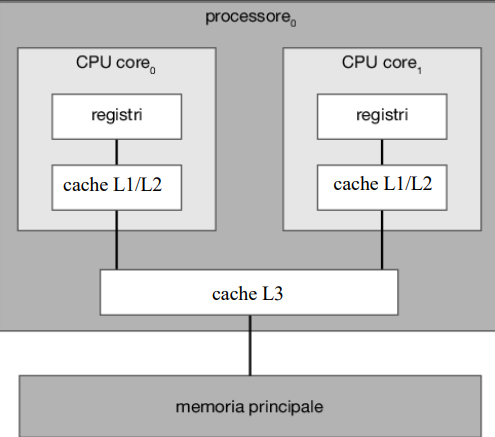
\includegraphics[width=0.5\textwidth]{1/multi-core-architecture.png}
    \caption{Architettura di un processore dual-core}
    \label{fig:multi-core}
\end{figure}

\subsection{Gestione delle Interruzioni}
Il SO è un sistema ``event-driven'', ossia viene attivato quando si verificano eventi come \textit{interrupt} (hardware) o \textit{eccezioni} (software). Ogni interruzione attiva una porzione specifica di codice del SO. La figura \ref{fig:interrupt-handler} rappresenta un esempio di gestione delle interruzioni.


\subsection{Memoria e Cache}
La gerarchia delle memorie include registri, cache, RAM e memoria secondaria. I dati più frequentemente utilizzati vengono spostati in memorie più veloci, come la cache. In figura \ref{fig:memory-hierarchy} si può osservare la gerarchia delle memorie.

\begin{figure}[h!]
    \centering
    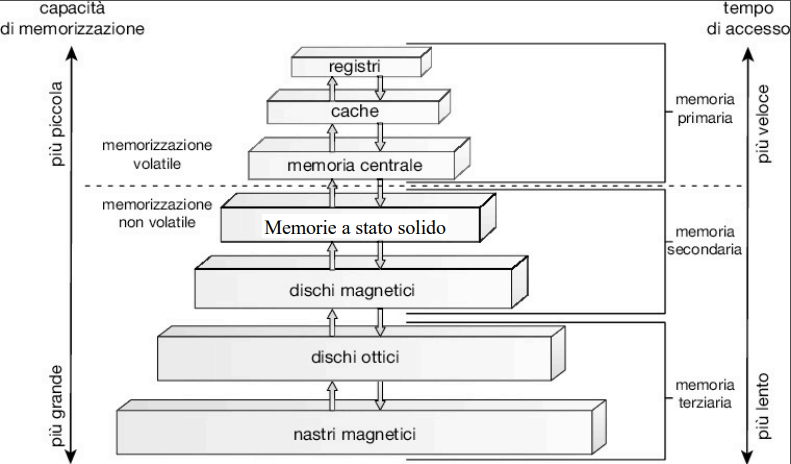
\includegraphics[width=0.5\textwidth]{1/memory-hierarchy.png}
    \caption{Gerarchia delle memorie}
    \label{fig:memory-hierarchy}
\end{figure}

\section{Multitasking e Time-sharing}
Il SO gestisce più programmi contemporaneamente, assegnando la CPU a ciascuno quando disponibile. Il time-sharing permette di distribuire il tempo della CPU tra più utenti, dando l'impressione di simultaneità.

\section{Protezione della Memoria}
Il SO protegge la memoria primaria da accessi non autorizzati attraverso il meccanismo di registri base e limite, come mostrato in figura \ref{fig:memory-protection}.


\afterpage{}

% %---------------------------------------

\definecolor{chaptergrey}{rgb}{0,0.7,0}

\chapter{Strutture dei Sistemi Operativi}
Un sistema operativo mette a disposizione degli utenti (e dei loro programmi) molti servizi 
\begin{figure}[h]
    \centering
    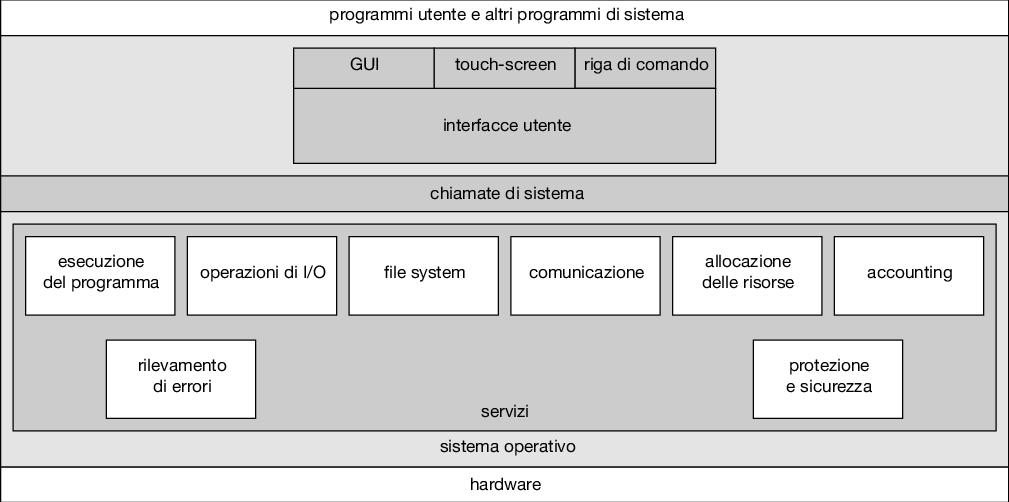
\includegraphics[width=0.5\linewidth]{images/Strutture-di-SO.png}
\end{figure}

Alcuni di questi servizi sono completamente invisibili agli utenti, altri sono parzialmente visibili, e altri sono direttamente usati dagli utenti.
Ma il \textit{grado di visibilità} dipende anche dal tipo di utente (Root, user, group)

\ex{Esempi di visibilità}{
\begin{itemize}
    \item Interfaccia col sistema operativo (terminale) (visibili)
    \item Chiamate di sistema (quasi sempre visibili)
    \item Gestione di processi (praticamente invisibili
\end{itemize}
}

\section{Interfaccia del Sistema Operativo}
L'interfaccia è lo strumento con il quale gli utenti interagiscono con il So, e ne sfruttano i servizi offerti.\\
Può essere un \textbf{interprete di comandi}, o un'\textbf{interfaccia grafica} con finestre e menù, ma di solito è possibile usare una combinazione di entrambi

\subsection{Interprete dei comandi}
Normalmente non fa parte del \textbf{kernel} SO; ma è un programma (o collezione di essi) fornito insieme al SO.\\
Un esempio d'interprete è la \textbf{shell} dell'MS-Dos oppure la \textbf{shell} Unix.\\
Una shell rimane semplicemente in attesa di ciò che l'utente scrive da linea di comando, ed ovviamente, esegue il comando stesso. Spesso, i comandi che possonoe ssere usati dagli utenti del SO sono dei semplici \textbf{eseguibili}. L'interprete si occupa di trovare sull'hard disk e lanciare il codice dell'eseguibile passando eventuali argomenti specificati.
\ex{Comando shell unix}{
\begin{enumerate}
    \item L'utente scrive \textit{rm myfile}
    \item l'interprete cerca un file eseguibile di nome "rm" e lo lancia, passandogli come parameteo "myfile"
\end{enumerate}
}
\nt{
Un comando utile può essere \textit{ps} che ti permette di vedere i processi attaccati alla tua shell
}

\section{Interfaccia grafica}
I moderni SO offrono anche una interfaccia grafica (GUI) per gli utenti, spesso più facile da imparare ed usare.\\
\textbf{Unix} offre varie interfaccie grafiche, sia proprietarie che open-source, come \textbf{KDE} e \textbf{GNOME}, e ogni utente del SO può scegliersi la sua

\section{Programmi/servizi di Sistema}
Non fanno parte del kernel del SO, ma vengono forniti insieme al SO, e rendono più facile, comodo e conveniente l’uso del Sistema.\\
Gli interpreti dei comandi e le interfacce grafiche sono gli esempi più evidenti di programmi di sistema. \\
Oltre a questi: editor, compilatori, browser, task manager etc etc.

\section{Chiamate di sistema (Syscall)}
Da ora in poi, chiameremo un programma in "esecuzione" come \textbf{processo}
Le system call costituiscono la vera e propria interfaccia tra i processi degli utenti e il Sistema Operativo.\\
Ad esempio, in Unix assumono la forma di procedure che possono essere inserite direttamente in programmi scritti con linguaggi ad alto livello (C, C++, …) \\
Sembra di usare una \textbf{subroutine}, ma l’esecuzione della system call trasferisce il controllo al SO, e in particolare alla porzione di codice del SO che implementa la particolare System Call invocata. \\
Ad esempio, in un programma C, per scrivere dentro ad un file:\\
\begin{lstlisting}[language=C]
fd = open("nomefile", O_WRONLY);
i = write(...)
close(fd)
\end{lstlisting}
\textbf{Open, write e close} sono delle syscall

\subsection{Chiamate di sistema: le "API"}
Application Programming Interface
Le API non sono ltro che uno strato intermedio tra le applicazione sviluppate dai programmatori e le syscall, per rendere più \textbf{facile} l'uso e migliorare la \textbf{portabilità} tra versioni.

\ex{Chiamate}{
Ad esempio, la libreria C dell’ambiente Unix è una semplice forma di API. In questa libreria esiste la funzione per aprire un file: \\
\textit{fopen}, \textit{fprintf} e \textit{fclose}
}

\section{Gestione dei processi}
In un dato istante, all’interno di un SO sono attivi più processi (anche se uno solo è in esecuzione, in un dato istante).
Si parla allora di \textbf{Processi Concorrent}, perchè si contendono l'uso delle risorse hardware della macchina. \\
\begin{enumerate}
    \item La CPU
    \item Lo spazio in memoria primaria e secondaria
    \item I dispositivi di input e output
\end{enumerate}
Il SO ha la responsabilità di fare in modo che ogni processo abbia la sua parte di risorse, senza danneggiare e venire danneggiato dal altri processi.\\

Il SO quindi deve gestire tutti gli aspetti riguardo la vita dei processi.\\
\begin{itemize}
    \item Creazione e cancellazione dei processi
    \item Sospensione e riavvio dei processi
    \item Sincronizzazione tra i processi
    \item Comunicazione tra processi
\end{itemize}
Per eseguire un programma deve essere caricato in memoria principale.\\
In un sistema time-sharing, più processi possono essere contemporaneamnte attivi: il loro codie e i loro dati sono caricati in qualche area della RAM. Quindi il SO deve:
\begin{itemize}
    \item Tenere traccia di quali parti della RAM sono utilizzati e da quale processo
    \item Distruibire la RAM tra i processi
    \item Gestire la RAM in base alla necessità e ai cambiamenti
\end{itemize}

\section{Gestione dei file e del filesystem}
Quasi ogni informazione presente in un sistema è contenuta in un file: una raccolta di informazioni denotata da un nome (e di solito da altre proprietà).\\

I file sono organizzati in una struttura \textbf{gerarchica} detta File System, mediante le cartelle (o directory, o folder)
Il SO e’ responsabile della:
– Creazione e cancellazione\\
- Fornitura di strumenti per gestire i file e dir\\
- Memorizzazione efficiente del file system in memoria secondaria.\\

I file sono memorizzati permanentemente in memoria secondaria, di solito su un hard disk.\\
Il SO deve:\\
  – decidere dove e come memorizzare i file su disco, ed essere in grado di ritrovarli velocemente.\\
  – Trovare spazio libero velocemente quando un file è creato o aumenta di dimensione, e recuperare spazio alla rimozione di un file.\\
  – Gestire efficientemente accessi concorrenti ai file dai vari processi attivi.\\

\section{Macchine Virutali}
Un moderno SO trasforma una macchina reale in una sorta di macchina virtuale (MV).


\afterpage{}

\chapter{Gestione dei processi}

\section{Processi}
Il processo è l'unità di lavoro del sistema operativo, perché ciò che fa un qualsiasi SO è innanzi tutto amministrare la vita dei processi che girano sul computer gestito da quel SO.
Il sistema operativo è responsabile della creazione e cancellazione dei processi degli utenti, gestisce lo scheduling dei processi, fornisce dei meccanismi di sincronizzazione e comunicazione fra i processi.\\

\subsection{Concetto di processo}
\begin{itemize}
    \item Un \textbf{processo} è più di un semplice programma in esecuzione, infatti, ha una struttura in memoria primaria, suddivisa in più parti assegnategli dal sistema operativo (vedi fig. 3.1).
    \item Le principali componenti della struttura di un processo sono:
    \begin{itemize}
        \item \textbf{Codice} da eseguire (il "testo")
        \item \textbf{Dati}
        \item \textbf{Stack} (per le chiamate alle procedure/metodi e il passaggio dei parametri)
        \item \textbf{Heap} (memoria dinamica)
    \end{itemize}
    \item La somma di queste componenti forma l'immagine del processo:
    \[
    \text{codice} + \text{dati} + \text{stack} + \text{heap} = \text{immagine del processo}
    \]
\end{itemize}

\begin{figure}[h]
    \centering
    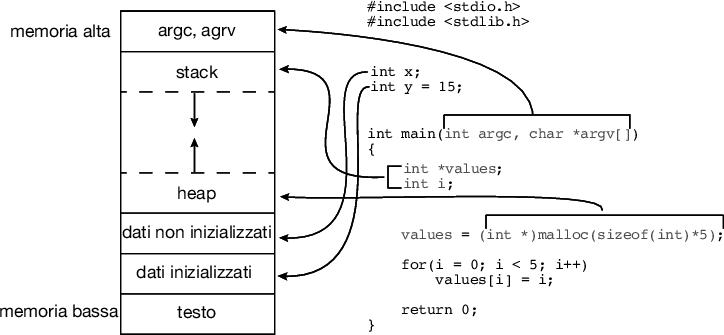
\includegraphics[width=0.5\linewidth]{images/Concetto-di-processo.png}
    \caption{Concetto di processo}
    \label{fig:prco1}
\end{figure}


     È anche corretto osservare che attraverso un programma si possono definire più processi, infatti:
    \begin{itemize}
        \item Lo stesso programma può contenere codice per generare più processi
        \item Più processi possono condividere lo stesso codice
    \end{itemize}
Tuttavia, la distinzione fondamentale tra processo e programma è che un processo \textbf{è un'entità attiva}, mentre un programma è \textbf{un'entità statica}.\\
\qs{}{Lo stesso programma lanciato due volte può dare origine a due processi diversi (perché?)}
Attenzione: processo, task, job sono \textbf{sinonimi}.\\

Un programma si \textbf{trasforma} in un processo quando viene lanciato, con il doppio click o da riga di comando.\\
Un processo può anche \textbf{nascere} a partire da un altro processo, quando quest’ultimo esegue una opportuna system call (fork, spawn, etc)\\

\dfn{Processo}{
In realtà, non sono due meccanismi distinti: un processo nasce sempre a partire da un altro processo, e sempre sotto il controllo e con l’intervento del SO (con un’unica eccezione, all’accensione del sistema).
}
\subsection{Stato del processo}
Da quanto nasce a quando termina, un processo passa la sua esistenza muovendosi tra un insieme di stati, e in ogni stante ogni processo si trova in un ben determinato stato. \\
Lo stato di un processo evolve a causa del codice eseguito e dell’azione del SO sui processi presenti nel sistema in un dato istante, secondo quanto illustrato dal diagramma di transizione degli stati di un processo.\\

\begin{figure}[h]
    \centering
    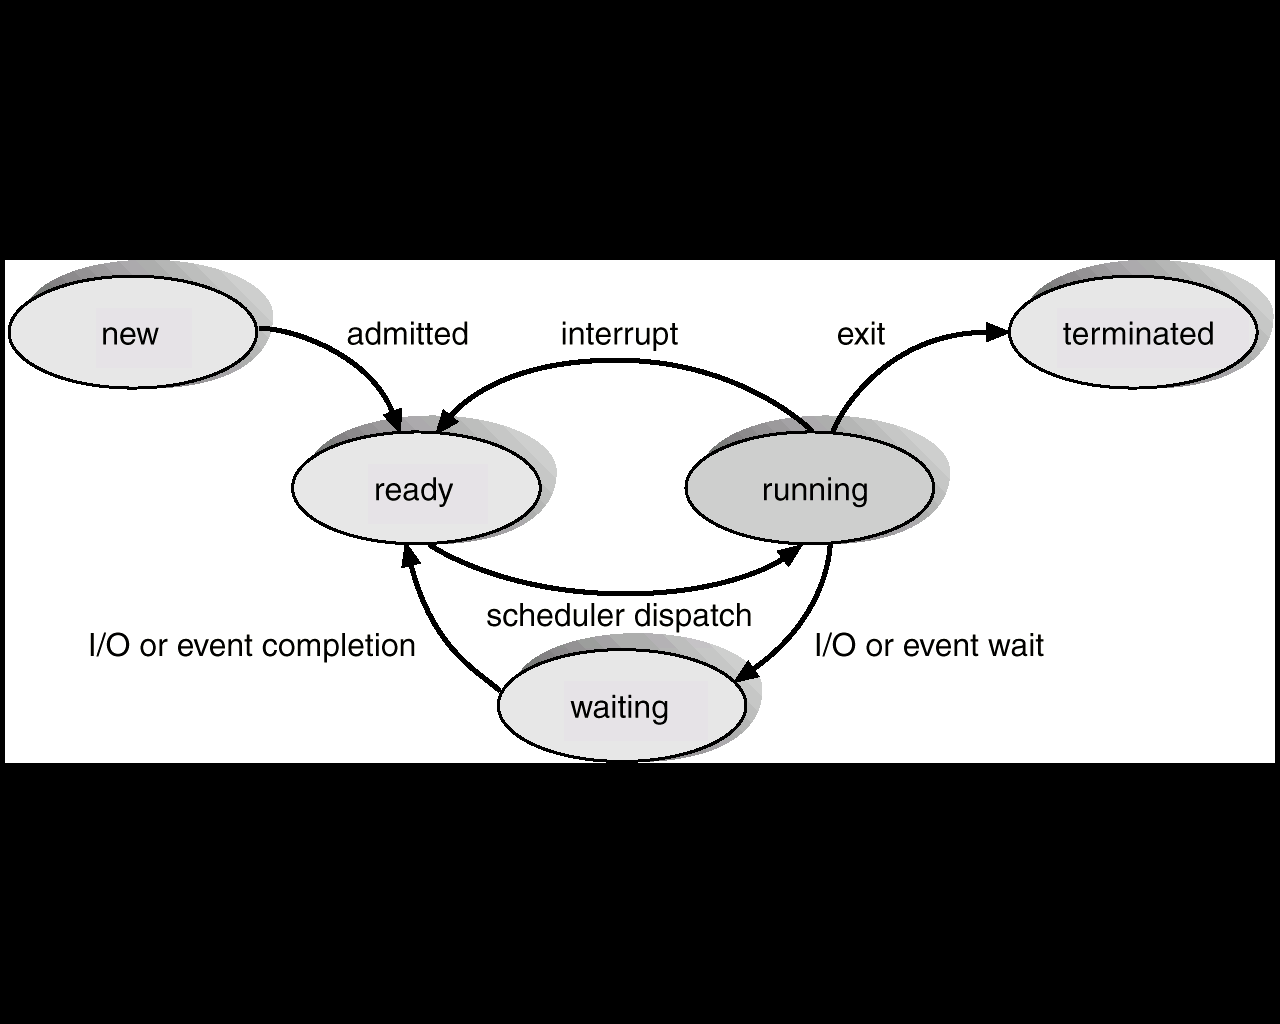
\includegraphics[width=0.5\linewidth]{images/StatoProcesso.png}
\end{figure}

\subsubsection{Gli stati}
Gli stati in cui può trovarsi un processo sono:
\dfn{Stati del processo}{\begin{itemize}
    \item \textbf{New}: Il processo è appena stato creato
    \item \textbf{Ready (to Run)}: Il processo è pronto per entrare in esecuzione
    \item \textbf{Running}: La CPU sta eseguendo il codice del processo
    \item \textbf{Waiting}: Il provesso ha lasciato la CPU e attende il completamento di un evento
    \item \textbf{Terminated}: Il processo è terminato, il SO sta recuperando le strutture dati e le aree di memoria liberate
\end{itemize}
}

Il diagramma di transizione degli stati di un processo sintetizza una serie di possibili varianti del modo in cui un sistema operativo (SO) può amministrare la vita dei processi di un computer.

\begin{itemize}
    \item Infatti, nel caso reale lo sviluppatore del SO dovrà decidere quali scelte implementative fare quando (ad esempio):
    \begin{itemize}
        \item Mentre il processo \(P_x\) è \textit{running}, un processo entra nello stato \textit{Ready to Run}
        \item Mentre il processo \(P_x\) è \textit{running}, un processo più importante di \(P_x\) entra nello stato \textit{Ready to Run}
        \item Mentre il processo \(P_x\) è nello stato \textit{Ready to Run}, un processo più importante di \(P_x\) entra nello stato \textit{Ready to Run}
    \end{itemize}
\end{itemize}

\qs{}{
Che significato ha eliminare l’arco “interrupt”?
}

Di avere un sistema non time-sharing

\subsection{Processo Control Block (PCB)}
Per ogni processo, il sistema operativo (SO) mantiene una struttura dati chiamata \textit{Process Control Block} (PCB), che contiene le informazioni necessarie per amministrare la vita di quel processo, tra cui:

\begin{itemize}
    \item Il numero del processo (o \textit{Process ID})(PID)
    \item Lo stato del processo (\textit{ready}, \textit{waiting},...)
    \item Il contenuto dei registri della CPU salvati nel momento in cui il processo è stato sospeso (valori significativi solo quando il processo non è \textit{running})
    \item Gli indirizzi in RAM delle aree dati e codice del processo
    \item I file e gli altri dispositivi di I/O correntemente in uso dal processo
    \item Le informazioni per lo \textit{scheduling} della CPU (ad esempio, quanta CPU ha usato fino a quel momento il processo)
\end{itemize}

\begin{figure}
    \centering
    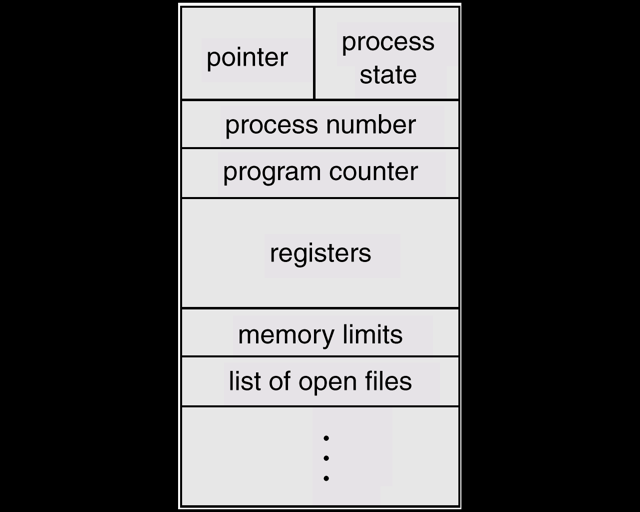
\includegraphics[width=0.5\linewidth]{images/Process-Control-Block.png}
\end{figure}

\section{Scheduling dei processi}
Conosciamo già i seguenti due concetti:

\begin{itemize}
    \item \textbf{Multiprogrammazione}: avere sempre un processo \textit{running} \(\Rightarrow\) massima utilizzazione della CPU.
    \item \textbf{Time Sharing}: distribuire l'uso della CPU fra i processi a intervalli prefissati. Così più utenti possono usare "allo stesso tempo" la macchina, e i loro processi procedono in "parallelo" (notate sempre le virgolette).
\end{itemize}

\dfn{Scheduling}{
Per implementare questi due concetti, il sistema operativo deve decidere periodicamente quale sarà il prossimo processo a cui assegnare la CPU. Questa operazione è detta \textit{Scheduling}.
}

In un sistema time sharing single-core, attraverso lo scheduling, ogni processo “crede” di avere a disposizione una macchina “tutta per se”...
Ci pensa il SO a farglielo credere, \textbf{commutando} la CPU fra i processi (ma succede la stessa cosa in un sistema ad n-core se ci sono più di n processi attivi contemporaneamente)
\begin{figure}[h]
    \centering
    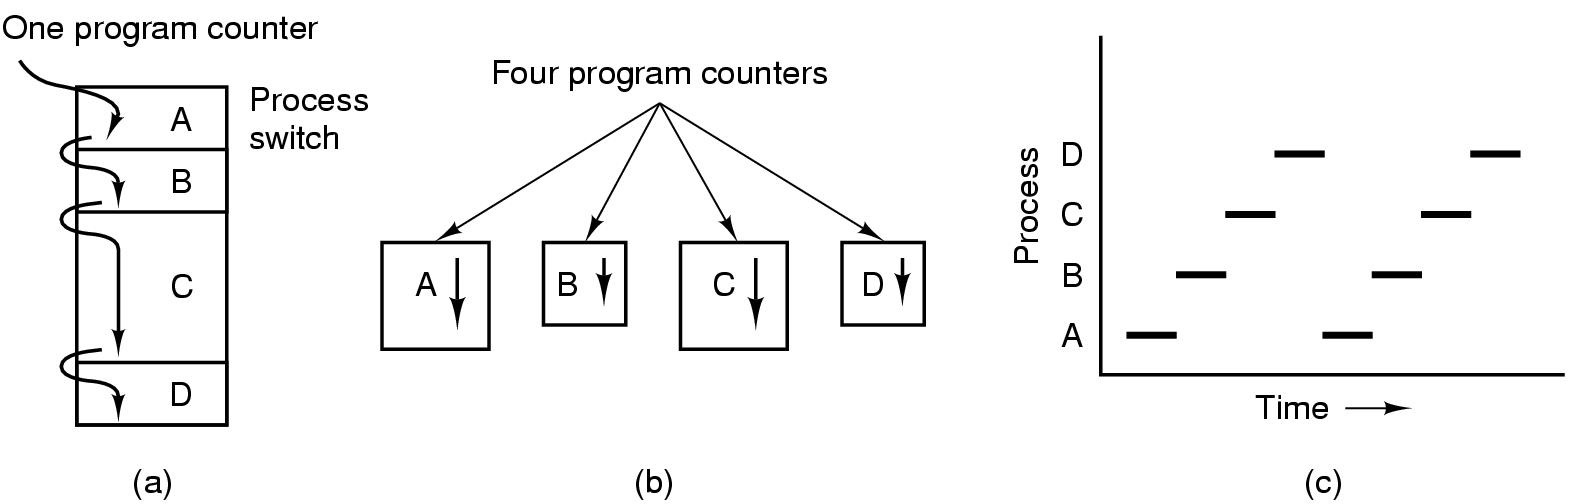
\includegraphics[width=0.5\linewidth]{images/SchedulingProcessi.png}
    \caption{a) Ciò che succede in realtà\\b) ciò che vede ogni singolo processo\\c) Il risultato finale}
\end{figure}

\subsection{Il cambio di contesto (context switch)}
Per commutare la CPU tra due processi, il sistema operativo deve:

\begin{enumerate}
    \item Riprendere il controllo della CPU (ad esempio attraverso il meccanismo del \textit{Timer} visto nel capitolo 1).
    \item Con l'aiuto dell'hardware della CPU, salvare lo stato corrente della computazione del processo che lascia la CPU, ossia copiare il valore del \textit{Program Counter} (PC) e degli altri registri nel suo \textit{Process Control Block} (PCB).
    \item Scrivere nel PC e nei registri della CPU i valori relativi contenuti nel PCB del processo utente scelto per entrare in esecuzione.
\end{enumerate}
Questa operazione prende il nome di: \textbf{cambio di contesto}, o \textit{context switch}.

Notate che, tecnicamente, anche il punto 1 è già di per sé un \textit{context switch}.

\begin{itemize}
    \item Il \textit{context switch} richiede tempo, perché il contesto di un processo è composto da molte informazioni (alcune le vedremo quando parleremo della gestione della memoria).
    \item Durante questa frazione di tempo, la CPU non è utilizzata da alcun processo utente.
    \item In generale, il \textit{context switch} può costare da qualche centinaio di nanosecondi a qualche microsecondo.
    \item Questo tempo “sprecato” rappresenta un \textit{overhead} (sovraccarico) per il sistema e influisce sulle sue prestazioni.
\end{itemize}

\begin{figure}[h]
    \centering
    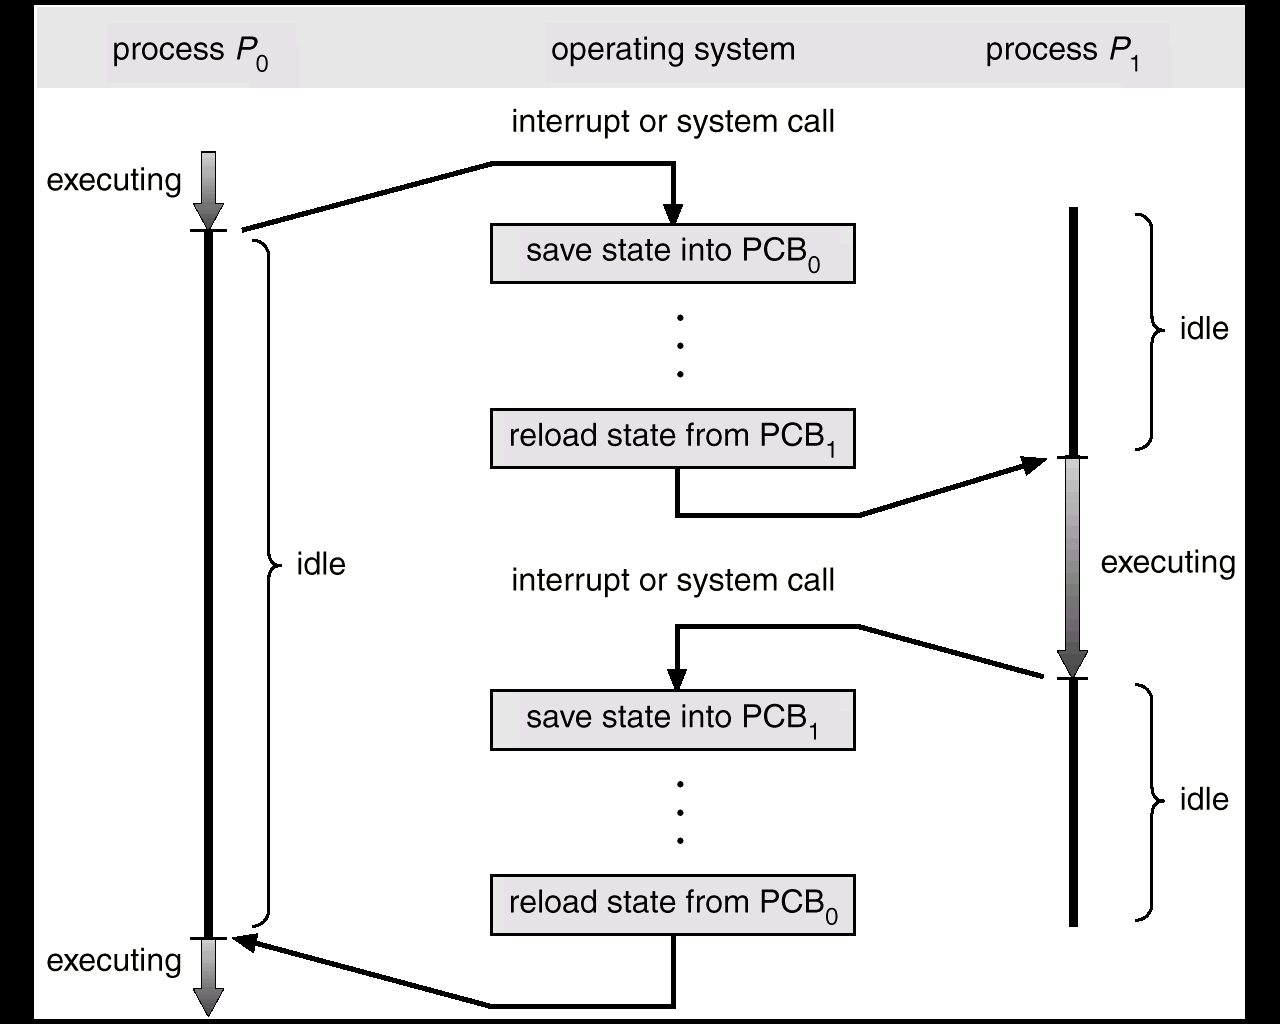
\includegraphics[width=0.5\linewidth]{images/Phases_of_scheduling.png}
    \caption{Fasi dello scheduling tra un processo e un altro}
\end{figure}

\subsection{Code di scheduling}
Per \textbf{amministrare} la vita di ciascun processo, il SO gestisce varie \textbf{code} di processi. Ogni processo “si trova” in una di queste code, a seconda di cosa sta facendo.
Una coda di processi non è altro che una lista di PCB, mantenuta in una delle aree di memoria primaria che il SO riserva a se stesso.\\
La coda dei processi più importante è la coda \textbf{ready}, o \textbf{ready queue (RQ)}: l'insieme dei processi \textbf{ready to run}.
\begin{figure}[h]
    \centering
    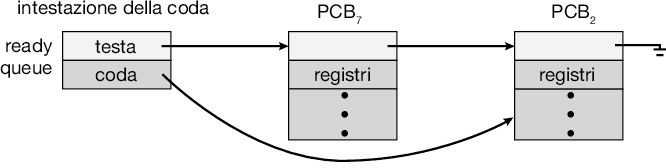
\includegraphics[width=0.5\linewidth]{images/ready_queue.png}
    \label{fig:ready_queue}
\end{figure}
Quando un processo rilascia la CPU, ma non termina e non torna nella \textit{ready queue}, vuol dire che si è messo in \textbf{attesa} di “qualcosa”, e il SO lo “parcheggia” in una tra le possibili code, che possiamo dividere in due grandi categorie:
\begin{itemize}
    \item \textbf{Device queues}: code dei processi in attesa per l’uso di un dispositivo di I/O. Una coda per ciascun dispositivo.
    \ex{Esempi}{
        \item Una coda d'attesa per il primo hard disk
        \item Una coda per l'ssd
        \item Una coda per la stampante, etc..
    }
    \item \textbf{Code di waiting}: code di processi in attesa che si verifichi un certo evento. Una coda per ciascun evento (ci torneremo nella sezione 6.6).
\end{itemize}
Dunque, durante la loro vita, i processi si spostano (meglio: il SO sposta i corrispondenti PCB) tra le varie code.\\
Quindi lo stato \textbf{waiting} nel diagramma di transizione degli stati di un processo \textbf{corrisponde a più code di attesa}

Possiamo riformulare il diagramma di transizione degli stati di un processo come un \textbf{diagramma di accodamento} in cui i processi si muovono fra le varie code 

\begin{figure}[h]
    \centering
    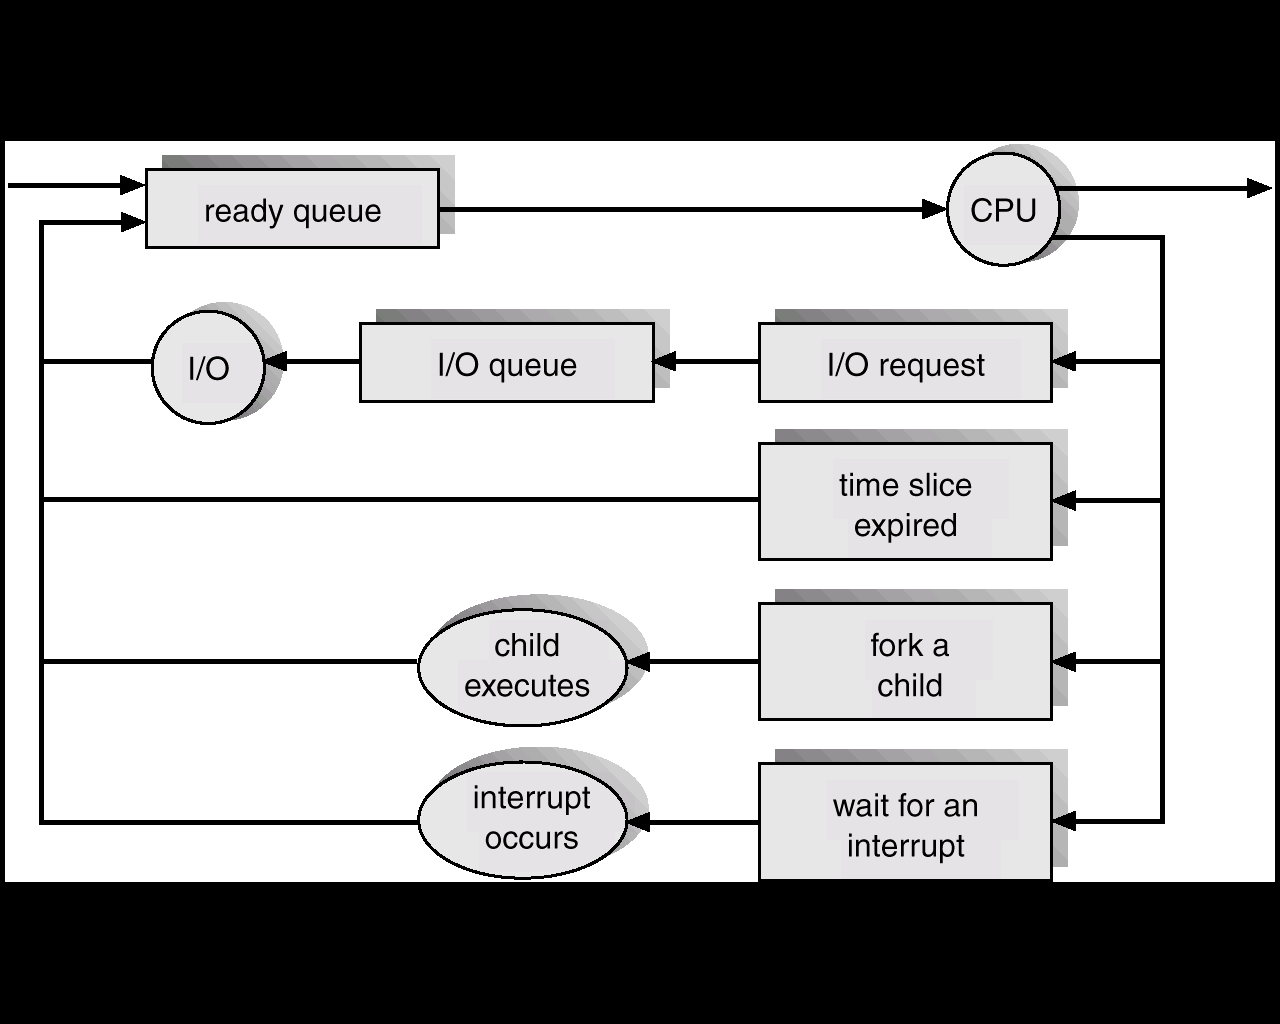
\includegraphics[width=0.5\linewidth]{images/Scheduling_queue_updated.png}
    \caption{SX: new, DX: Terminated}
\end{figure}

\subsection{CPU Scheduler}

Un componente del Sistema Operativo detto \textit{CPU Scheduler} sceglie uno dei processi nella coda \textit{ready} e lo manda in esecuzione.
\begin{itemize}
    \item Il \textit{CPU scheduler} si attiva ogni 50/100 millisecondi, ed è responsabile della realizzazione del \textit{time sharing}.
    \item Per limitare l'\textit{overhead}, deve essere molto veloce.
    \item Il \textit{CPU scheduler} è anche chiamato \textit{Short Term Scheduler}.
\end{itemize}


\section{Operazione sui processi}
La creazione di un processo è di gran lunga l’operazione più importante all’interno di qualsiasi sistema operativo.\\
Ogni SO possiede almeno una \textit{System Call} per la creazione di processi, e ogni processo è creato a partire da un altro processo usando la system call relativa (eccetto il processo che nasce all’accensione del sistema).\\
Il processo "creatore" è detto \textit{processo padre} (o \textit{parent}).\\
Il processo creato è detto \textit{processo figlio} (o \textit{child}).
\clm{}{}{
Poiché ogni processo può a sua volta creare altri processi, nel sistema si forma un “albero di processi”.}
\begin{figure}[h]
    \centering
    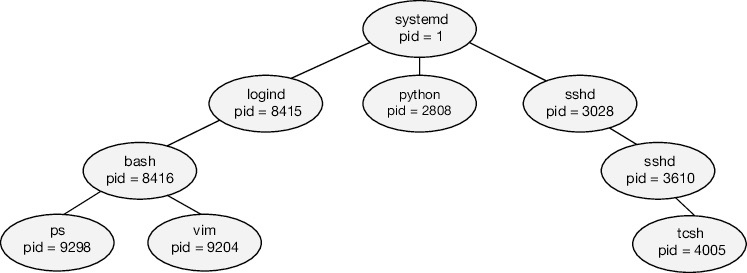
\includegraphics[width=0.5\linewidth]{images/Process_creation.png}
    \label{fig:creation_process}
\end{figure}

\subsection{Creazione di un processo}
Quando nasce un nuovo processo, il SO:
\begin{itemize}
    \item gli assegna un identificatore del processo unico, un numero intero detto \textbf{pid} (process-id). È il modo con cui il SO conosce e si riferisce a quel processo.
    \item recupera dall’hard disk il codice da eseguire e lo carica in RAM (a meno che il codice non sia già in RAM).
    \item alloca un nuovo \textit{PCB} e lo inizializza con le informazioni relative al nuovo processo.
    \item inserisce il \textit{PCB} in coda \textit{ready}.
\end{itemize}

\qs{}{Che cosa fa il processo padre quando ha generato un
processo figlio?}
\begin{itemize}
    \item Prosegue la sua esecuzione in modo concorrente all'esecuzione del processo figio, oppure:
    \item  Si ferma, in attesa del completamento dell'esecuzione del processo figlio
\end{itemize}
\qs{}{Quale codice esegue il processo figlio?}
\begin{itemize}
    \item al processo figlio viene data una copia del codice e dei dati in uso al processo padre, oppure:
    \item al processo figlio viene dato un nuovo programma, con eventualmente nuovi dati.
\end{itemize}

\subsection{Creazione di un processo in Unix}
\begin{lstlisting}[language=C]
int main() {
    /* fig. 3.8 modificata */
    pid_t pid, childpid;
    
    pid = fork(); /* genera un nuovo processo */
    printf("questa la stampano padre e figlio");
    
    if (pid == 0) { 
        /* processo figlio */
        printf("processo figlio");
        execlp("/bin/ls", "ls", NULL);
    } else {
        /* processo padre */
        printf("sono il padre, aspetto il figlio");
        childpid = wait(NULL);
        printf("il processo figlio e' terminato");
        exit(0);
    }
}
\end{lstlisting}

\subsection{Passi dell'SO all'invocazione delle fork}
\begin{enumerate}
    \item Alloca un nuovo \textit{PCB} per il processo figlio e gli assegna un nuovo \textit{PID}; cerca un’area libera in RAM e vi copia le strutture dati e il codice del processo \textit{parent} (si veda più avanti): queste copie verranno usate dal processo figlio.
    \item Inizializza il \textit{PC} del figlio con l’indirizzo della prima istruzione successiva alla \textit{fork}.
    \item \textbf{Nella cella di memoria associata alla variabile che riceve il risultato della \textit{fork} del processo figlio scrive 0.}
    \item \textbf{Nella cella di memoria associata alla variabile che riceve il risultato della \textit{fork} del processo \textit{parent} scrive il \textit{PID} del figlio.}
    \item Mette i processi \textit{parent} e figlio in coda \textit{ready}.
\end{enumerate}

\clm{}{}{
$pid == 0$ Lo ha solo il processo figlio. \\
pid = id-child lo ha solo il processo padre. \\
Così sono in grado di distinguere se sto operando con il figlio o con il padre.
}

\subsubsection{Significato delle altre sys}
\textbf{Execlp}: Riceve in input un puntatore ad un file contenente codice eseguibile. Il processo che la invoca prosegue eseguendo il codice specificato, senza più ritornare alla porzione di codice che viene dopo la execlp.\\
\textbf{Wait}: Invocata da un processo parent, lo sospende fino alla terminazione del processo figlio. La wait restituisce il PID del figlio appena terminato.
\textbf{Exit:} provoca la terminazione istantanea del processo che la invoca.\\

\qs{}{Come cambia lo schema se il processo parent non esegue la wait?}
\begin{figure}[h]
    \centering
    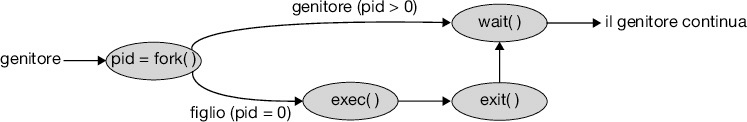
\includegraphics[width=0.5\linewidth]{images/child&parentLoveandFriend.png}
\end{figure}

\subsection{Altro esempio}
\begin{lstlisting}[language=C]
int main() {
    /* un altro esempio */
    int a, b, c = 57;
    a = fork(); // genera un nuovo processo
    printf("questa la stampano padre e figlio");
    
    if (a == 0) {
        /* processo figlio */
        c = 64; // ***
        printf("c = %d", c);
    } else {
        /* processo padre */
        printf("c = %d", c);
        b = wait(NULL);
        printf("b = %d", b);
    }
}
\end{lstlisting}
\subsection{Osservazioni}
\begin{itemize}
    \item Il codice viene condiviso tra padre e figlio, evitando duplicazione e spreco di memoria.
    \item Lo spazio dati viene duplicato: 
    \begin{itemize}
        \item Le modifiche di variabili non sono condivise tra padre e figlio.
        \item Le nuove variabili dichiarate dopo la \texttt{fork} non sono visibili all'altro processo.
    \end{itemize}
    \item Un padre può chiamare \texttt{fork} più volte, e usare il PID dei figli per tracciarli.
    \item \texttt{fork} restituisce 0 al figlio per distinguerlo dal padre.
    \item Se \texttt{fork} restituisse un valore maggiore di 0 al figlio, non si potrebbe distinguere facilmente tra padre e figlio, complicando la gestione delle operazioni diversificate (come illustrato in fig. 3.8).
\end{itemize}

\subsection{Terminazione di un processo}
Un processo termina dopo l'esecuzione dell'ultima istruzione del suo codice. Esiste una system call chiamata \texttt{exit()} per terminare un processo. \\
I dati di output, come il \texttt{pid}, possono essere inviati al processo padre in attesa della terminazione del figlio.
Il sistema operativo \textbf{rimuove} le risorse allocate al processo terminato, recuperando la RAM e chiudendo eventuali file aperti.

\begin{itemize}
    \item Un processo può uccidere esplicitamente un altro processo appartenente allo stesso utente tramite la system call \texttt{kill} (in Unix) o \texttt{TerminateProcess} (in Win32).
    \item In alcuni casi, il sistema operativo può decidere di terminare un processo utente, ad esempio se:
    \begin{itemize}
        \item il processo utilizza troppe risorse.
        \item il suo processo padre è morto (in questo caso può avvenire una terminazione a cascata, che non avviene però in Unix o Windows).
    \end{itemize}
\end{itemize}

\section{Comunicazione tra processi}
\textbf{Processi indipendenti e cooperanti}

I processi attivi in un sistema possono essere classificati come:

\begin{itemize}
    \item \textbf{Indipendenti}: quando non si influenzano esplicitamente durante l'esecuzione.
    \item \textbf{Cooperanti}: quando si influenzano a vicenda per:
    \begin{itemize}
        \item Scambiarsi informazioni.
        \item Collaborare su un'elaborazione suddivisa per efficienza o modularità.
    \end{itemize}
\end{itemize}

I processi cooperanti necessitano di meccanismi di comunicazione e sincronizzazione.

\section{Esempio: il problema Produttore-Consumatore}
\textbf{Problema del produttore-consumatore}

Un classico problema di processi cooperanti è il \textit{problema del produttore-consumatore}:

\begin{itemize}
    \item Un \textbf{processo produttore} produce informazioni che vengono consumate da un \textbf{processo consumatore}.
    \item Le informazioni sono collocate in un buffer di dimensione limitata.
    \item Un esempio pratico è un \textbf{processo compilatore} (produttore) che genera codice assembler.
    \item Il \textbf{processo assemblatore} (consumatore) traduce il codice assembler in linguaggio macchina.
    \item L'assemblatore potrebbe poi diventare un produttore per un modulo che carica in RAM il codice.
\end{itemize}

\begin{lstlisting}[language=C]
#define SIZE 10

typedef struct {
    // Definizione della struttura dell'item
    ...
} item;

// Buffer condiviso
item buffer[SIZE]; (shared array)

// Variabili condivise
int in = 0, out = 0; 
\end{lstlisting}

\textbf{Buffer circolare} di \texttt{SIZE} elementi con due puntatori \texttt{in} e \texttt{out}:
\begin{itemize}
    \item \texttt{in}: indica la prossima posizione libera nel buffer.
    \item \texttt{out}: indica la prossima posizione piena da consumare.
    \item \textbf{Condizione di buffer vuoto}: \texttt{in == out}.
    \item \textbf{Condizione di buffer pieno}: \texttt{(in + 1) \% SIZE == out}.
\end{itemize}

\textit{Nota}: la soluzione utilizza solo \texttt{SIZE-1} elementi per evitare conflitti tra la condizione di buffer pieno e vuoto.

\subsection{Inter-Processo Comunication (IPC)}

\qs{}{
Come fanno due processi a scambiarsi le informazioni necessarie alla cooperazione?
}
\begin{itemize}
    \item Il Sistema Operativo (SO) fornisce dei meccanismi di \textbf{Inter-Process Communication (IPC)}.
    \item Sono disponibili opportune \textbf{system call} che permettono a due (o più) processi di:
    \begin{itemize}
        \item \textbf{scambiarsi messaggi} oppure
        \item \textbf{usare la stessa area di memoria condivisa}, in cui possono scrivere e leggere.
    \end{itemize}
\end{itemize}
\begin{figure}[h]
    \centering
    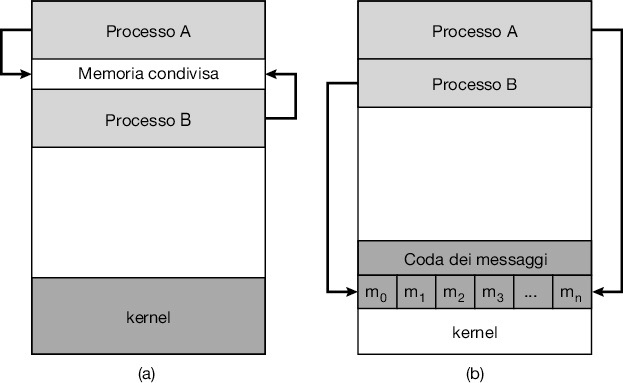
\includegraphics[width=0.5\linewidth]{images/IPC_graphic.png}
    \caption{a) Memoria condivisa\\b) Scambio di messaggi}
\end{figure}

In entrambi i casi, il SO mette a disposizione delle opportune \textbf{system call}. Ad esempio, per lo scambio di messaggi, saranno disponibili delle system call del tipo:

\begin{itemize}
    \item \texttt{line = msgget();}
    \item \texttt{send(message, line, process-id);}
    \item \texttt{receive(message, line, process-id);}
\end{itemize}

\textbf{(Nota:)} I parametri sono solo indicativi, ogni specifica implementazione avrà il proprio insieme di argomenti.

\bigskip
Saranno necessarie alcune \textbf{scelte implementative}. 

Nel caso dei \textbf{messaggi} (si parla spesso di \emph{code di messaggi}):
\begin{itemize}
    \item Una coda può essere usata da più di due processi?
    \item Quanti messaggi può ospitare al massimo una coda?
    \item Cosa deve fare un processo ricevente se non ci sono messaggi, o un processo trasmittente se la linea è piena?
    \item Si possono trasmettere messaggi di lunghezza variabile?
\end{itemize}

Nel caso della \textbf{memoria condivisa}:
\begin{itemize}
    \item Può avere dimensione variabile?
    \item Quali processi hanno diritto di usarla?
    \item Cosa succede se la memoria condivisa viene rimossa?
\end{itemize}



\afterpage{}

\chapter{Threads}
\nt{
    Questo capitolo va studiato solo dopo il capitolo 9 sulla memoria centrale. Ai fini del programma del corso e dell’esame, si fa riferimento a queste slide, il cui contenuto è molto semplificato rispetto al capitolo 4 del libro di testo.
}

Consideriamo due processi che devono lavorare sugli stessi dati. Come possono farlo, se ogni processo ha la propria area dati (ossia, gli spazi di indirizzamento dei due processi sono separati)?

\begin{itemize}
    \item I due processi possono richiedere al sistema operativo un’area di memoria condivisa, oppure scambiarsi i dati usando messaggi.
    \item I dati possono essere mantenuti in un file, al quale i due processi accedono a turno.
\end{itemize}

Sarebbe comodo poter avere processi in grado di lavorare sugli stessi dati senza usare meccanismi espliciti di condivisione/comunicazione, e senza l’utilizzo di file, che risiedono su supporti relativamente lenti. Ad esempio, in un editor di testo:
\begin{itemize}
    \item Un processo gestisce l’input e i comandi di formattazione dell’utente;
    \item Un altro processo esegue il controllo automatico degli errori.
\end{itemize}

In questo caso, i due processi dovrebbero poter lavorare sullo stesso testo, la cui copia corrente è mantenuta in memoria principale. Tuttavia, poiché ogni processo ha un diverso spazio di indirizzamento, come possono lavorare sulla stessa copia dei dati?

Inoltre, durante il \textit{context switch} tra processi, occorre disattivare le aree dati e di codice del processo uscente e attivare quelle del processo entrante. 

\begin{itemize}
    \item Le \textbf{cache fisiche della CPU} contengono ancora i dati del processo uscente, quindi il processo entrante inizialmente genera molti \textit{miss cache}.
    \item Se due (o più) processi potessero condividere dati e codice, il context switch tra di loro sarebbe molto meno oneroso.
\end{itemize}

Da queste considerazioni nasce il concetto di \textbf{thread}: un gruppo di \textit{peer thread} è un insieme di “processi” che condividono lo spazio di indirizzamento (codice e dati).

\dfn{Terminologia}{
    Un processo $P$ (per come è stato studiato finora) è caratterizzato da un unico \textbf{Thread} di computazione: una sequenza di istruzioni eseguite, che ovviamente può cambiare da un’esecuzione all’altra in base, ad esempio, ai dati di input. (Fig. 4.1a).
}

Nessun altro processo ha accesso allo spazio di indirizzamento logico di $P$, quindi nessun processo utente, oltre a $P$, può accedere alle aree dati di $P$. Altri processi possono eseguire lo stesso codice di $P$, ma in uno spazio di indirizzamento logico separato e quindi con dati diversi. (Fig. 4.1a).

\section{Processo Multi-Thread}
Un \textbf{processo Multi-Thread} (o \textbf{Multi-Threaded}) è invece composto da più thread di computazione, detti \textit{peer thread}. Un processo multi-threaded è anche detto \textit{task} (Fig. 4.1).
\begin{figure}[h] \centering 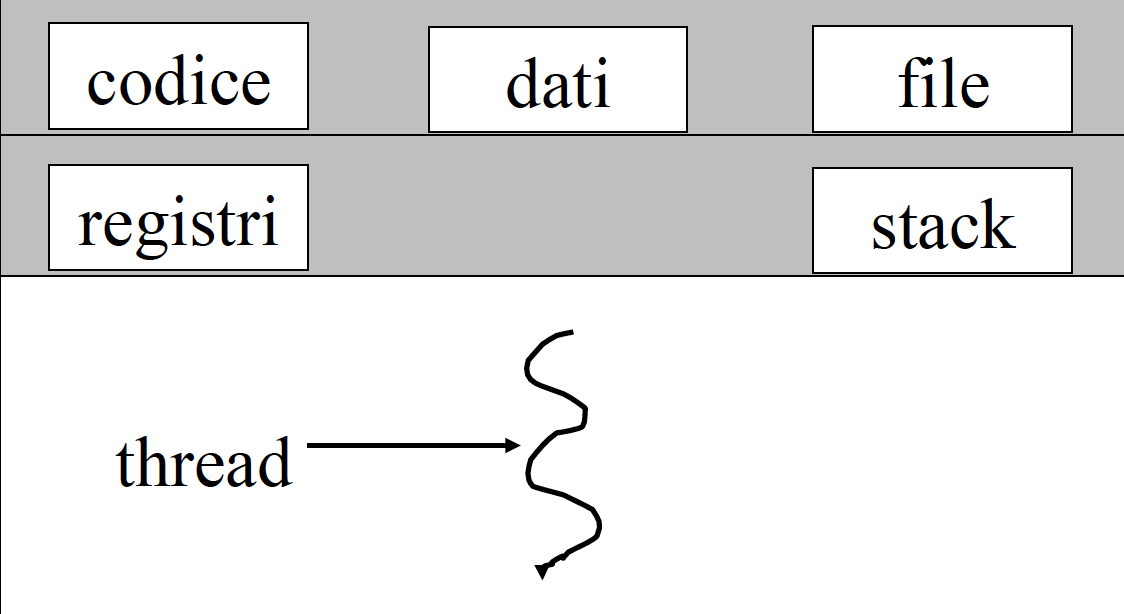
\includegraphics[width=0.50\linewidth]{images/thread_example.png} \caption{thread_example} \label{fig:4.1a} \end{figure}

\begin{figure}[h] \centering 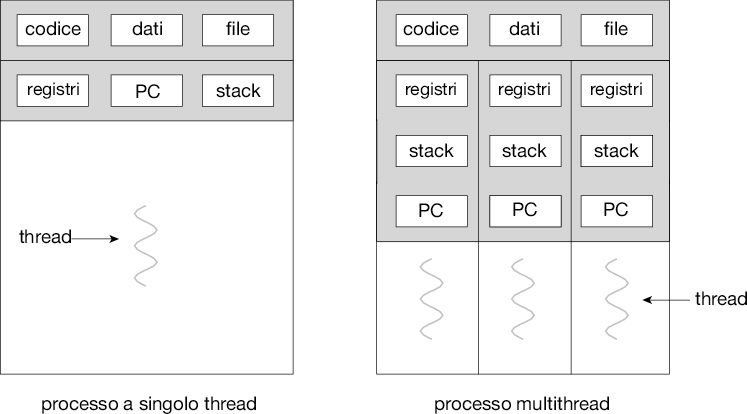
\includegraphics[width=0.50\linewidth]{images/MultiThreadExample.png} \caption{MultiThreadExample.png} \label{fig:4.2} \end{figure}
\dfn{Processo Multi-Thread}{
    Un processo \textbf{Multi-Thread} (o \textbf{Multi-Threaded}) è composto da più thread di computazione, detti \textit{peer thread}. Un processo multi-threaded è anche detto \textit{task} (Fig. 4.1).
}

Ad ogni \textit{peer thread} viene assegnata l’esecuzione di codice, che solitamente è diverso da quello degli altri peer thread. Di conseguenza:

\begin{itemize}
    \item Ogni thread ha uno stato di computazione autonomo, costituito da:
        \begin{itemize}
            \item \textbf{Program Counter} e registri della CPU
            \item uno \textbf{stack} indipendente
        \end{itemize}
    \item Tuttavia, un insieme di \textit{peer thread} condivide il codice in esecuzione e, soprattutto, le \textbf{aree dati}.
\end{itemize}

Il codice deve specificare quale \textit{peer thread} esegue ciascuna parte del codice, similmente a come, in un programma che utilizza la \texttt{fork}, si può definire la porzione di codice eseguita dal processo padre e quella eseguita dal processo figlio.

\clm{}{Context Switch tra Peer Thread}{
    Il \textit{context switch} avviene anche tra ciascun \textit{peer thread} di un processo multi-threaded, per permettere a ciascuno di continuare l’esecuzione del proprio codice assegnato. (Per ora si considera un’architettura \textbf{single core}.)
    
    \begin{itemize}
        \item Il \textit{context switch} tra \textit{peer thread} richiede solo il salvataggio e il ripristino del Program Counter, dei registri della CPU e dello stack, che sono distinti per ogni thread.
        \item Il codice e i dati, cioè lo \textbf{spazio di indirizzamento logico}, rimangono invariati tra \textit{peer thread}, per cui non è necessario cambiare la tabella delle pagine del processo multi-threaded durante il \textit{context switch}.
    \end{itemize}
}

Il \textit{context switch} tra processi è molto più oneroso per il SO rispetto a quello tra peer thread, poiché nel primo caso devono essere cambiate molte più informazioni.

\begin{itemize}
    \item A causa della gestione delle cache, il \textit{context switch} tra processi genera inizialmente più \textit{cache miss} rispetto a quello tra peer thread.
    \item Per questa ragione, i processi normali (quelli studiati finora) sono spesso chiamati \textbf{heavy-weight process} (HWP), mentre i \textit{peer thread} sono definiti \textbf{light-weight process} (LWP).
\end{itemize}

All'interno di un \textit{task}, nuovi peer thread possono essere creati tramite apposite \textit{system call}, e a ciascun thread può essere assegnato codice specifico da eseguire, in modo simile a quanto avviene con \texttt{fork} ed \texttt{exec}. (In \textbf{Linux} un nuovo thread si crea con la system call \texttt{clone}, mentre in \textbf{Windows} con \texttt{CreateThread}.)

\nt{
    Altre \textit{system call} permettono ai peer thread di sincronizzarsi fra loro, analogamente a come i processi possono sincronizzarsi tramite semafori. La sincronizzazione è fondamentale per garantire un accesso ordinato ai dati condivisi tra i thread. Inoltre, molti linguaggi moderni, come Java, offrono primitive apposite per la programmazione multi-threaded.
}

In tutti i sistemi operativi moderni, la gestione dello \textbf{scheduling} dei thread avviene a livello di \textit{kernel}. Il SO mantiene strutture dati per gestire sia i processi normali che tutti i peer thread di un \textit{task} multi-threaded.

\begin{itemize}
    \item Quando un thread si blocca volontariamente o termina il suo quanto di tempo, è il SO a gestire l'assegnazione della CPU, decidendo se assegnarla:
        \begin{itemize}
            \item ad un altro \textit{peer-thread} dello stesso task,
            \item ad uno dei \textit{peer-thread} di un altro task,
            \item oppure ad un processo normale.
        \end{itemize}
\end{itemize}
\nt{
    In Solaris, la creazione di un nuovo \textbf{LWP} (light-weight process) richiede circa 30 volte meno tempo rispetto alla creazione di un \textbf{HWP} (heavy-weight process). Inoltre, il \textit{context switch} tra peer thread è cinque volte più rapido rispetto al \textit{context switch} tra processi.
}

\begin{itemize}
    \item \textbf{Condivisione di dati e risorse}: più thread possono accedere e operare su dati condivisi in modo efficiente, anche se devono essere sincronizzati adeguatamente per evitare condizioni di gara o accessi non sicuri ai dati.
    \item \textbf{Architetture multi-core}: i thread sono particolarmente idonei per essere eseguiti su processori multi-core e, ancor di più, su architetture multithreaded.
\end{itemize}

In un processore \textit{single-core}, tutti i \textit{peer thread} di un task si alternano in esecuzione esattamente come un insieme di processi (Figura 4.3). Come già osservato, il \textit{context switch} tra vari \textit{peer thread} è meno oneroso rispetto al \textit{context switch} tra processi normali. Tuttavia, un \textit{context switch} con un altro processo rimane oneroso e può causare un degrado nelle prestazioni a causa dei miss di cache generati inizialmente dal processo entrante.

\begin{itemize}
    \item \textbf{Architetture multi-core e task multi-threaded}: le architetture multi-core sono particolarmente adatte alla gestione di task multi-threaded. Supponiamo un sistema \textbf{dual-core} in cui sono attivi due task multi-threaded: se si assegna un task a ciascun core, i \textit{context switch} tra thread saranno limitati ai soli \textit{peer thread} del medesimo task, ottimizzando l’efficienza.
    \item \textbf{Bilanciamento del carico}: in pratica, il numero totale di task multi-threaded (e quindi di \textit{peer thread}) è spesso superiore al numero di core disponibili. Il sistema operativo distribuisce quindi i \textit{peer thread} di uno stesso task su core diversi per bilanciare il carico di lavoro in modo ottimale (Figura 4.4 mostra un task con 4 \textit{peer thread} distribuito su due core).
\end{itemize}

\cor{Opportunità di esecuzione parallela nei processori moderni}{
    I processori moderni offrono un'opportunità ulteriore per l'esecuzione dei thread. In un processore multicore, ciascun core è in grado di eseguire fino a 4 o 5 istruzioni in parallelo del programma in esecuzione; questa tecnica è nota come \textbf{multiple issue}.
    
    \begin{itemize}
        \item Per eseguire più istruzioni in parallelo, ogni core deve disporre di più unità funzionali, come le ALU (Arithmetic Logic Units) e le unità di calcolo in virgola mobile. Tale struttura è detta \textit{superscalare}, poiché consente a ciascun core di eseguire in parallelo fino a 4 o 5 istruzioni, migliorando l'efficienza complessiva del sistema.
    \end{itemize}
}


\section{CPU/Core multi-threaded}

I processori moderni offrono un'importante opportunità per l'esecuzione dei thread grazie alla capacità di eseguire in parallelo più istruzioni per ciclo di clock. Questa tecnica, chiamata \textbf{multiple issue}, consente a ciascun core di avviare fino a 4 o 5 istruzioni contemporaneamente. Ciò è possibile grazie alla presenza di più unità funzionali in ogni core, come ALU (Arithmetic Logic Units) e unità per calcoli in virgola mobile, configurando il core con un'architettura \textbf{superscalare}.

\subsection{Limitazioni delle Architetture Superscalari}

Nonostante la potenzialità di eseguire più istruzioni in parallelo, spesso non si riesce a sfruttare appieno questa capacità. La causa principale risiede nelle \textbf{dipendenze tra istruzioni}:

\begin{itemize}
    \item Quando un'istruzione B necessita del risultato di un'istruzione A, è obbligatorio eseguire prima A e poi B, impedendo il parallelismo.
    \item Di conseguenza, molte unità funzionali rimangono inutilizzate (es. solo 2 delle 4 ALU disponibili vengono utilizzate).
\end{itemize}

Tuttavia, le istruzioni appartenenti a \textbf{peer thread diversi} sono generalmente indipendenti, poiché ciascun thread esegue una porzione distinta di codice, anche se accede al medesimo spazio di indirizzamento. 

\subsection{Simultaneous Multi-Threading (SMT)}

Per sfruttare al meglio questa indipendenza tra thread, ogni core moderno supporta il \textbf{Simultaneous Multi-Threading} (SMT). Questa tecnica consente al core di:

\begin{itemize}
    \item Eseguire in parallelo istruzioni provenienti da \textbf{peer thread distinti}.
    \item Aumentare l'utilizzo delle unità funzionali, migliorando così la produttività del core.
\end{itemize}

\begin{figure}[h!]
    \centering
    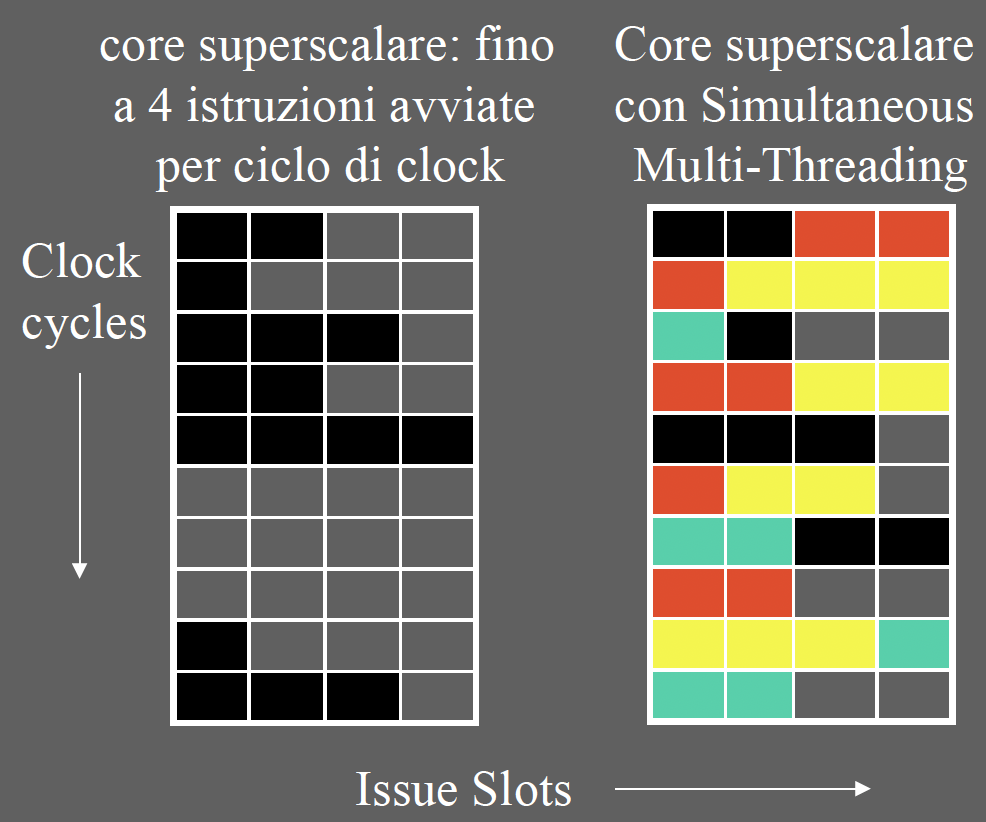
\includegraphics[width=0.8\textwidth]{images/core_smt.png}
    \caption{Esecuzione parallela con SMT: istruzioni di diversi thread (colori diversi) avviate simultaneamente.}
\end{figure}

\nt{(Per questa immagine) Ad ogni ciclo di clock il core può eseguire istruzioni di peer-thread diversi, ma con un massimo di 2 peer-thread per core.}

\subsection{Definizioni: Dual-Threaded vs Dual-Core}

L'introduzione del \textbf{Simultaneous Multi-Threading} può generare confusione nella terminologia:

\begin{itemize}
    \item Un \textbf{core dual-threaded} è un singolo core capace di eseguire contemporaneamente istruzioni appartenenti a due o più \textbf{peer thread}.
    \item Un \textbf{dual-core} è un processore con due core fisici distinti, ciascuno capace di eseguire istruzioni di processi distinti in parallelo. 
\end{itemize}

\nt{Ogni core di un dual-core può essere a sua volta multi-threaded, combinando le capacità di esecuzione parallela di thread e processi.}


\section{Ma l'SMT è sempre vantaggioso?}
\textbf{Si}: ecco lo speed-up ottenuto su uno dei core di una CPU i7 nel passare da un solo thread a 2, per diversi benchmarks.\\
Il dato “Energy efficiency” ci dice se l’introduzione dell’SMT è vantaggiosa dal punto di vista dell’energia consumata. Un valore superiore a 1.0 significa che l’SMT riduce il tempo di esecuzione più di quanto aumenti i consumi.
\begin{figure}[h] \centering 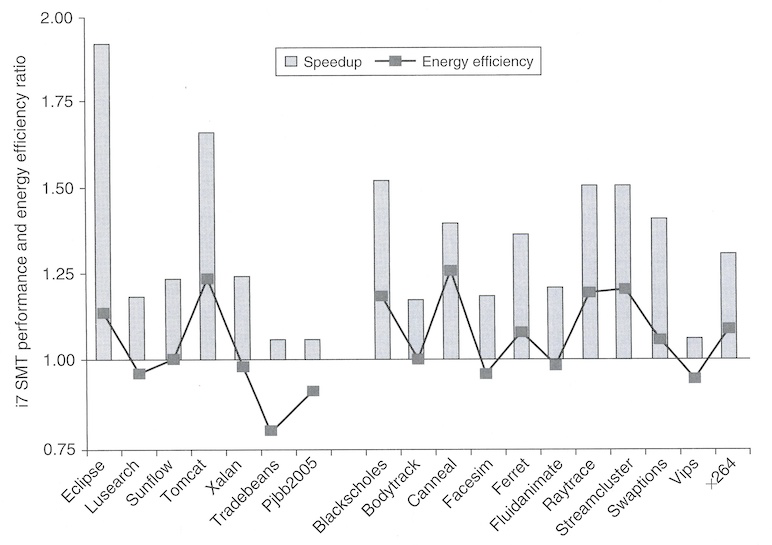
\includegraphics[width=0.50\linewidth]{images/smt_benchmark.png} \caption{smt_benchmark} \end{figure}

\qs{difficile}{ Nessuna CPU implementa una forma di Simultaneous Multi-Processing, in cui cioè istruzioni appartenenti a processi diversi vengono eseguite in parallelo all’interno dello stesso core. Perché?}
\nt{Due processi non condividono lo stesso spazio di indirizzamento, quindi non condiviono la stessa tabella delle pagine .\\
    Invece i peer-thread di un task multi-threaded condividono lo spazio di indirizzamento, quindi possono essere eseguiti in parallelo all’interno dello stesso core.}



\afterpage{}
\chapter{Scheduling della CPU}
\section{Scheduling}
\subsection{Fasi di eleborazion e di I/O}
Durante la vita di un processo, si alternano fasi di uso della \textbf{CPU} (CPU burst) e fasi di attesa per il completamento di operazioni di \textbf{I/O} (I/O burst). 

Possiamo distinguere due categorie di processi:

\begin{itemize}
    \item \textbf{Processi CPU-bound:} usano intensamente la CPU e interagiscono poco con i dispositivi di I/O (ad esempio un compilatore).
    \item \textbf{Processi I/O-bound:} usano poco la CPU ma fanno ampio uso dei dispositivi di I/O (ad esempio un editor o un browser).
\end{itemize}


\subsection{Lo Scheduler della CPU}
Consideriamo la situazione in cui un processo utente abbandona la \textbf{CPU}. Il Sistema Operativo (SO) si "sveglia" e deve decidere a quale, fra i processi in \textbf{Coda di Ready} (processi \emph{ready to run}), assegnare la CPU. Questa operazione è detta \textbf{Scheduling della CPU}, e viene gestita dal modulo del SO detto \textbf{scheduler}.

Quando interviene lo scheduler per scegliere il successivo processo a cui assegnare la CPU? Possiamo considerare quattro situazioni, che ci porteranno a definire i concetti di \textbf{scheduling con} e \textbf{senza diritto di prelazione}:

\begin{enumerate}

    \item Il processo che sta usando la CPU passa volontariamente dallo stato di running allo stato di waiting.
    \item Il processo che sa usando la CPU termina.
    \begin{itemize}
        \item In questi \textbf{due casi}, lo scheduler deve prendere un processo dalla coda di readt e mandarlo in eseucuzione
        \item \nt{Un sistema operativo che intervenga nei casi 1 e 2 è sufficiente per implementare il multi-tasking}
        \item \qs{}{Che succede se mandiamo in eseucuzione un programma che contiene una istruzione del tipo \texttt{while(true) printf("who's carr?")};}
        \item Il \textbf{SO} deve poter intervenire in modo da evitare che un processo si simpossessi della CPU, quindi...
    \end{itemize}
    \item Il processo che sta usando la CPU viene obbligato a passare dallo stato di running allo stato di ready
    \begin{itemize}
        \item Il passaggio non avviene mai \textbf{volontariamente}, il processo non vorrebbe lasciare la CPU a favore di qualcun'altro.
        \item Nei sistemi time sharing il SO non perde \textbf{mai} completamente il controllo del sistema
        \item Il SO mantiene il controllo della CPU attraverso un timer hardware, allo scadere del timer il controllo della CPU verrà restituito al SO, che sceglierà un processo dalla RQ un processo da mandare in esecuzione.
    \end{itemize}
    \item Un processo Px entra in coda di ready arrivando da una coda di wait oppure perchè è appena stato lanciato. 
    \qs{}{Perchè il SO interviene in questo caso?}
    \begin{itemize}
    \item \textbf{Primo:} i processi non si spostano autonomamente da una coda all’altra. È il Sistema Operativo (SO) che gestisce i loro \textbf{PCB} (Process Control Block). Ad esempio, quando il SO si accorge del completamento di un'operazione di I/O per cui il processo $P_x$ era in attesa, interviene per spostare (il PCB di) $P_x$ dalla \textbf{coda di wait} alla \textbf{coda di ready}.
    
    \item \textbf{Secondo:} se il processo $P_x$ risulta più "importante" rispetto al processo attualmente in esecuzione, il SO può decidere di togliere quest’ultimo dalla \textbf{CPU} e mandare in esecuzione $P_x$.
\end{itemize}
\end{enumerate}
Quando un sistema interviene solo nei casi 1 e 2 si parla di: \textbf{Scheduling senza (diritto di) prelazione}.\\
Quando un sistema interviene anche nei casi 3 e 4 si parla di: \textbf{Scheduling con (diritto di) prelazione}\\
Chiaramente, lo \textcolor{blue}{\textbf{scheduling preemptive}} è più sicuro per gli utenti, ma la sua implementazione richiede un \textcolor{purple}{sistema operativo} e un’\textcolor{purple}{architettura hardware} più sofisticati (ad esempio, un \textbf{timer dedicato}).\\
I moderni \textbf{sistemi operativi general purpose} usano tutti una qualche variante di \textcolor{blue}{\textbf{scheduling preemptive}}. Tuttavia, per applicazioni specifiche può essere sufficiente uno \textcolor{red}{\textbf{scheduling non-preemptive}}, permettendo l'uso di sistemi operativi più semplici e leggeri.\\
Lo \textcolor{blue}{\textbf{scheduling preemptive}} può portare a situazioni che necessitano di essere gestite con attenzione. Ad esempio, consideriamo un processo che deve compiere un’operazione di \textcolor{orange}{\textbf{I/O}} e chiama la relativa \textcolor{purple}{system call}. Il controllo viene trasferito al \textcolor{purple}{sistema operativo}, che inizia l’operazione per conto del processo utente. Nel frattempo, scade il timer e il controllo viene passato a un'altra porzione del codice del \textcolor{purple}{SO}.\\
Di conseguenza, una operazione delicata (altrimenti non sarebbe stata gestita dal \textcolor{purple}{SO}) viene interrotta a metà, e le \textcolor{orange}{\textbf{strutture dati}} potrebbero trovarsi in uno stato inconsistente poiché la system call di \textcolor{orange}{\textbf{I/O}} non ha finito di aggiornarle.\\
\qs{}{Cosa succede se ora la \textcolor{purple}{CPU} viene data a un altro processo utente che tenta di usare lo stesso dispositivo di \textcolor{orange}{\textbf{I/O}} che il processo precedente stava utilizzando? Quale semplice soluzione può essere adottata in tali casi?}
\nt{Vogliamo che il processo riesca a completare la richiesta al controller dell'I/O, niente di più}.
Mentre \textbf{Unix} è stato sviluppato fin dall’inizio come sistema di tipo {\textbf{preemptive}}, nei sistemi \textbf{Microsoft} la preemption è stata introdotta solo con \textbf{Windows 95}. Questo è dovuto al fatto che i sistemi operativi della famiglia \textbf{MS-Dos} sono nati come sistemi {\textbf{mono-utente}}, per i quali era sufficiente un sistema operativo più semplice. Inoltre, i primi sistemi per PC giravano su {CPU} semplici ed economiche, non dotate del supporto hardware necessario per implementare un sistema operativo {\textbf{preemptive}}.\\

\subsection{Il Dispatcher}
Quando lo scheduler ha scelto il processo a cui assegnare la CPU, interviene un altro modulo del SO, il \textit{dispatcher}, che:
\begin{itemize}
    \item Effettua l'operazione di \textit{context switch}.
    \item Effettua il passaggio del sistema in \textit{user mode}.
    \item Posiziona il \textit{PC} della CPU alla corretta locazione del programma da far ripartire.
\end{itemize}

Si definisce \textbf{Dispatch latency} il tempo impiegato per effettuare la commutazione da un processo ad un altro.

\section{Criteri di Scheduling}
Come abbiamo visto, lo scheduler della CPU interviene per assicurare il corretto funzionamento del sistema. Tuttavia, quando lo scheduler deve mandare in esecuzione un processo, quale criterio usa per scegliere tra tutti i processi presenti nella coda di ready? 

Si possono prendere in considerazione diversi obiettivi:

- Massimizzare l’\textbf{utilizzo} della CPU nell’unità di tempo, anche se questo dipende dal carico.
- Massimizzare il \textbf{throughput}, ossia la produttività del sistema, che si misura come il numero di processi completati in media in una certa unità di tempo.
- Minimizzare il \textbf{tempo di risposta}, cioè il tempo che intercorre da quando si avvia un processo a quando questo inizia effettivamente ad eseguire. Questo aspetto è particolarmente importante per i sistemi interattivi.

- Minimizzare il \textit{Turnaround time}: ossia il tempo medio di completamento di un processo, che va da quando entra per la prima volta nella \textit{ready queue} a quando termina.
- Minimizzare il \textit{Waiting time}: ossia la somma del tempo trascorso dal processo in \textit{ready queue}, ovvero quando il processo è pronto per eseguire il suo codice ma la CPU è occupata da un altro processo.

\qs{}{Che relazione c'è tra waiting time e turnaround time?}
\nt{Turnaround time - waiting time = tempo di esecuzione}

\section{Algoritmi di Scheudling}
\begin{itemize}
    \item \textbf{First Come, First Served (FCFS)}: Scheduling per ordine di arrivo.
    \item \textbf{Shortest Job First (SJF)}: Scheduling per brevità.
    \item \textbf{Priority Scheduling}: Scheduling per priorità.
    \item \textbf{Round Robin (RR)}: Scheduling circolare.
    \item \textbf{Multilevel Queue}: Scheduling a code multiple.
    \item \textbf{Multilevel Feedback Queue}: Scheduling a code multiple con retroazione.
\end{itemize}

\noindent \textbf{Nota Bene}: Nel seguito, considereremo processi con un unico \textit{burst} di CPU, senza \textit{burst} di I/O e con una durata espressa in generiche unità di tempo. Questo semplifica la comprensione degli algoritmi senza perdita di generalità.

\subsection{First Come First Served (FCFS)}
L'algoritmo \textit{First Come, First Served (FCFS)} è facile da implementare: gestisce la \textit{ready queue} (RQ) in modo FIFO (\textit{First In, First Out}). 
\begin{itemize}
    \item Il \textit{PCB} di un processo che entra nella \textit{RQ} viene inserito in fondo alla coda.
    \item Quando la CPU si libera, viene assegnata al processo il cui \textit{PCB} si trova in testa alla coda FIFO.
\end{itemize}

\noindent FCFS è un algoritmo non \textit{preemptive}, per cui non è adatto per i sistemi \textit{time-sharing}. Inoltre, con FCFS, il tempo di attesa per il completamento di un processo può risultare spesso molto lungo.

\subsubsection{Esempio}
Consideriamo tre processi che arrivano assieme al tempo t=0, e che entrano in CPU nell’ordine P1, P2, P3.
Come abbiamo già detto, i tre processi eseguono per un unico burst di CPU, e poi terminano.
\begin{table}[h]
    \centering
    \begin{tabular}{|c|c|}
        \hline
        \textbf{Process} & \textbf{Burst Time} \\
        \hline
        $P_1$ & 24 \\
        $P_2$ & 3 \\
        $P_3$ & 3 \\
        \hline
    \end{tabular}
    \caption{Process and Burst Time}
    \label{tab:process_burst_time}
\end{table}

Usiamo un diagramma di Gnatt per rappresentare questa situazione
\begin{figure}[h]
    \centering
    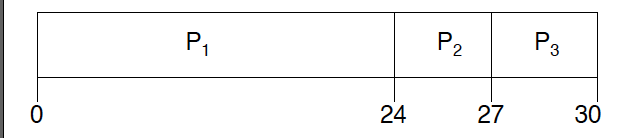
\includegraphics[width=0.5\linewidth]{images/FCFS_gnatt.png}
\end{figure}
Tempi di attesa $P_1 = 0; P_2 = 24; P_3 = 17$\\
Tempo medio di attesa $(0+24+27)/3 = 17$\\
Si dice che si è verificato \textbf{effetto convoglio}; i job più corti si sono dovuti accodare a quello lungo.
\bigskip
Se invece supponiamo che l'ordine di arrivo sia: P2, P3, P1
Tempi di attesa $P_1 = 6; P_2 = 0; P_3 = 3$\\
Tempo medio di attesa $(6+0+3)/3 = 3 \longleftrightarrow$ Molto meglio del caso precedente!\\

\subsubsection{Osservazioni}
Dunque, l'algoritmo \textit{FCFS} sembra comportarsi male nei confronti dei processi brevi. \\
Inoltre, \textit{FCFS} è pessimo per i sistemi \textit{time-sharing} poiché non garantisce un tempo di risposta ragionevole.\\
Ancora peggio, \textit{FCFS} non è adatto ai sistemi \textit{real-time} perché non è \textit{preemptive}.\\\\
Dall’esempio visto, sembra che le prestazioni migliorino facendo eseguire prima i processi più corti, indipendentemente dall’ordine di arrivo nella \textit{ready queue}. Tuttavia, questo apre la porta a nuovi problemi, che andremo a considerare.

\subsection{Shortest Job First (SJF)}
Si esamina la durata del prossimo \textit{burst} di CPU di ciascun processo in \textit{RQ} e si assegna la CPU al processo con il \textit{burst} di durata minima.\\
Il nome esatto di questo algoritmo è \textit{Shortest Next CPU Burst}.\\
 Può essere usato in modalità \textit{pre-emptive} e \textit{non pre-emptive}.\\
Nel caso \textit{preemptive}, se arriva in \textit{ready queue} un processo il cui \textit{burst time} è inferiore al tempo rimanente del processo attualmente in esecuzione, quest'ultimo viene interrotto e la CPU passa al nuovo processo. Questo schema è noto come \textit{Shortest-Remaining-Time-First} (SRTF).\\
\subsubsection{Esempio}
\begin{table}[ht]
    \centering
    \begin{tabular}{|c|c|c|}
        \hline
        \rowcolor[gray]{0.6} 
        Process & Arrival Time & Burst Time \\
        \hline
        $P_1$ & 0 & 7 \\
        $P_2$ & 2 & 4 \\
        $P_3$ & 4 & 1 \\
        $P_4$ & 5 & 4 \\
        \hline
    \end{tabular}
    \caption{Process, Arrival Time, and Burst Time}
    \label{tab:process_times}
\end{table}

\subsubsection{Non-preemptive}
Esempio:
\begin{figure}[ht]
    \centering
    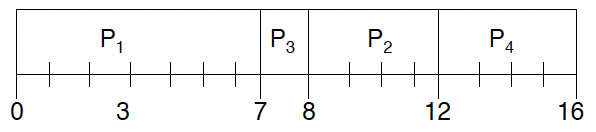
\includegraphics[width=0.2\linewidth]{images/SJF_nonpreemptive.png}
    \caption{Average waiting time $(0 + 6 + 3 + 7)/4 = 4$}
\end{figure}

\subsubsection{preemptive}
Esempio:
\begin{figure}[ht]
    \centering
    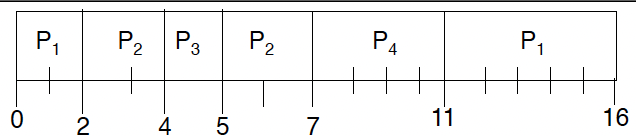
\includegraphics[width=0.2\linewidth]{images/SJF_preemptive.png}
    \caption{Average waiting time $(9 + 1 + 0 + 2/4 = 3$}
\end{figure}


\subsection{Osservazioni}
Si può dimostrare che l'algoritmo \textit{Shortest Job First} (SJF) è ottimale: spostando un processo breve prima di uno di lunga durata (anche se quest’ultimo è arrivato prima) si migliora l'attesa del processo breve più di quanto si peggiori quella del processo lungo. Di conseguenza, il tempo medio di attesa diminuisce, così come il \textit{turnaround time}.

SJF è ottimale: nessun altro algoritmo di \textit{scheduling} può produrre un tempo di attesa medio e un \textit{turnaround time} medio migliori. Tuttavia, c'è un problema...\\
Purtroppo, la durata del prossimo burst di CPU di un processo non è nota, il che rende l'algoritmo \textit{Shortest Job First} (SJF) non implementabile nella sua forma pura. SJF può al massimo essere approssimato utilizzando medie pesate per stimare la durata del prossimo burst di CPU di un processo, basandosi sulla durata dei burst di CPU precedenti.\nt{Da rivededere!!!!}\\

Lo \textit{scheduling} viene quindi eseguito sulla base di queste stime, fatte per tutti i processi nella \textit{Ready Queue} in un dato momento.\\
In sostanza, il \textit{First Come, First Served} (FCFS) è il peggiore degli algoritmi ragionevoli: funziona, ma spesso fornisce tempi medi di attesa e di \textit{turnaround} pessimi.\\

Al contrario, lo \textit{Shortest Job First} (SJF) è il migliore algoritmo possibile, ma non è implementabile nella pratica, e possiamo solo usarlo per fare simulazioni con processi i cui burst di CPU siano noti a priori.\\

FCFS e SJF rappresentano i due estremi di uno spettro di possibili algoritmi di \textit{scheduling}. Un algoritmo di \textit{scheduling} sarà tanto migliore quanto più le sue prestazioni si allontanano da quelle di FCFS e si avvicinano a quelle di SJF.

\subsection{Scheduling a Priorità}
SJF è un tipo scheduling a priorità, la durata del prossimo burst time è la priorità corrente di ogni processo.
FCFS è uno scheduling a priorità, viene data più alta ai primi che arrivano
In generale, il calcolo della priorità dei processi può essere:
\begin{itemize}
    \item \textbf{Interna al sistema}: calcolata dal SO sulla base del comportamento di ogni processo (ad esempio, in base alle risorse usate fino a quel momento da un processo).
    \item \textbf{Esterna al sistema}: assegnata con criteri esterni al SO (ad esempio, una priorità che cambia in base a quale utente ha lanciato il processo).
\end{itemize}

Lo \textit{scheduling} a priorità può essere implementato sia in modalità \textbf{preemptive} che \textbf{non preemptive}.

\subsubsection{Starvation e aging}
\qs{Problema}{Che succede se un processo in RQ ha sempre una priorità peggiore di qualche altro processo in RQ?}
Il processo potrebbe non essere mai scelto dallo scheduler. Questo fenomeno è noto come \textbf{starvation} (muore di fame...). 

Per risolvere il problema della \textit{starvation}, si usa un meccanismo chiamato \textbf{aging}: il SO aumenta progressivamente la priorità di un processo $P_x$ man mano che $P_x$ passa tempo nella Ready Queue (RQ). In questo modo, prima o poi, $P_x$ avrà una priorità maggiore rispetto agli altri processi e verrà scelto dallo scheduler.

\qs{}{Gli algoritmi \textit{FCFS}, \textit{SJF preemptive} e \textit{non preemptive} possono provocare starvation?}
\nt{Per SJF, arrivano sempre processi con burst piccolissimi e quindi un processo più grande aspetterà (Sia per preemptive che non)}

\subsection{Scheduling Round Robin (RR)}
Ogni processo ha a disposizione una certa quantità di tempo di CPU, chiamata \textbf{quanto di tempo} (valori ragionevoli vanno da 10 a 100 millisecondi). Per ora, assumiamo un unico quanto di tempo prefissato assegnato a tutti i processi. 

Se entro questo arco di tempo il processo non lascia volontariamente la CPU, viene interrotto e rimesso nella Ready Queue (RQ). La RQ è vista come una coda circolare, e si verifica una sorta di \textit{“girotondo”} di processi.

L'implementazione dello scheduling \textbf{round robin} è concettualmente molto semplice:
\begin{itemize}
    \item Lo scheduler sceglie il primo processo in RQ (ad esempio secondo un criterio FCFS).
    \item Lancia un timer inizializzato al quanto di tempo.
    \item Passa la CPU al processo scelto.
\end{itemize}

Se il processo ha un CPU burst minore del quanto di tempo, il processo rilascierà la CPU volontariamente prima dello scadere del tempo assegnatogli. Se invece il CPU burst del processo è maggiore del quanto di tempo, allora:
\begin{itemize}
    \item Il timer scade e invia un interrupt.
    \item Il SO riprende il controllo della CPU.
    \item Togliere la CPU al processo in esecuzione e metterlo in fondo alla RQ.
    \item Prendere il primo processo in RQ e ripetere tutto.
\end{itemize}

\subsubsection{Osservazioni}
Se ci sono \( n \) processi in coda ready e il quanto di tempo è \( q \), allora ogni processo riceve \( \frac{1}{n} \) del tempo della CPU e nessun processo aspetta per più di \( (n-1)q \) unità di tempo.

Il \textbf{Round Robin} è l'algoritmo di scheduling naturale per implementare il time sharing ed è quindi particolarmente adatto per i sistemi interattivi: nel caso peggiore, un utente non aspetta mai più di \( (n-1)q \) unità di tempo prima che il suo processo venga servito.

Come vedremo negli esempi di casi reali, il SO adotta poi ulteriori misure per migliorare il tempo di risposta dei processi interattivi.

\subsection{Esempio}
\begin{table}[h]
    \centering
    \begin{tabular}{|c|c|}
        \hline
        \textbf{Process} & \textbf{Burst Time} \\
        \hline
        $P_1$ & 53 \\
        $P_2$ & 17 \\
        $P_3$ & 68 \\
        $P_4$ & 24 \\
        \hline
    \end{tabular}
    \caption{Process and Burst Time}
    \label{tab:process_burst_time}
\end{table}
\begin{figure}[h]
    \centering
    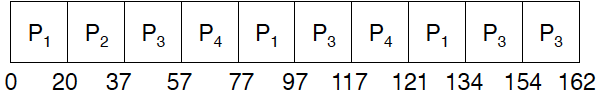
\includegraphics[width=0.25\linewidth]{images/RR_20.png}
\end{figure}
Tipicamente sia ha un \textit{turnaround} medio maggiore di SJF, ma un migliore \textbf{tempo di risposta}
Le prestazioni del \textbf{Round Robin} dipendono molto dal valore del quanto di tempo \( q \) scelto:
\begin{itemize}
    \item \( q \) tendente a infinito rende \textbf{RR} uguale a \textbf{FCFS}.
    \item \( q \) tendente a zero produce un maggior effetto di “parallelismo virtuale” tra i processi.
    \item Tuttavia, questo aumenta il numero di context switch e, di conseguenza, l'overhead.
\end{itemize}

\subsection{Scheduling a Code Multiple}

I processi possono essere suddivisi in classi differenti:
\begin{itemize}
    \item \textbf{foreground}: processi interattivi (es. un editor)
    \item \textbf{background}: processi che non interagiscono con l'utente
    \item \textbf{batch}: processi la cui esecuzione può essere differita
\end{itemize}

La risorsa di esecuzione (RQ) può essere partizionata in più code:
\begin{itemize}
    \item I processi vengono inseriti in una coda basata sulle loro proprietà
    \item Ogni coda viene gestita con lo scheduling appropriato
\end{itemize}
Ogni coda ha quindi la sua politica di scheduling, ad esempio:
\begin{itemize}
    \item \textit{foreground}: \textbf{RR}
    \item  \textit{background e batch}: \textit{FCFS}
\end{itemize}
\qs{}{Ma come si sceglie fra le code?
\begin{itemize}
    \item \textbf{Scheduling a priorità fissa}: servire prima tutti i processi nella coda foreground e poi quelli in background e batch. Possibilità di \textbf{starvation}.
    \item  \textbf{Time slice}: ogni coda ha una certa quantità di tempo di CPU, ad esempio: 80\% alla coda foreground e 20\% alla coda background e batch
\end{itemize}
}

\begin{figure}[h]
    \centering
    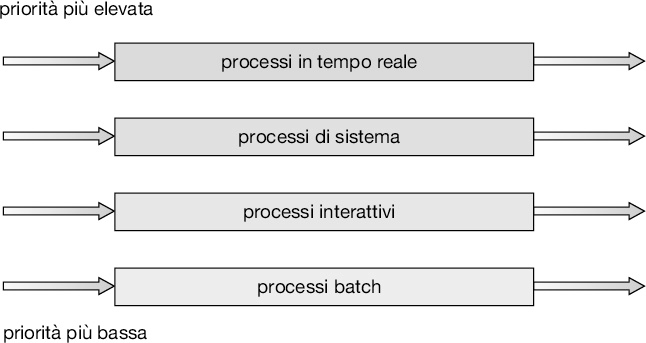
\includegraphics[width=0.5\linewidth]{images/Scheduling_multiple_queue.png}
    \caption{Partizionamento dei processi in più code}
\end{figure}

\subsection{Scheduling a Code Multilivello con retroazione (MFQS)}
Il tipo più generale di algoritmo di scheduling è lo \textbf{scheduling a code multilivello con retroazione} (MFQS), utilizzato dai sistemi operativi moderni.

\begin{itemize}
    \item L'assegnamento di un processo a una coda non è fisso: i processi possono essere spostati dal SO per adattarsi alla lunghezza del loro \textit{CPU burst}.
    \item Ogni coda è gestita con lo scheduling più adatto ai processi in essa contenuti.
\end{itemize}

Esempio (fig. 5.4):
\begin{figure}[h]
    \centering
    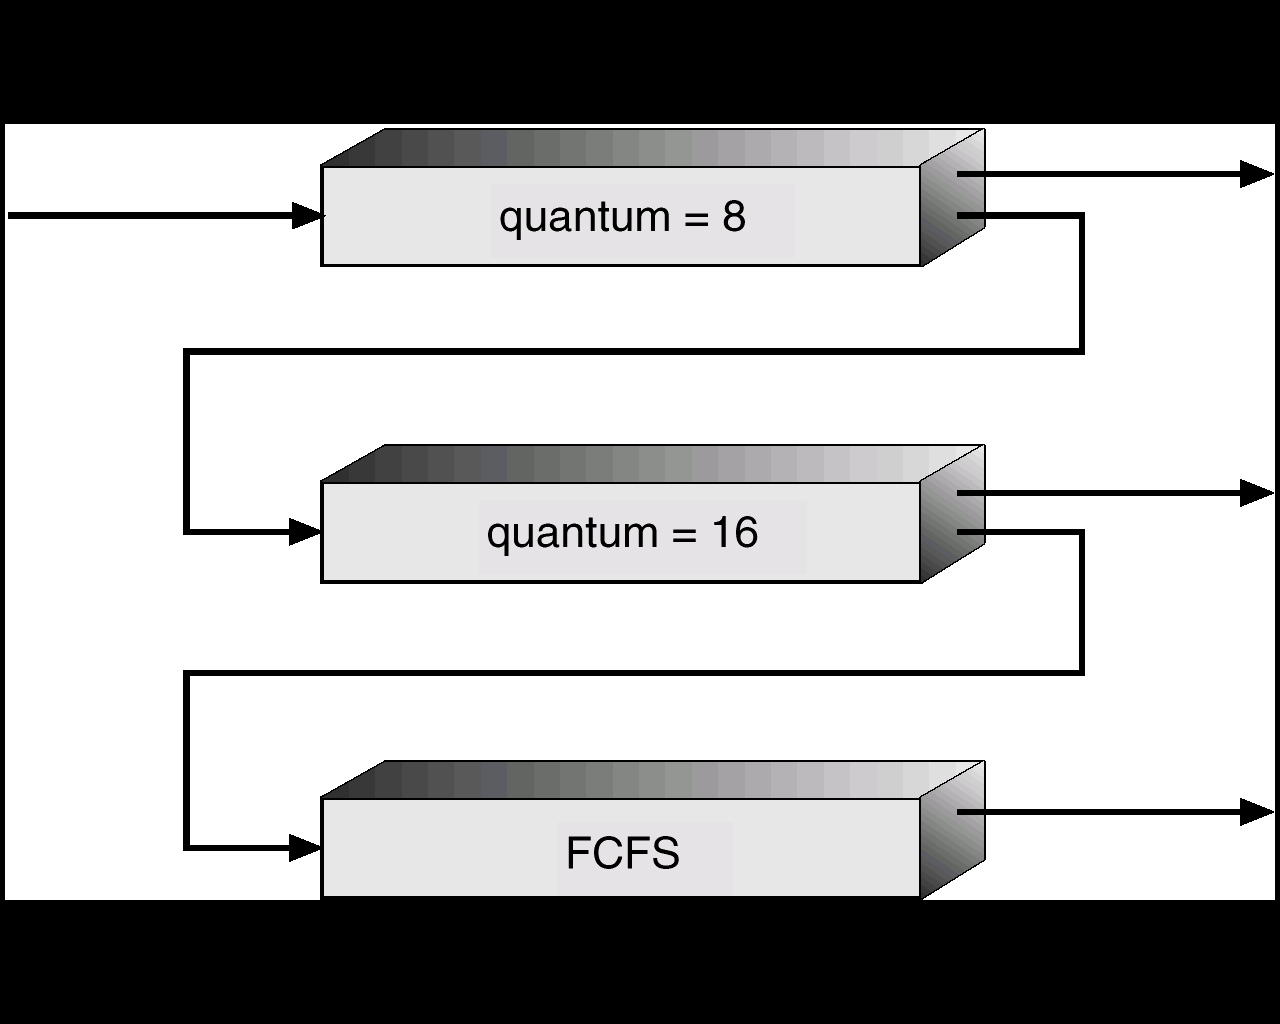
\includegraphics[width=0.25\linewidth]{images/MFQS.png}
    \caption{Esempio di MFQS}
    \label{fig:5.4}
\end{figure}
\begin{itemize}
    \item Le prime due code sono gestite con \textit{Round Robin (RR)}, mentre la terza con \textit{First-Come, First-Served (FCFS)}.
    \item Quando un processo nasce, è inserito nella prima coda ($q=8$). Se non finisce il \textit{CPU burst} entro il quanto, viene retrocesso alla coda successiva.
    \item È definita una priorità tra le code, che sono gestite con \textit{preemption}.
\end{itemize}

La politica MFQS è caratterizzata da:
\begin{itemize}
    \item numero di code
    \item algoritmo di scheduling per ogni coda
    \item quando declassare o promuovere un processo
    \item in che coda inserire un processo quando arriva (dall'esterno o da un \textit{I/O burst})
\end{itemize}

MFQS è il tipo di scheduling più generale e complesso da configurare.


\section{Scheduling per sistemi multi-core}
Sono ormai comuni le architetture con CPU a 2, 4, 8 core, Sono, in sostanza, dei piccoli sistemi multiprocessore in cui sullo stesso chip sono presenti due o più core che vedono la stessa memoria principale e condividono un livello di cache.
La presenza di più “unità di esecuzione” dei processi, permette naturalmente di aumentare le prestazioni della macchina, posto che il SO sia in grado di sfruttare a pieno ciascun core.

I sistemi operativi moderni prevedono la \textbf{multielaborazione simmetrica} (SMP), in cui uno scheduler gira su ciascun core.
\begin{itemize}
    \item I processi "ready to run" possono essere inseriti in una coda comune oppure in una coda separata per ogni core.
    \item Lo scheduler di ciascun core sceglie un processo dalla propria coda e lo manda in esecuzione.
\end{itemize}

Un aspetto chiave nei sistemi multi-core è il \textbf{bilanciamento del carico}, ossia la distribuzione omogenea dei processi tra i core.
\begin{itemize}
    \item Con una coda comune, il bilanciamento è automatico: un core inattivo prende un processo dalla coda comune.
    \item Con code separate per ogni core, è necessario un meccanismo per spostare i processi dai core sovraccarichi a quelli scarichi. \textbf{Questo è il processo preferito dai moderni SO}
    \item Ad esempio, Linux SMP attiva il bilanciamento del carico ogni 200 ms o quando una coda si svuota.
\end{itemize}

Spostare un processo tra core può causare rallentamenti dovuti alla \textbf{cache}, poiché il processo potrebbe non trovare i dati nelle cache private del nuovo core.
Non trovandoli è costretto a spendere più tempo per recuperarli, se va bene, dalla cache L3, che condivide con gli altri core. Per evitare questo problema, specifiche \textit{system call} permettono di vincolare un processo a un certo core.

\subsection{Esempio}

\begin{figure}[h]
    \centering
    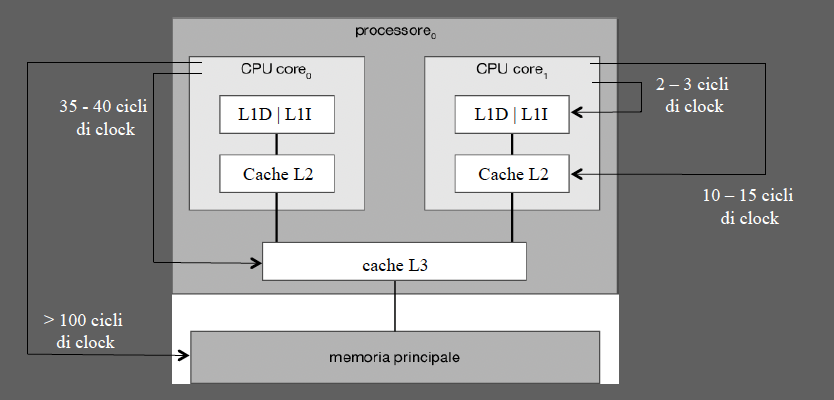
\includegraphics[width=0.5\linewidth]{images/Scheduling_multi_core_i7.png}
    \caption{Scheduling example}
    \label{fig:schedi7}
\end{figure}
Qui vediamo il costo in cicli di clock necessari per accedere ad un dato/istruzione in un certo livello di cache. I valori si riferiscono ad un processore Intel core i7, ma valgono per la maggior parte dei processori moderni \ref{fig:schedi7}.

\section{Esempi di sistemi operativi}
Solaris utilizza uno \textbf{scheduling a priorità con code multiple a retroazione}, suddividendo i processi in 4 classi:
\begin{enumerate}
    \item real time (priorità maggiore)
    \item sistema
    \item interattiva
    \item time sharing (priorità minore)
\end{enumerate}

\begin{itemize}
    \item Un processo usa la CPU fino a quando non termina, va in \textit{wait}, esaurisce il quanto di tempo o è preemptato.
    \item I processi delle classi \textit{time sharing} e \textit{interattiva} hanno criteri di scheduling simili con 60 livelli di priorità.
    \item La priorità di un processo e il quanto di tempo assegnato sono inversamente proporzionali. Se un processo esaurisce il quanto, la sua priorità viene abbassata; al contrario, se si sospende prima, la priorità aumenta.
\end{itemize}

Il comportamento del processo stabilisce se rientra nella classe \textit{time sharing} (priorità 0-49) o \textit{interattiva} (priorità 50-59)
% Requires: \usepackage{colortbl}
\begin{table}[h]
    \centering
    \begin{tabular}{|c|c|c|c|}
    \hline
    \rowcolor{gray} \textbf{Priorità corrente} & \textbf{Quanto di tempo} & \textbf{Nuova priorità} & \textbf{Nuova priorità} \\
    \rowcolor{gray} & \textbf{(millisecondi)} & \textbf{(quanto esaurito)} & \textbf{(quanto non esaurito)} \\
    \hline
    0 & 200 & 0 & 50 \\
    \hline
    20 & 120 & 10 & 52 \\
    \hline
    30 & 80 & 25 & 53 \\
    \hline
    59 & 20 & 49 & 59 \\
    \hline
    \end{tabular}
    \caption{Tabella delle priorità e tempi}
    \label{tab:pri_tempi}
\end{table}

La \textbf{priorità corrente} di un processo determina il \textbf{quanto di tempo} che gli viene assegnato. Priorità e tempo assegnato sono inversamente proporzionali.

\begin{itemize}
    \item \textbf{Quanto esaurito}: se un processo ha esaurito tutto il quanto di tempo senza sospendersi, la sua nuova priorità sarà più bassa, e in futuro riceverà un quanto di tempo più lungo.
    \item \textbf{Quanto non esaurito}: se un processo si sospende prima di consumare tutto il quanto, la sua nuova priorità sarà più alta, e in futuro riceverà un quanto di tempo più breve.
\end{itemize}


\begin{itemize}
    \item I processi \textit{real time} e di \textit{sistema} hanno priorità fissa, superiore a quella delle classi \textit{time sharing} e \textit{interattiva}.
    \item Lo scheduler assegna la CPU al processo con la priorità globale più alta e, in caso di parità, utilizza il \textit{Round Robin} (RR).
    \item L'algoritmo è \textbf{preemptive}: un processo attivo può essere interrotto da uno con priorità globale più alta.
\end{itemize}

\subsection{Lo scheduling in Windows}
Lo scheduling in Windows è basato su \textbf{priorità con retroazione e prelazione}, utilizzando 32 livelli di priorità:
\begin{itemize}
    \item I processi \textit{real-time} hanno priorità da 16 a 31.
    \item I processi non real-time hanno priorità da 1 a 15, con 0 riservato.
\end{itemize}

Per i processi non real-time:
\begin{itemize}
    \item Quando un processo nasce, ha una priorità iniziale di 1.
    \item Lo scheduler assegna la CPU al processo con la priorità più alta, usando \textit{Round Robin} (RR) in caso di parità.
    \item Se un processo va in \textit{wait} prima di esaurire il quanto di tempo, la sua priorità viene aumentata (fino a 15), a seconda dell'evento in attesa (maggiore incremento per input da tastiera, minore per I/O da disco).
    \item Se un processo esaurisce il quanto di tempo, la sua priorità viene abbassata, ma mai sotto 1.
\end{itemize}

Questa strategia favorisce i processi interattivi (mouse e tastiera) per migliorare il \textbf{tempo di risposta}. Inoltre, quando un processo passa in \textit{foreground}, il suo quanto di tempo viene moltiplicato per 3, consentendogli di mantenere la CPU per un periodo più lungo.

\subsection{Lo Scheduling in Linux}
Dal 2007, Linux utilizza il \textbf{Completely Fair Scheduler} (CFS) come algoritmo di scheduling predefinito.

Il CFS distribuisce equamente il tempo di CPU tra i processi \textit{ready to run}, seguendo l'assunzione che se ci sono $N$ processi attivi, ciascun processo dovrebbe ricevere esattamente $\frac{1}{N}$ del tempo di CPU.

Ad ogni \textit{context switch}, il CFS ricalcola per quanto tempo assegnare la CPU a un processo $P$, in modo che tutti abbiano la stessa quantità di tempo CPU. Siano:
\begin{itemize}
    \item $P.\texttt{expected\_run\_time}$: il tempo di CPU spettante a $P$;
    \item $P.\texttt{vruntime}$: il tempo di CPU già consumato da $P$;
    \item $P.\texttt{due\_cputime}$: il tempo di CPU che ancora spetta a $P$.
\end{itemize}

Dunque:
\[
P.\texttt{vruntime} = P.\texttt{expected\_run\_time} - P.\texttt{due\_cputime}
\]
La CPU viene assegnata al processo con il valore più basso di $P.\texttt{vruntime}$, ossia al processo che ha usato meno CPU fino a quel momento.

Nel CFS, i processi \textit{ready to run} non sono organizzati in code di scheduling, ma come nodi in un \textbf{red-black tree (R-B tree)}, che consente operazioni di ricerca, inserimento e cancellazione con complessità computazionale $O(\log n)$, dove $n$ è il numero di nodi.

Negli alberi R-B il nodo più a sinistra è sempre quello col valore chiave più basso, e nel CFS i processi sono inseriti nel R-B tree usando come chiave P.vruntime.
Dunque, il processo associato al nodo più a sinistra ha il valore P.vruntime più basso, cioè è il processo che ha usato la CPU per meno tempo, e al context switch sarà scelto per entrare in esecuzione.

\begin{figure}
    \centering
    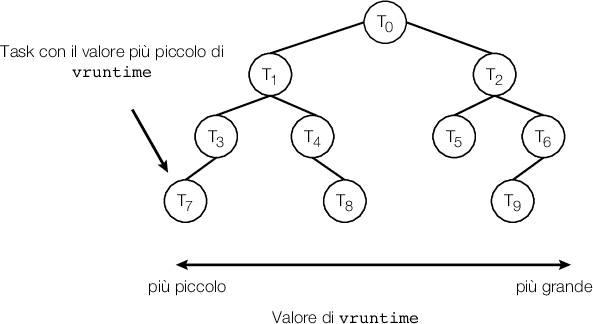
\includegraphics[width=0.5\linewidth]{images/Scheduling-Linux-Tree.png}
    \caption{vrun time tree}
    \label{fig:v-runtimetree}
\end{figure}

\afterpage{}

\chapter{Sincronizzazione dei Processi}

\section{Introduzione}
Più processi possono cooperare per compiere un determinato lavoro, e spesso \textbf{condividono dei dati}.

\begin{itemize}
    \item È fondamentale che l'accesso ai dati condivisi da parte dei vari processi non produca dati inconsistenti.
    \item I processi cooperanti devono quindi \textbf{sincronizzarsi} per accedere ai dati condivisi in modo ordinato.
    \item \textbf{Problema}: mentre un processo $P$ sta elaborando dati condivisi, il SO potrebbe toglierlo dalla CPU in qualsiasi momento. Altri processi non devono poter accedere ai dati condivisi finché $P$ non ha completato l'elaborazione.
\end{itemize}

\subsection{Esempio: Produttore-Consumatore con n eleemnti}
Usiamo una variabile \textbf{\textit{condivisa}} \textbf{counter} inizializzata a 0 che indica il numero di elementi nel buffer.

I due programmi sono corretti se considerati separatamente, ma possono non funzionare quando vengono eseguiti insieme.

\begin{itemize}
    \item Il problema risiede nell'uso della variabile condivisa \texttt{counter}.
    \item Che succede se il produttore esegue \texttt{counter++} mentre \textit{contemporaneamente} il consumatore esegue \texttt{counter--}?
    \item Se \texttt{counter} all'inizio vale 5, dopo \texttt{counter++} e \texttt{counter--} può valere 4, 5 o 6!
    \item N.B.: diciamo che possono non funzionare, e non che non funzionano, perché la condizione problematica potrebbe non verificarsi sempre.
\end{itemize}
Il problema si verifica perchè \texttt{counter++, counter--} non sono \textbf{operazioni atomiche}
Le operazioni sui dati condivisi possono portare a risultati imprevisti. Consideriamo le istruzioni per il \textbf{produttore} e il \textbf{consumatore} relative alla variabile condivisa \texttt{counter}:
\textbf{Produttore:}
\begin{verbatim}
load(registro1, counter);  % Carica il valore di counter in registro1
add(registro1, 1);         % Incrementa il valore nel registro di 1
store(registro1, counter);  % Salva il valore incrementato in counter
\end{verbatim}
\textbf{Consumatore:}
\begin{verbatim}
load(registro1, counter);  % Carica il valore di counter in registro1
sub(registro1, 1);         % Decrementa il valore nel registro di 1
store(registro1, counter);  % Salva il valore decrementato in counter
\end{verbatim}

Se il produttore e il consumatore accedono a \texttt{counter} in modo non sincronizzato, il valore finale di \texttt{counter} può risultare errato e instabile.


Quando i processi devono accedere e modificare dati condivisi, è fondamentale che si \textbf{sincronizzino} affinché ciascuno possa completare le proprie operazioni sui dati prima che un altro processo possa accedervi.

\begin{itemize}
    \item Questo approccio assicura l'integrità dei dati e previene condizioni di competizione.
    \item Da notare che il problema non si presenta se tutti i processi coinvolti nell'accesso a un insieme di dati condivisi devono solo \textbf{leggere} quei dati.
\end{itemize}


\section{Sezioni critiche}
Siano dati $n$ processi $P_1, \ldots, P_n$ che usano variabili condivise. 

 Ogni processo ha una porzione di codice, detta \textbf{sezione critica}, in cui manipola le variabili condivise (o anche solo un loro sottoinsieme).\\
 Quando un processo $P_i$ è dentro alla propria sezione critica, nessun altro processo $P_j$ può eseguire il codice della propria sezione critica, poiché userebbe le stesse variabili condivise (o anche solo un loro sottoinsieme).\\
 L'esecuzione delle sezioni critiche di $P_1, \ldots, P_n$ deve quindi essere \textbf{mutualmente esclusiva}.\\
Mentre un processo $P_i$ sta eseguendo codice nella propria sezione critica, potrebbe essere tolto dalla CPU dal sistema operativo a causa del normale avvicendamento tra processi. \\
 Fino a che $P_i$ non ha terminato di eseguire il codice della sua sezione critica, \textbf{nessun altro processo $P_j$ che deve manipolare le stesse variabili condivise potrà eseguire il codice della propria sezione critica}.\\
 \clm{}{}{
 È importante notare che $P_j$ può comunque eseguire del codice, quando entra in esecuzione, ma non il codice della propria sezione critica.
 }
\dfn{Sezione critica}{
Sezione critica: porzione di codice che deve essereeseguito senza intrecciarsi (nell’avvicendamento in CPU) col codice delle sezioni critiche di altri processi che usano le stesse variabili condivise
}

\subsection{Problema della Sezione Critica}
Per garantire l'accesso sicuro alle variabili condivise, è necessario stabilire un \textbf{protocollo di comportamento} per i processi. 

\begin{itemize}
    \item Un processo deve \textbf{“chiedere il permesso”} per entrare nella sezione critica, utilizzando una opportuna porzione di codice detta \textbf{entry section}.
    \item Un processo che esce dalla sua sezione critica deve \textbf{“segnalarlo”} agli altri processi, usando una opportuna porzione di codice detta \textbf{exit section}.
\end{itemize}

Un generico processo Pi contiene una sezine critica che avrà la seguente struttura
\begin{verbatim}
    altro codice
        entry section
        sezione critica
        exit section
    altro codice
\end{verbatim}
\bigskip
Siano dati $n$ processi $P_1, \ldots, P_n$ che usano delle variabili condivise. Una soluzione corretta al problema della sezione critica per $P_1, \ldots, P_n$ deve soddisfare i seguenti tre requisiti:

\begin{enumerate}
    \item \textbf{Mutua esclusione:} Se un processo $P_i$ è entrato nella propria sezione critica ma non ne è ancora uscito (attenzione, $P_i$ non è necessariamente il processo in esecuzione, cioè quello che sta usando la CPU), nessun altro processo $P_j$ può entrare nella propria sezione critica.
    \item \textbf{Progresso:} Se un processo lascia la propria sezione critica, deve permettere ad un altro processo $P_j$ di entrare nella propria (di $P_j$) sezione critica. Se la sezione critica è vuota e più processi vogliono entrare, uno tra questi deve essere scelto in un tempo finito (\textit{in altre parole, esiste un processo che entrerà in sezione critica in un tempo finito)}
    \begin{itemize}
        \item \clm{}{}{Qquesta condizione garantisce che l’insieme dei processi P1,… Pn (o anche solo un loro sottoinsieme) non finisca in una condizione di deadlock: tutti fermi in attesa di riuscire ad entrare nella loro sezione critica}
    \end{itemize}
    \item \textbf{Attesa limitata:} se un processo $P_i$ ha già eseguito la sua entry section (ossia ha già chiesto di entrare nella sua sezione critica), esiste un limite al numero di volte in cui altri processi possono entrare nelle loro sezioni critiche prima che tocchi a $P_i$ \textit{(in altre parole, \textbf{qualsiasi} processo deve riuscire ad entrare in sezione critica in un tempo finito)}
    \begin{itemize}
        \item \clm{}{}{Quest’ultima condizione assicura che il processo Pi non subisca una forma di \textbf{starvation}: non riesce a proseguire la sua computazione perché viene sempre sopravanzato da altri processi.}
    \end{itemize}
\end{enumerate}

Una qualsiasi soluzione corretta al problema della sezione critica deve permettere ai processi di portare avanti la loro computazione \textbf{indipendentemente} dalla velocità relativa a cui essi procedono (ossia da quanto frequentemente riescono ad usare la CPU), purchè questa sia maggiore di zero.

\cd{cooco}
\afterpage{}

\chapter{Esempi di sincronizzazione}
\section{Produttori-Consumatori con memoria limitata}
Utilizziamo un buffer circolare di \texttt{SIZE} posizioni in cui i produttori inseriscono i dati e i consumatori li prelevano. 

\subsection*{Dati Condivisi e Inizializzazione dei Semafori}
\begin{verbatim}
typedef struct {...} item;
item buffer[SIZE];
semaphore full, empty, mutex;
item nextp, nextc;
int in = 0, out = 0;
full = 0;
empty = SIZE;
mutex = 1;
\end{verbatim}

\begin{itemize}
    \item \texttt{full}: conta il numero di posizioni piene del buffer.
    \item \texttt{empty}: conta il numero di posizioni vuote del buffer.
    \item \texttt{mutex}: semaforo binario per garantire l'accesso in mutua esclusione al buffer e alle variabili \texttt{in} e \texttt{out}.
    \item \texttt{in} e \texttt{out}: servono per gestire l'indice del buffer circolare.
\end{itemize}

\subsection{Codice del Produttore}
Il codice per il produttore è il seguente:

\begin{verbatim}
while (true) {
    // produce un item in nextp
    wait(empty);
    wait(mutex);
    buffer[in] = nextp; // inserisce nextp nel buffer
    in = (in + 1) % SIZE; // aggiorna l'indice in
    signal(mutex);
    signal(full);
}
\end{verbatim}

\subsection{Codice del Consumatore}
Il codice per il consumatore è il seguente:

\begin{verbatim}
while (true) {
    wait(full);
    wait(mutex);
    nextc = buffer[out]; // preleva un item dal buffer
    out = (out + 1) % SIZE; // aggiorna l'indice out
    signal(mutex);
    signal(empty);
    // consuma l'item in nextc
}
\end{verbatim}

\subsection{Spiegazione}
\begin{itemize}
    \item Usando il semaforo \texttt{mutex}, garantiamo che solo un processo per volta acceda in mutua esclusione al buffer e alle variabili condivise \texttt{in} e \texttt{out}.
    \item Il semaforo \texttt{empty} assicura che i produttori possano inserire dati solo se ci sono posizioni vuote nel buffer.
    \item Il semaforo \texttt{full} garantisce che i consumatori possano prelevare dati solo se nel buffer sono presenti item da consumare.
\end{itemize}

\nt{Implementare Produttori-Consumatori esempio slide :D}

\qs{}{Come può essere semplificato il codice se possiamo supporre che esista un solo produttore?\\
Come può essere semplificato il codice se possiamo supporre che esista un solo consumatore?}

\section{Problema dei Lettori-Scrittori}
Vogliamo gestire l'accesso concorrente a un file condiviso tra più processi che possono essere lettori o scrittori:

\begin{itemize}
    \item I lettori richiedono solo l'accesso in lettura e possono accedere al file contemporaneamente ad altri lettori.
    \item Gli scrittori richiedono l'accesso in scrittura e devono avere accesso esclusivo al file, senza che altri lettori o scrittori possano accedervi contemporaneamente.
\end{itemize}

\subsection*{Strutture Dati Condivise}
Le seguenti strutture dati vengono utilizzate per la sincronizzazione tra lettori e scrittori:

\begin{verbatim}
semaphore mutex = 1, scrivi = 1;
int numlettori = 0;
\end{verbatim}

\begin{itemize}
    \item \texttt{mutex}: semaforo per garantire la mutua esclusione quando si aggiorna la variabile \texttt{numlettori}.
    \item \texttt{scrivi}: semaforo che garantisce l'accesso esclusivo al file per gli scrittori.
    \item \texttt{numlettori}: contatore che tiene traccia del numero di lettori attivi.
\end{itemize}

\subsection{Codice del Processo Scrittore}
Il codice per uno scrittore è il seguente:

\begin{verbatim}
wait(scrivi);
// esegui la scrittura del file
signal(scrivi);
\end{verbatim}

\subsection{Codice del Processo Lettore}
Il codice per un lettore è il seguente:

\begin{verbatim}
wait(mutex); // mutua esclusione per aggiornare numlettori
numlettori++;
if (numlettori == 1) wait(scrivi); // il primo lettore blocca eventuali scrittori
signal(mutex);

// leggi il file

wait(mutex);
numlettori--;
if (numlettori == 0) signal(scrivi); // l'ultimo lettore sblocca eventuali scrittori
signal(mutex);
\end{verbatim}

\subsection{Spiegazione}
\begin{itemize}
    \item Lettori quando un lettore vuole accedere al file, incrementa \texttt{numlettori} sotto mutua esclusione grazie a \texttt{mutex}. Se è il primo lettore, blocca l'accesso agli scrittori tramite il semaforo \texttt{scrivi}. Quando un lettore termina di leggere, decrementa \texttt{numlettori} e, se è l'ultimo lettore, rilascia \texttt{scrivi} per permettere agli scrittori di accedere.
    \item Scrittori quando uno scrittore vuole accedere al file, esegue una \texttt{wait(scrivi)} per ottenere l'accesso esclusivo. Dopo aver completato la scrittura, rilascia il semaforo \texttt{scrivi} con \texttt{signal(scrivi)}.
\end{itemize}

\qs{}{
La soluzione garantisce assenza di deadlock e starvation per lettori e scrittori?\\
Riuscite a pensare a soluzioni alternative, a partire da quella vista?}

\nt{Questa soluzione è \textit{reader-first}, quindi se arrivano sempre lettori, gli scrittori possono andare in starvation. Esistono anche altre soluzione che possono essere writer-first}

\section{Problema di cinque filosofi}
\subsection{Dati Condivisi}
\begin{verbatim}
semaphore bacchetta[5]; // tutte inizializzate a 1
\end{verbatim}

\subsection{Codice del Filosofo i (Soluzione Errata)}

\begin{verbatim}
do {
    wait(bacchetta[i]);
    wait(bacchetta[(i+1) mod 5]);
    // mangia
    signal(bacchetta[i]);
    signal(bacchetta[(i+1) mod 5]);
    // pensa
} while (true);
\end{verbatim}

\subsection{Problema di Deadlock}
Questa soluzione può portare a una situazione di deadlock, in cui tutti i filosofi tengono una bacchetta e aspettano l'altra, bloccandosi a vicenda.

\subsection{Soluzioni Migliori}
Alcune soluzioni possibili per evitare il deadlock includono:
\begin{itemize}
    \item Consentire a soli 4 filosofi di sedersi a tavola contemporaneamente.
    \item Prendere le due bacchette solo se entrambe sono disponibili, usando una sezione critica.
    \item Prelievo asimmetrico delle bacchette, in cui i filosofi prendono le bacchette in un ordine diverso dai loro vicini.
\end{itemize}

\nt{Sezione 6.7 Monitori, Capitolo 8 (Approfondire) + Esercizi}


\nt{es. e) Spreca il quanto di tempo; d) Un processo kernel mode, può essere sostituito (scadenza quanto di tempo, scelta della CPU).0}
\nt{Quarto criterio fondamentale della sezione critica: è quello di evitare il busy waiting}
\afterpage{}

\chapter{Stallo dei processi (deadlock)}
\nt{Questo capitolo è \textbf{facoltativo}, presente per dare più integrità agli appunti totali}

\section{Definizione}
\dfn{}{Situazione in cui ciascun processo in un insieme di $n$ processi ($n \geq 2$) si trova in uno stato di \textit{attesa} per il verificarsi di un evento che solo uno degli aaltri processi dell'insieme può provocare}
Il risultato è, chiaramente, una attesa infinita da parte di tutti gli $n$ processi!

\section{Situazioni simili anche nella realtà}:
\textit{When two trains approach each other at a crossing, both shall come to a full stop and neither shall start up again until the other has gone}\\
I SO di oggi non affrontano il problema, ma questo spetta a gli utenti. In futuro chi lo sa potrà diventare un compito dei SO.

\section{Problema dei nastri}
\subsection{Dati Condivisi}
\begin{verbatim}
semaphore avail = 2; // il semaforo controlla la disponibilità dei nastri
\end{verbatim}
\subsection{Codice dei Processi P1 e P2}

\begin{verbatim}
// Processo P1
begin
    // codice preliminare
    wait(avail); // P1 prende il primo nastro
    // altre operazioni
    wait(avail); // P1 tenta di prendere il secondo nastro
    // utilizza i nastri
    signal(avail); // P1 rilascia il primo nastro
    signal(avail); // P1 rilascia il secondo nastro
    // codice finale
end

// Processo P2
begin
    // codice preliminare
    wait(avail); // P2 prende il primo nastro
    // altre operazioni
    wait(avail); // P2 tenta di prendere il secondo nastro
    // utilizza i nastri
    signal(avail); // P2 rilascia il primo nastro
    signal(avail); // P2 rilascia il secondo nastro
    // codice finale
end
\end{verbatim}

\subsection{Problema di Deadlock}
Questo scenario può portare a un deadlock: se entrambi i processi eseguono il primo \texttt{wait(avail)} e occupano ciascuno un nastro, nessuno dei due sarà in grado di eseguire il secondo \texttt{wait(avail)} perché il semaforo \texttt{avail} è inizializzato a 2. Di conseguenza, entrambi i processi rimarranno bloccati.

\section{Un ponte ad una sola corsia}
Ciascuna posizione di marcia può essere vista come una \textbf{risorsa}, una situazione di deadlock può essere risolta se un auto \textbf{torna indietro} $\Longrightarrow$ (libera una risorsa già occupata), si verifica \textbf{starvation} se ciascuna auto sul ponte attende che l'altra liberi l'unica corsia di marcia

\section{Modello del sistema}
Un sistema (HW + SO) può essere visto come formato da:
\begin{itemize}
    \item un insieme finito di tipi di risorse $R$ (cicli di CPU, spazio di memoria, device di I/O),
    \item Ogni tipo di risorsa è formata da un certo numero di istanze indistinguibili fra loro (ad esempio la RAM può essere divisa in porzioni identiche, ciascuna delle quali può ospitare un processo),
    \item Un insieme di processi $P$ che hanno bisogno di una o più istanze di alcune delle risorse per portare a termine la computazione.
\end{itemize}

\subsection*{Definizione di Deadlock}

Si definisce \textbf{deadlock} di un sottoinsieme di processi del sistema $\{P_1, P_2, \dots, P_n\} \subseteq P$ la situazione in cui ciascuno degli $n$ processi $P_i$ è in attesa del rilascio di una risorsa detenuta da uno degli altri processi del sottoinsieme; si forma cioè una catena circolare per cui:

\[
P_1 \text{ aspetta } P_2 \dots \text{ aspetta } P_n \text{ aspetta } P_1
\]
\noindent Anche se non tutti i processi del sistema sono bloccati, la situazione non è desiderabile in quanto può bloccare alcune risorse e danneggiare anche i processi non coinvolti nel deadlock.

\section{Caratterizzazione dei Deadklock}
Il SO può avvalersi di una opportuna rappresentazione detta \textbf{grafo} di assegnazione delle risorse che in ogni istante registra quali risorse sono assegnate a quale processo, e quali risorse sta \textbf{aspettando} ciascun processo.
\section{Metodi per prevenire dei Deadlock}
\begin{enumerate}
    \item Prevenire o evitare i deadlock, usando un opportuno protocollo di richiesta e assegnamento delle risorse
    \item lasciare che il deadlock si verifichi, ma fornire strumenti per la scoperta e il recupero dello stesso, esplorando il grafo di assegnazione delle risorse alla ricerca di cicli.
    \begin{itemize}
        \item \clm{}{}{Tuttavia, la soluzione 1 genera un eccessivo sottoutilizzo delle risorse, mentre la soluzione 2 non evita il problema e richiede lavoro al SO per eliminare il deadlock, dunque i SO moderni adottano la soluzione 3: }
    \end{itemize}
    \item \textbf{Lasciare agli utenti la prevenzione/gestione dei deadlock}
\end{enumerate}
\afterpage{}
\chapter{Memoria centrale}
\section{Introduzione}

Abbiamo visto che i moderni SO tentano di massimizzare l'uso delle risorse della macchina, e in primo luogo l'utilizzo della CPU.
\begin{itemize}
    \item Questo si ottiene mediante le due tecniche fondamentali del multi-tasking e del time-sharing, che richiedono di tenere in memoria primaria contemporaneamente più processi attivi.
    \item Il SO deve decidere come allocare lo spazio di RAM tra i
    processi attivi, in modo che ciascun processo sia pronto per
    sfruttare la CPU quando gli viene assegnata.
\end{itemize}

Supponiamo però che, ad un certo punto, la RAM sia \textbf{completamente} occupata da 3 processi utente, P1, P2, P3 (per semplicità assumiamo che a tutti i processi venga assegnata una porzione di RAM della stessa dimensione).

\qs{}{Un nuovo processo P4 viene fatto partire, è immediatamente pronto per usare la CPU, ma non c'è più spazio per caricare il suo codice in RAM, che si può fare?}

\begin{itemize}
    \item Ovviamente si potrebbe aspettare la terminazione di uno dei
    3 processi già in RAM, ma supponiamo che uno dei tre
    processi (diciamo P2) sia temporaneamente in attesa di
    compiere una lunga operazione di I/O (per cui non userà la
    CPU a breve).
\end{itemize}

Il SO potrebbe decidere di spostare temporaneamente P2 sull'hard disk per far posto a P4, che così può concorrere all'uso della CPU.
\dfn{Swapping}{
    \begin{itemize}
        \item Che cosa viene spostato sull'hard disk? L'immagine di P2: il
        codice (anche se, come capiremo meglio più avanti, questo
        si può anche evitare), i dati e lo stack del processo.
        \item Dopo un po' P1 termina e libera una porzione di RAM. Il
        SO potrebbe riportare P2 in RAM (ma ora nello spazio che
        era stato inizialmente assegnato a P1).
    \end{itemize}
    
    Questa tecnica viene chiamata \textit{swapping} (avvicendamento di processi). L'area del disco in cui il SO copia temporaneamente un processo viene detta area di \textit{swap}.
}
\qs{}{
Lo \textit{swapping} è raramente usato nei moderni sistemi
operativi perché troppo inefficiente, ma l'esempio mette in
luce un problema fondamentale nella gestione della
memoria primaria: P2 contiene istruzioni che usano indirizzi
di memoria primaria: funziona ancora correttamente
quando viene spostato da un'area di RAM ad un'altra?
}
\begin{figure}[h]
    \centering
    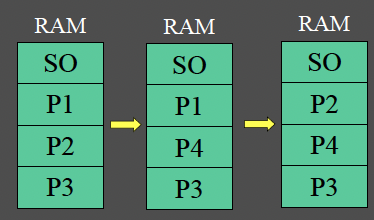
\includegraphics[width=0.5\linewidth]{images/table_swap.png}
\end{figure}
 
\begin{figure}[h]
    \centering
    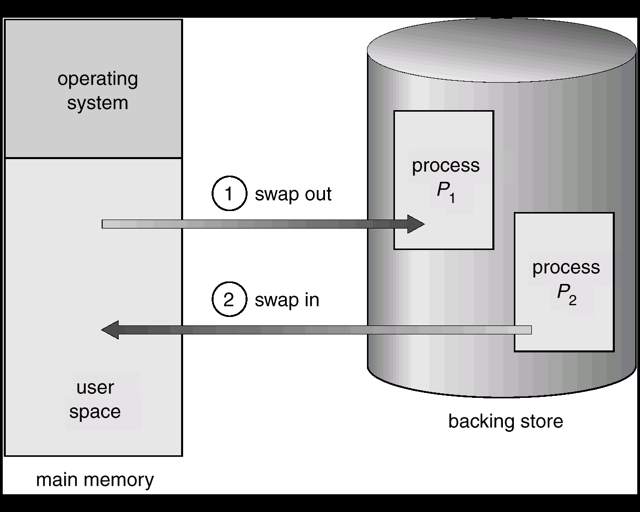
\includegraphics[width=0.5\linewidth]{images/swap-mem.png}
    \caption{Swap mem}
    \label{fig:swap-mem}
\end{figure}
Perché un programma possa essere \textbf{eseguito}, il suo codice deve trovarsi in \textbf{memoria} \textbf{primaria} (ma rivedremo questa affermazione quando parleremo della memoria virtuale)
Quindi, quando il SO riceve il \textbf{comando} di esecuzione di un programma, deve recuperare il codice del programma dalla memoria secondaria, e decidere in quale porzione della memoria primaria sistemarlo. ossia, a partire da quale indirizzo di RAM.

\section{Binding (associazione degli indirizzi)}
Un programma sorgente usa (tra l'altro) dati (variabili) e
istruzioni di controllo del flusso di computazione.
\begin{itemize}
    \item Quando il programma viene compilato e caricato in
    Memoria Primaria (MP) per essere eseguito, ad ogni
    variabile è associato l'\textbf{indirizzo} di una locazione di
    memoria che ne contiene il valore.
    \item Alle istruzioni di controllo del flusso di esecuzione del
    programma (ossia i salti condizionati e incondizionati) è
    associato l'indirizzo di destinazione del salto.
    \item L'operazione di associazione di variabili e istruzioni agli
    indirizzi di memoria è detta \textit{binding degli indirizzi}.
\end{itemize}

In altre parole, ad ogni variabile dichiarata nel programma viene fatto corrispondere l'indirizzo di una cella di memoria di RAM in cui verrà memorizzato il valore di quella variabile.
\begin{itemize}
    \item L'accesso alla variabile, in lettura e scrittura, corrisponde
    alla lettura e scrittura della cella di memoria il cui indirizzo
    è stato "legato" (con l'operazione di binding) alla variabile.
    \item Le istruzioni di salto, che permettono di implementare
    costrutti come \textit{if-then-else}, \textit{while}, ecc., sono associate agli
    indirizzi in RAM dove si trova l'istruzione con cui prosegue
    l'esecuzione del programma se il salto viene eseguito.
\end{itemize}

Ad esempio, un'istruzione C come:
\begin{verbatim}
counter = counter + 1;
\end{verbatim}
alla fine diventerà qualcosa del tipo:
\begin{verbatim}
load(R1, 10456)
Add(R1, #1);
store(R1, 10456)
\end{verbatim}
10456 è l'indirizzo della cella di memoria che contiene il
valore della variabile \textit{counter}. L'indirizzo 10456 è stato
associato alla variabile \textit{counter} durante la fase di binding
degli indirizzi.


Analogamente, un'istruzione C come:
\begin{verbatim}
while (counter <= 100) counter++;
\end{verbatim}
alla fine diventerà qualcosa del tipo:
\begin{verbatim}
100FC jgt(R1, #100, 10110) // jump if greater than
10100 load(R1, 10456)
10104 Add(R1, #1)
10108 store(R1, 10456)
1010C jmp(100FC)
10110 ... ...
\end{verbatim}

Rispetto all'indirizzo di istruzione del salto stesso, il \textit{while} della slide precedente potrebbe anche essere tradotto in assembler così:
\begin{verbatim}
100FC jgt(R1, #100, 00014) // jump if greater than
10100 load(R1, 10456)
10104 Add(R1, #1)
10108 store(R1, 10456)
1010C jmp(100FC)
10110 ... ...
\end{verbatim}

Perché un programma sorgente
possa essere eseguito deve passare
attraverso varie fasi. Il binding degli indirizzi avviene
in una di queste fasi:
\begin{itemize}
    \item compilazione
    \item caricamento (in RAM)
    \item esecuzione
\end{itemize}

\begin{figure}[h]
    \centering
    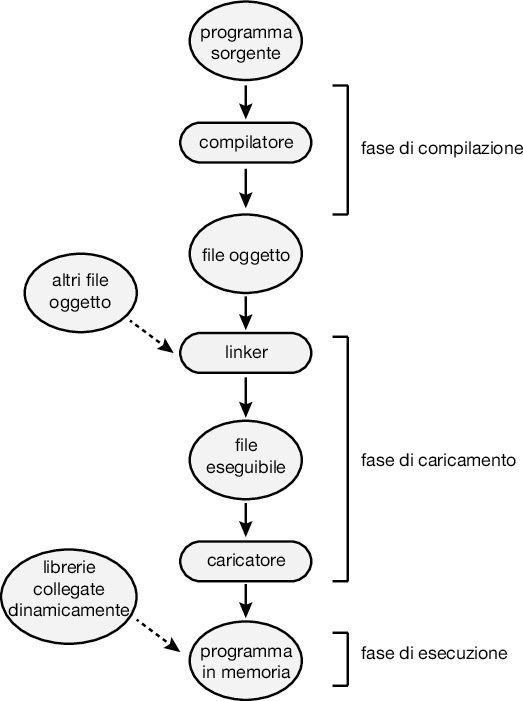
\includegraphics[width=0.25\linewidth]{images/process_compilation.png}
    \caption{Processo di compilazione da programma sorgente}
    \label{fig:compilate-process}
\end{figure}

\subsection{Quando?}
\begin{enumerate}
    \item In fase di Compilazione 
        \begin{itemize}
        \item viene generato codice assoluto o statico.
        \item Il compilatore deve conoscere l'indirizzo della cella di
        RAM a partire dal quale verrà caricato il programma,
        in modo da effettuare il \textit{binding} degli indirizzi
        (che avviene, appunto, in fase di compilazione).
        \item Se il SO deve scaricare temporaneamente il processo
        che usa quel codice in Memoria Secondaria (MS), come
        nell'esempio visto a inizio capitolo, quando lo ricarica
        in RAM deve rimetterlo esattamente dove si trovava
        prima. (Oppure?)
        \end{itemize}
    \item  In fase di caricamento in RAM
        \begin{itemize}
        \item Viene generato codice staticamente rilocabile.
        \item Il compilatore associa ad istruzioni e variabili degli
        indirizzi relativi rispetto all'inizio del programma,
        che inizia da un ipotetico indirizzo 0 virtuale.
        \item Gli indirizzi assoluti finali vengono generati in fase di
        caricamento del codice in Memoria Primaria (MP) in base all'indirizzo di
        MP a partire dal quale è caricato il codice.
        \item Il binding degli indirizzi, quindi, avviene in fase di
        caricamento del programma in RAM: se il processo che
        usa quel codice viene tolto dalla RAM, si può caricarlo
        in una posizione diversa solo rieffettuando la fase di
        caricamento (ma è più efficiente che ricompilare tutto).
        \end{itemize}
    \item In fase di esecuzione
        \begin{itemize}
        \item Viene generato codice dinamicamente rilocabile.
            \item Il codice in esecuzione usa sempre e solo indirizzi
            relativi.
            \item La trasformazione di un indirizzo relativo in uno
            assoluto viene fatta nell'istante in cui viene eseguita
            l'istruzione che usa quell'indirizzo.
            \item È necessario un opportuno supporto hardware per realizzare
            questo metodo senza perdita di efficienza.
            \item Si parla di \textit{binding dinamico} degli indirizzi.
            \item In opportuno registro di rilocazione viene usato per trasformare un indirizzo relativo nel corrispondente indirizzo assoluto durante l’esecuzione delle istruzioni.
            \item Il registro di rilocazione contiene l’indirizzo di partenza dell’area di RAM in cui è caricato il programma in esecuzione.
            \item La memory management Unit (MMU) si occuperà di trasformare gli indirizzi relativi in assoluti, usando il registro di rilocazione, per accedere alle celle di RAM indirizzate dalle istruzioni
            \item Lo spostamento del processo da un area all’altra della MP è realizzabile senza problema.
            \item Il SO deve solo ricordarsi dell’indirizzo della locazione di MP a partire dalla quale è memorizzato il processo
        \end{itemize}
        \nt{Per spostare i programmi da un’area di RAM ad un’altra ora basta cambiare l’indirizzo scritto nel registro di rilocazione (fig. 9.5 modificata)}
\end{enumerate}

\section{Spazio degli indirizzi (Logici e Fisici)}
Consideriamo codice dinamicamente rilocabile (d’ora in poi faremo sempre riferimento a codice dinamicamente rilocabile, se non indicato diversamente). Ogni indirizzo usato nel codice è riferito ad un ipotetico indirizzo 0 (zero): l’indirizzo della prima istruzione di cui è formato il codice.

Gli indirizzi utilizzati in un programma possono essere:
\begin{itemize}
    \item l'indirizzo di una cella di memoria che contiene una variabile
    \item l'indirizzo di un'istruzione di salto
\end{itemize}

Questi indirizzi rientrano nello \textbf{spazio di indirizzamento logico o virtuale}, che va da 0 all'ultima cella di memoria occupata. Quando il codice viene caricato in RAM, gli \textbf{indirizzi logici} generati dalla CPU vengono trasformati in \textbf{indirizzi fisici} attraverso il registro di rilocazione, permettendo di indirizzare correttamente la memoria fisica (RAM).

Lo \textbf{spazio di indirizzamento fisico} è l'insieme degli indirizzi fisici che dipende dall'area di memoria dove il sistema operativo ha caricato il programma.

Per i programmi con codice rilocabile dinamicamente esistono due tipi di indirizzi:
\begin{itemize}
    \item Indirizzi logici, che vanno da $0$ a $max$
    \item Indirizzi fisici, che vanno da $r+0$ a $r+max$, dove $r$ è l'indirizzo iniziale della RAM in cui il programma è caricato
\end{itemize}

Gli indirizzi logici vengono sempre mappati in indirizzi fisici per accedere correttamente alla RAM.

Le espressioni \textbf{spazio di indirizzamento logico} e \textbf{spazio di indirizzamento fisico} si riferiscono principalmente all'architettura di un sistema, non a singoli programmi.

Consideriamo un computer con un massimo di 64 Kbyte di RAM, ovvero 65536 byte. In questo contesto, possiamo dire che:
\begin{enumerate}
    \item Il computer può indirizzare $2^{16}$ byte di RAM.
    \item Gli indirizzi dei byte della RAM vanno da 0000 a FFFF in esadecimale (da 0 a $2^{16} - 1$).
    \item L'indirizzo di ciascun byte della RAM è rappresentato da 16 bit.
\end{enumerate}

Pertanto, lo \textbf{spazio di indirizzamento fisico} di questo computer è scritto su 16 bit e va da 0000 a FFFF, con una dimensione di 64 Kbyte.

Se un compilatore genera codice dinamicamente rilocabile e utilizza 12 bit (\textbf{perchè 12?}) per scrivere un indirizzo logico, lo \textbf{spazio di indirizzamento logico} di un programma sarà di massimo $2^{12}$ byte, ovvero 4 Kbyte. Nessun programma potrà superare questo limite, anche se può usare uno spazio logico inferiore.

Quindi, possiamo dire che lo spazio di indirizzamento logico dei programmi di questo computer è scritto su 12 bit, va da 0000 a 0FFF (esadecimale) ed è di 4 Kbyte.

In seguito, quando parleremo di spazi di indirizzamento, ci riferiremo a quelli dell'intera macchina, e non a quelli dei singoli programmi. Tuttavia, è possibile considerare un programma che occupa tutto lo spazio di indirizzamento logico della macchina.

\qs{}{Ha senso che la dimensione dello spazio di indirizzamento fisico sia diversa da quella dello spazio di indirizzamento logico in un sistema reale?}

In effetti, è comune che lo \textbf{spazio di indirizzamento fisico} e lo \textbf{spazio di indirizzamento virtuale} siano diversi. Nei processori moderni a 64 bit, lo spazio di indirizzamento fisico può variare da $2^{40}$ a $2^{64}$ byte (da 40 a 64 bit per gli indirizzi fisici). Tuttavia, non si usano sempre 64 bit per gli indirizzi fisici perché sono eccessivi, e un computer raramente ha una quantità di RAM pari al massimo indirizzabile dal processore (ad esempio, $2^{40}$ byte = 1 Terabyte = 1000 Gigabyte).

Sistemi operativi e applicazioni adottano spazi di indirizzamento virtuali che variano tipicamente da $2^{48}$ a $2^{64}$ byte, ovvero da 48 a 64 bit per gli indirizzi virtuali.

In generale, per i computer moderni vale la relazione:
\[
|\text{RAM}| \neq |\text{spazio di indirizzamento fisico}| \neq |\text{spazio di indirizzamento virtuale}|
\]
E di solito:
\[
|\text{RAM}| < |\text{spazio di indirizzamento fisico}| < |\text{spazio di indirizzamento virtuale}|
\]

In molti casi, per vincoli architetturali e dimensionali, la quantità effettiva di RAM di un computer è molto inferiore allo spazio di indirizzamento fisico. Pertanto, è spesso vero che:
\[
|\text{RAM}|_{\text{effettiva}} \leq |\text{RAM}|_{\text{massima}} \ll |\text{spazio fisico}| < |\text{spazio virtuale}|
\]
\clm{}{}{
Ad esempio, nei processori Intel Core i7 lo spazio di indirizzamento fisico è scritto su 52 bit, mentre quello virtuale è su 48 bit, quindi può capitare che:
\[
|\text{spazio fisico}| > |\text{spazio virtuale}|
\]
}

\qs{}{
Se un sistema ha uno spazio di indirizzamento virtuale di $X$ byte, significa che possiamo scrivere un programma che occupa al massimo $X$ byte, cioè usa indirizzi virtuali da 0 a $X-1$. Tuttavia, un programma può girare su una macchina in cui:
\[
|\text{RAM}| < |\text{spazio fisico}| < X?
\]
}

Questo aspetto sarà approfondito nel capitolo sulla \textbf{memoria virtuale}.


\section{Le librerie}
\dfn{}{
Una \textbf{libreria} è una collezione di subroutine di uso comune messe a disposizione dei programmatori per lo sviluppo software. Ad esempio, la libreria matematica del C fornisce funzioni come \texttt{sqrt(x)} per calcolare la radice quadrata.}

Le librerie sono utili perché permettono di riutilizzare codice già esistente, evitando ai programmatori di doverlo riscrivere ogni volta. Sebbene "libreria" sia una traduzione impropria di "library", il termine è ormai comunemente accettato.

\subsection{Tipi di Librerie}

Esistono principalmente due tipi di librerie:

\begin{enumerate}
    \item \textbf{Librerie statiche}: le subroutine sono collegate al programma principale durante la fase di compilazione o di caricamento, diventando parte dell'eseguibile. Tuttavia, ciò può portare a duplicazione di codice, sia su disco che in RAM, soprattutto se più programmi usano la stessa libreria. Inoltre, il codice di una libreria statica viene caricato in RAM anche se non viene utilizzato durante l'esecuzione del programma.

    \item \textbf{Librerie dinamiche}: vengono caricate in RAM solo al momento in cui il programma chiama una subroutine specifica, ossia a \textbf{run-time}. Il programma specifica solo il nome della subroutine, e il sistema operativo carica la libreria nello spazio di memoria assegnato al processo. Queste librerie sono anche dette \textbf{librerie condivise}, perché possono essere utilizzate da più processi contemporaneamente, evitando la duplicazione di codice in RAM. Inoltre, le versioni aggiornate delle librerie dinamiche possono sostituire le vecchie senza dover ricompilare i programmi che le utilizzano.
\end{enumerate}

\subsection{Estensioni delle Librerie Dinamiche}

In Unix, Linux e Solaris, le librerie dinamiche hanno estensione \texttt{.so} (shared object) e si trovano solitamente nella directory \texttt{/lib}. In ambiente Windows, le librerie dinamiche hanno estensione \texttt{.DLL} (Dynamic Link Library) e si trovano nella cartella \texttt{C:\textbackslash WINDOWS\textbackslash system32}.

\section{Tecniche di gestione della memoria primaria}
Le principali tecniche di gestione della \textbf{Memoria Principale (MP)} vanno dalle più semplici alle più complesse. Alcune di queste tecniche sono ormai obsolete, ma aiutano a comprendere concetti più avanzati. Le tecniche includono:

\begin{itemize}
    \item \textbf{Swapping}
    \item \textbf{Allocazione contigua a partizioni multiple fisse}
    \item \textbf{Allocazione contigua a partizioni multiple variabili}
    \item \textbf{Paginazione}
    \item \textbf{Paginazione a più livelli}
\end{itemize}

\subsection*{Swapping}

\dfn{}{Lo \textbf{swapping} consiste nel salvare in memoria secondaria (hard disk) l'immagine di un processo non in esecuzione (\textit{swap out}) e ricaricarla in MP (\textit{swap in}) prima di assegnarle la CPU.}

Questa tecnica permette di attivare più processi di quanti la sola MP possa contenere, utilizzando un'area dell'hard disk chiamata \textbf{area di swap}, riservata al sistema operativo. Tuttavia, se il processo viene ricaricato in una diversa area di MP, è necessario utilizzare codice dinamicamente rilocabile.

\subsubsection*{Problemi dello Swapping}

Il principale problema dello swapping è il tempo impiegato per copiare il codice e i dati di un processo tra l'hard disk e la RAM, che è nell'ordine dei millisecondi. Poiché in un millisecondo un singolo core di una moderna CPU può eseguire milioni di istruzioni, l'overhead di tempo risultante dallo swapping è generalmente considerato inaccettabile.

Di conseguenza, lo \textbf{swapping di interi processi} è ormai caduto in disuso nei moderni sistemi operativi, salvo rare eccezioni.

\subsubsection*{L'Idea di Fondo dello Swapping}

Nonostante l'obsolescenza dello swapping, l'idea di fondo rimane valida: utilizzare parte della memoria secondaria per estendere la memoria primaria, permettendo l'esecuzione di un numero maggiore di processi rispetto a quanto potrebbe ospitare la sola RAM. Questa idea sarà ripresa nel capitolo sulla \textbf{memoria virtuale}.


\section{Allocazione contigua della Memoria Primaria}
In un computer, la \textbf{Memoria Principale (MP)} è solitamente divisa in due partizioni:
\begin{itemize}
    \item una per il \textbf{Sistema Operativo (SO)}
    \item una per i \textbf{processi utente}.
\end{itemize}

Il sistema operativo si posiziona nella stessa area di memoria puntata dal \textbf{vettore delle interruzioni}, che è spesso allocato nella parte bassa della memoria.

\subsection*{Protezione della memoria}

Nei sistemi operativi più semplici (ad esempio MS-DOS), l'area non assegnata al SO viene occupata da un solo processo. La protezione della MP consiste nella protezione delle aree di memoria del SO.

\subsubsection*{Registro Limite e Registro di Rilocazione}

Il \textbf{registro limite} è inizializzato dal SO e garantisce che ogni indirizzo logico usato dal processo utente sia inferiore al valore scritto nel registro. Poiché si utilizza codice dinamicamente rilocabile, il \textbf{registro di rilocazione} viene usato per trasformare l'indirizzo logico in indirizzo fisico.

\begin{itemize}
    \item \textbf{Registro di rilocazione}: 100.040
    \item \textbf{Registro limite}: 74.600
\end{itemize}

Gli indirizzi fisici validi vanno da 100.040 a 174.640 (vedi Fig. \ref{fig:9.6}).
\begin{figure}[h]
    \centering
    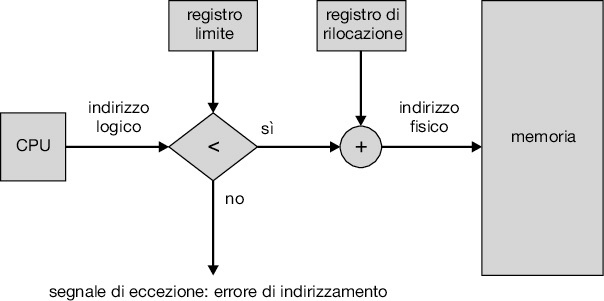
\includegraphics[width=0.5\linewidth]{images/protez_meme.png}
    \caption{Protezione memoria}
    \label{fig:9.6}
\end{figure}

\subsection{Allocazione a partizioni multiple fisse}
Nell'allocazione a partizioni fisse:
\begin{itemize}
    \item La memoria è divisa in \textbf{partizioni di dimensione fissa}, che non devono necessariamente essere tutte uguali.
    \item Ogni partizione contiene un \textbf{unico processo} dall'inizio alla fine della sua esecuzione.
    \item Il \textbf{grado di multiprogrammazione} è determinato dal numero di partizioni.
    \item Quando un processo termina, la partizione può essere occupata da un altro processo.
\end{itemize}

Il meccanismo di \textbf{registri limite e di rilocazione} protegge le partizioni da accessi non autorizzati. Durante il \textit{context switch}, il \textbf{dispatcher} carica:
\begin{itemize}
    \item Nel registro di rilocazione, l'indirizzo di partenza della partizione assegnata al processo.
    \item Nel registro limite, la dimensione della partizione.
\end{itemize}

Questa tecnica, utilizzata nel \textbf{IBM OS/360}, richiede CPU dotate di registri di rilocazione e limite, ma non è più utilizzata nei sistemi operativi moderni per i seguenti svantaggi:
\begin{itemize}
    \item Il grado di multiprogrammazione è limitato dal numero di partizioni disponibili.
    \item Si verifica \textbf{frammentazione interna}, dove una parte della partizione rimane inutilizzata se il processo è più piccolo della partizione stessa.
    \item Si può verificare \textbf{frammentazione esterna}, quando lo spazio libero disponibile è frammentato in più aree non contigue e quindi non utilizzabile per un nuovo processo di dimensione maggiore.
    \item L'arrivo di un processo più grande della partizione più grande non può essere gestito.
\end{itemize}

\textbf{Frammentazione interna}:
\begin{itemize}
    \item Parte dello spazio di memoria di una partizione viene sprecato se il processo è più piccolo della partizione stessa.
\end{itemize}

\textbf{Frammentazione esterna}:
\begin{itemize}
    \item Se la memoria libera è frammentata in più blocchi non contigui, pur avendo spazio sufficiente in totale, non può essere utilizzata per allocare nuovi processi.
\end{itemize}

L’allocazione a partizioni fisse ha anche altri problemi:
\qs{}{Che succede se arriva un processo più grande della partizione più grande?}
\clm{}{}{Notate che se si aumenta la dimensione media delle partizioni, aumenta anche la frammentazione interna, e diminuisce il grado di multiprogrammazione}

\section{Allocazione a partizioni multipli variabili}
Nell'allocazione a partizioni variabili:
\begin{itemize}
    \item Ogni processo riceve una quantità di memoria esattamente pari alla sua dimensione.
    \item Quando un processo termina, lascia un "buco" in RAM che può essere occupato da un altro processo.
    \item Tuttavia, nel tempo si creano \textbf{buchi sparsi e più piccoli}, rendendo difficile l'allocazione di nuovi processi.
\end{itemize}

\begin{figure}[h]
    \centering
    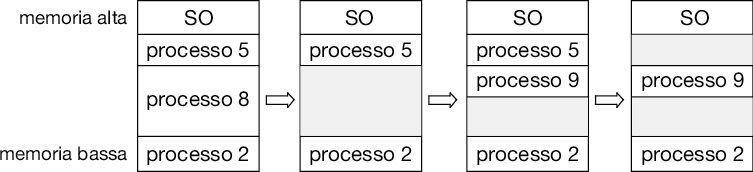
\includegraphics[width=0.5\linewidth]{images/ram_buchi.png}
    \caption{Buchi Ram}
    \label{fig:ram_hole}
\end{figure}
Il sistema operativo (SO) deve:
\begin{itemize}
    \item Tenere traccia delle aree di memoria libere e occupate.
    \item Aggiornare continuamente le informazioni quando un processo nasce o termina.
    \item Assegnare una partizione sufficientemente grande quando un nuovo processo deve essere caricato.
\end{itemize}

\subsection*{Strategie di Allocazione}
Esistono diverse strategie per scegliere quale partizione assegnare a un processo:
\begin{itemize}
    \item \textbf{First Fit}: seleziona la prima partizione abbastanza grande da ospitare il processo.
    \item \textbf{Best Fit}: seleziona la partizione più piccola che può contenere il processo.
    \item \textbf{Worst Fit}: seleziona la partizione più grande disponibile.
\end{itemize}

\textbf{Osservazioni sperimentali}:
\begin{itemize}
    \item La strategia \textbf{Worst Fit} tende a funzionare peggio in termini di utilizzo della memoria, poiché lascia spazi grandi frammentati.
    \item Le strategie \textbf{Best Fit} e \textbf{First Fit} hanno prestazioni simili, ma si preferisce \textbf{First Fit} poiché è più veloce, dato che interrompe la ricerca al primo spazio sufficiente.
\end{itemize}

\subsection{La frammentazione}
Nel tempo, l'allocazione a partizioni variabili può portare alla formazione di piccoli \textbf{buchi non contigui} in RAM:
\begin{itemize}
    \item Circa \textbf{1/3 a 1/2 della memoria principale} (MP) può essere sprecato a causa della \textbf{frammentazione esterna}, ossia la presenza di buchi di memoria troppo piccoli per ospitare un processo.
    \item Esiste anche il problema della \textbf{frammentazione interna}, dovuto all'impossibilità di tenere traccia di buchi molto piccoli che vengono quindi aggregati a partizioni adiacenti, causando uno \textbf{spreco nascosto}.
\end{itemize}

\subsubsection*{Compattazione della Memoria}

Una tecnica per recuperare la memoria inutilizzata è la \textbf{compattazione}:
\begin{itemize}
    \item Spostare le partizioni occupate dai processi in modo che siano tutte \textbf{contigue}, liberando un unico grande buco libero.
    \item La compattazione richiede la \textbf{rilocazione dinamica} del codice e dei dati dei processi.
    \item Questo processo è \textbf{costoso in termini di tempo} e durante la compattazione il sistema non è utilizzabile.
\end{itemize}

\section{Paginazione della memoria}
\dfn{}{
L’allocazione contigua della memoria principale presenta quindi diversi problemi.
L’alternativa è ammettere che l’area di memoria allocata ad un processo possa essere in realtà suddivisa in tanti pezzi non contigui fra loro
Se tutti i “pezzi” hanno la stessa dimensione allora il termine esatto per indicare questa tecnica è: paginazione della memoria (primaria)}

\subsection{Metodo di base}
La \textbf{Memoria Primaria} (o lo \textbf{spazio di indirizzamento fisico}) è suddivisa in unità dette \textbf{frame} (o pagine fisiche), con le seguenti caratteristiche:
\begin{itemize}
    \item I \textbf{frame} sono tutti della stessa dimensione, che è sempre una \textbf{potenza di due} (ad esempio: 512, 1024, 2048, fino a 8192 byte).
    \item Lo spazio di indirizzamento fisico del processo è visto come un \textbf{unico spazio contiguo} di indirizzi, ma nella realtà è suddiviso in \textbf{pagine logiche}, ciascuna di dimensione uguale ai frame fisici.
\end{itemize}

Per eseguire un processo con \textbf{x pagine}:
\begin{itemize}
    \item Il Sistema Operativo (\textbf{SO}) cerca \textbf{x frame} liberi in cui caricare le pagine del processo. Questi frame non devono essere adiacenti e le pagine possono essere caricate in un ordine qualsiasi.
    \item Ogni processo ha una propria \textbf{Tabella delle Pagine} (o \textbf{Page Table}, \textbf{PT}): un array le cui \emph{entry} contengono i numeri dei frame in cui le pagine del processo sono state caricate.
    \item Il SO tiene traccia dei \textbf{frame liberi} nella memoria primaria, utilizzandoli per memorizzare le pagine di nuovi processi.
\end{itemize}

\subsection*{Struttura della Tabella delle Pagine}
\begin{itemize}
    \item Ogni \emph{entry} della Page Table rappresenta una pagina del processo.
    \item L'indice di ciascuna entry corrisponde al numero della pagina, mentre il valore dell'entry contiene il numero del frame dove è stata memorizzata la pagina.
\end{itemize}
% \begin{figure}[h] \centering 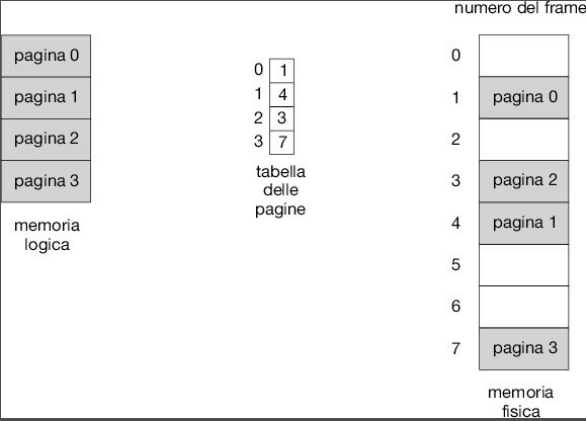
\includegraphics[width=0.50\linewidth]{images/structure_table_pagination.png} \caption{Table Pagination} \label{fig:9.9} \end{figure}
\subsection*{Problema degli Indirizzi Virtuali}
Gli \textbf{indirizzi relativi (o virtuali)} del programma, una volta caricati in RAM, non funzionano più come indirizzi lineari contigui. Ad esempio:
\begin{itemize}
    \item Un'istruzione come \texttt{jmp\_if\_odd R1,C} deve saltare a un indirizzo specifico (ad es. 0004), ma in RAM non esiste più un punto lineare di partenza.
    \item La soluzione è \textbf{riconsiderare} gli indirizzi virtuali, non più come indirizzi lineari, ma come indirizzi all'interno della Page Table, utilizzando \textbf{conversioni da indirizzi logici a indirizzi fisici}.
\end{itemize}


Indirizzi Logici e Fisici, vedere registrazione 25/10/2024 min Circa 30

\subsubsection{Paginazione: metodo di base}
Gli indirizzi logici diventano delle coppie di valori, in cui:
\begin{itemize}
    \item il primo elemento della coppia specifica il numero della pagina all’interno della quale si trova la cella di memoria che vogliamo indirizzare;
    \item il secondo elemento specifica la posizione (o offset) della cella di memoria che vogliamo indirizzare rispetto ad un ipotetico indirizzo 0 (zero), ovvero l’indirizzo del primo byte della pagina specificata dal primo elemento della coppia.
\end{itemize}
Quindi un indirizzo logico assume la forma: $(\text{pagina}, \text{offset})$.

\nt{
    Come vedremo più avanti, sotto opportune condizioni gli indirizzi logici lineari e gli indirizzi logici specificati come coppie di valori coincidono.
}

Un indirizzo logico viene tradotto in uno fisico secondo il seguente processo:
\begin{itemize}
    \item Il numero di pagina $p$ viene usato come indice nella \textit{page table} del processo per individuare il frame $f$ in cui è contenuta la pagina.
    \item Una volta noto il frame $f$ che contiene la pagina $p$, l’offset $d$ (dove "d" sta per \textit{displacement}) può essere applicato a partire dall’inizio del frame per indirizzare il byte specificato dalla coppia $(p, d)$.
\end{itemize}

Vediamo più in dettaglio: ogni informazione all’interno del computer, incluso un indirizzo logico, è in definitiva una sequenza di bit. Ad esempio: 001100010101.

Abbiamo deciso di dividere un indirizzo logico in due parti. Se abbiamo a disposizione 12 bit in tutto, dobbiamo scegliere quanti usare per specificare il numero della pagina e quanti per l’offset all’interno della pagina.

Ad esempio, possiamo decidere di utilizzare 4 bit per rappresentare il numero della pagina e i restanti 8 bit per l’offset. In questo caso, l’indirizzo logico 001100010101 rappresenta:
\begin{itemize}
    \item pagina: 3
    \item offset: 21
\end{itemize}

La scelta del numero di bit da utilizzare per scrivere il numero di pagina e l’offset dipende dall’hardware su cui dovrà girare il sistema operativo, il quale impone:
\begin{itemize}
    \item il numero di bit su cui va scritto un indirizzo logico (ad esempio $m$ bit);
    \item la dimensione di un frame, e quindi di una pagina (ad esempio $2^n$ byte).
\end{itemize}

Di conseguenza, dobbiamo utilizzare $n$ bit per rappresentare l'offset all'interno di una pagina/frame, e il numero di bit usati per rappresentare il numero di pagina sarà pari a $m - n$ bit.

\nt{
    A questo punto, la dimensione dello spazio di indirizzamento logico è stabilita come $2^{(m-n)} \times 2^n$ byte.
}

\ex{Esempio di Spazio di Indirizzamento Logico}{
    Consideriamo una macchina in cui i frame hanno dimensione $2^{12}$ byte, ovvero 4096 byte. Di conseguenza, anche la dimensione di una pagina nello spazio di indirizzamento logico del sistema sarà di 4096 byte (quindi $n = 12$).
    
    Se la macchina mette a disposizione $m = 22$ bit per rappresentare un indirizzo logico, allora il numero di bit necessari per il numero di pagina sarà $m - n = 10$ bit.
    
    In questo caso, lo spazio di indirizzamento logico della macchina risulterà pari a:
    \[
    (2^{10} \text{ pagine}) \times (2^{12} \text{ byte}) = 4 \text{ megabyte}
    \]
}

\begin{center}
    \textbf{Struttura di un Indirizzo Logico}
\end{center}
\begin{itemize}
    \item \textbf{Numero di Pagina (p)}: $m - n$ bit
    \item \textbf{Offset di Pagina (d)}: $n$ bit
\end{itemize}

\nt{
    Qui possiamo osservare uno dei tanti casi di interazione tra il sistema operativo e l’hardware sottostante. È infatti l’hardware a decidere la dimensione dei frame e il numero di bit su cui rappresentare un indirizzo logico. Il sistema operativo, quindi, deve adeguarsi a queste impostazioni.
    
    Questa configurazione consente una traduzione efficiente degli indirizzi logici in indirizzi fisici direttamente a livello hardware. Alcune parti di un sistema operativo sono infatti progettate in base allo specifico hardware su cui girerà il sistema, al fine di sfruttare al meglio le caratteristiche hardware e minimizzare l’overhead introdotto.
}

\clm{Scelta della Dimensione dei Frame}{}{
    Nei processori moderni, è possibile scegliere tra vari valori per la dimensione dei frame, e questa scelta, una volta effettuata, rimane fissa. Ad esempio:
    \begin{itemize}
        \item I processori ARM, utilizzati negli iPhone e negli iPad, permettono di scegliere tra 4KB, 16KB, 64KB, 1MB e 16MB come dimensione di un frame.
        \item La famiglia dei processori Intel, dal Pentium fino ai Core i9, consente di scegliere tra 4KB e 4MB.
        \item Gli Intel Itanium-2 offrono una gamma più ampia, con opzioni tra 4KB, 8KB, 64KB, 256KB, 1MB, 4MB, 16MB e 256MB.
    \end{itemize}
}

\dfn{Traduzione degli Indirizzi Logici in Indirizzi Fisici}{
    Definiamo più precisamente l'operazione di traduzione da indirizzi logici a indirizzi fisici. Un indirizzo logico è formato da due componenti $(p, d)$:
    \begin{itemize}
        \item \textbf{Numero di Pagina (p)}: utilizzato come indice per selezionare la entry corrispondente nella \textit{Page Table}, che contiene il numero del frame in cui è caricata la pagina.
        \item \textbf{Offset di Pagina (d)}: utilizzato all’interno del frame individuato al passo precedente per localizzare il byte specificato dall’indirizzo logico.
    \end{itemize}
}

\subsubsection{Paginazione: traduzione degli indirizzi}
Possiamo ora riassumere e integrare quanto detto finora, osservando che:

\begin{enumerate}
    \item Gli indirizzi logici nello spazio di indirizzamento logico possono essere interpretati come valori lineari oppure come coppie $(\text{pagina}, \text{offset})$.
    \item Ciascuna entry di una tabella delle pagine può contenere il numero del frame o, alternativamente, l’indirizzo di partenza del frame. Tuttavia, per ragioni pratiche, viene scelta la prima opzione: memorizzare il numero del frame.
\end{enumerate}

\nt{
    Ecco quindi la doppia natura degli indirizzi logici, che sono contemporaneamente valori lineari e coppie $(\text{pagina}, \text{offset})$.
}

Consideriamo uno spazio di indirizzamento logico di dimensione $2^m$ byte, e assumiamo che ogni pagina abbia una dimensione pari a $2^n$ byte. Un indirizzo logico lineare scritto su $m$ bit può quindi essere scomposto in:
\begin{itemize}
    \item i bit più significativi $(m - n)$, che indicano il numero di pagina $p$;
    \item i bit meno significativi $n$, che rappresentano l’offset $d$.
\end{itemize}

\begin{center}
    \textbf{Struttura di un Indirizzo Logico}
\end{center}
\begin{itemize}
    \item \textbf{Numero di Pagina (p)}: $(m - n)$ bit
    \item \textbf{Offset di Pagina (d)}: $n$ bit
\end{itemize}

\ex{Esempio di Spazio di Indirizzamento Logico}{
    Supponiamo di avere uno spazio di indirizzamento logico di 16 byte, quindi gli indirizzi logici sono rappresentati con $m = 4$ bit, poiché $2^4 = 16$. Ogni pagina ha dimensione $2^2 = 4$ byte, con $n = 2$.

    Di conseguenza, gli indirizzi logici vanno da $0000$ a $1111$, mentre il programma che occupa questo spazio è costituito dalle istruzioni/dati etichettati come "a, b, c, d, e, f, g, h, i, l, m, n" che coprono tre pagine, dove ciascuna istruzione/dato occupa un byte.
    
    \nt{
        In questo esempio, lo spazio di indirizzamento logico del programma è suddiviso in pagine. Gli indirizzi di istruzioni e dati, che costituiscono lo spazio di indirizzamento logico, sono quindi valori consecutivi che vanno da $0000$ (prima istruzione) a $1011$ (ultima istruzione).
    }
    
    Osserviamo come gli $(m - n)$ bit più significativi di ciascun indirizzo rappresentano il numero di pagina, mentre i restanti $n$ bit meno significativi indicano l'offset all'interno della pagina.
}

\begin{center}
    \begin{tabular}{cc}
        \textbf{Indirizzo Logico} & \textbf{Contenuto} \\
        \hline
        \textbf{00 00} & a \\
        \textbf{00 01} & b \\
        \textbf{00 10} & c \\
        \textbf{00 11} & d \\
        \textbf{01 00} & e \\
        \textbf{01 01} & f \\
        \textbf{01 10} & g \\
        \textbf{01 11} & h \\
        \textbf{10 00} & i \\
        \textbf{10 01} & l \\
        \textbf{10 10} & m \\
        \textbf{10 11} & n \\
    \end{tabular}
\end{center}

Ogni indirizzo è quindi composto da:
\begin{itemize}
    \item I primi due bit, che rappresentano il numero di pagina:
    \begin{itemize}
        \item $00$ per la pagina 0
        \item $01$ per la pagina 1
        \item $10$ per la pagina 2
    \end{itemize}
    \item Gli ultimi due bit, che rappresentano l’offset all’interno della pagina.
\end{itemize}

\nt{
    Supponiamo ora di caricare il programma in RAM. Utilizziamo 5 bit per rappresentare un indirizzo fisico, quindi lo spazio di indirizzamento fisico ha dimensione pari a $2^5 = 32$ byte. Tuttavia, la nostra macchina è dotata di soli 20 byte di RAM, suddivisi in 5 frame, ciascuno con un indirizzo che va da $00000$ a $10011$.
}

\ex{Esempio di Traduzione Indirizzo Logico in Indirizzo Fisico}{
    Consideriamo l’indirizzo logico $0010$. La sua conversione in un indirizzo fisico procede così:
    \begin{enumerate}
        \item \textbf{Numero di Pagina}: il numero di pagina (0) è utilizzato per accedere alla \textit{Page Table}, che ci indica che la pagina 0 è caricata nel frame 4.
        \item \textbf{Offset}: l'offset di 2 bit $(10)$ viene applicato a partire dall’indirizzo iniziale del frame 4.
    \end{enumerate}
    Di conseguenza, l’indirizzo fisico risultante è $10010$.
}

% \begin{figure}[h] \centering 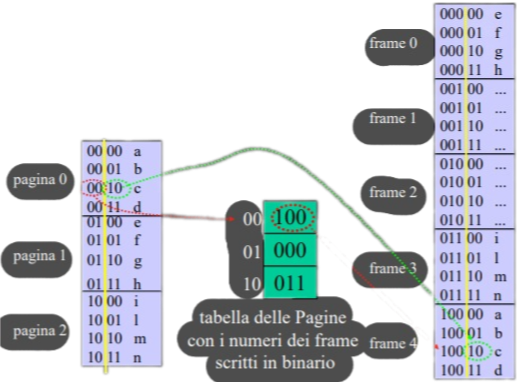
\includegraphics[width=0.25\linewidth]{images/pagination_example.png} \caption{Esempo di paginazione} \label{fig:9.10} \end{figure}

\clm{Struttura di un Indirizzo Fisico}{}{
    Notiamo un aspetto importante: nei nostri indirizzi fisici, i bit più significativi (5 - 2 = 3 bit) indicano il numero di frame corrispondente. Ad esempio, per l’indirizzo $10010$, i primi 3 bit $100$ identificano il frame 4.
}

\nt{
    Le pagine e i frame sono configurati per avere una dimensione $|P|$ pari a una potenza di 2, ossia $|P| = 2^n$. Grazie a questa proprietà, l'offset all'interno di ogni pagina o frame varia da una configurazione di tutti zeri a una di tutti uno:
    \[
        \text{Offset valido: } 00 \dots 00 \text{ a } 11 \dots 11.
    \]
    Di conseguenza, l’indirizzo di partenza di ogni pagina o frame richiede che gli $n$ bit meno significativi siano impostati a 0.
}

\clm{Struttura degli Indirizzi di Partenza}{}{
    Gli indirizzi logici di inizio pagina nello spazio di indirizzamento di un programma avranno la forma seguente:
    \[
        \begin{array}{l}
            00 \dots 00 \; 00 \dots 00 \quad \text{inizio della pagina 0} \\
            00 \dots 01 \; 00 \dots 00 \quad \text{inizio della pagina 1} \\
            00 \dots 10 \; 00 \dots 00 \quad \text{inizio della pagina 2} \\
            00 \dots 11 \; 00 \dots 00 \quad \text{inizio della pagina 3}
        \end{array}
    \]
    Lo stesso vale per i frame nello spazio di indirizzamento fisico.
}

\nt{
    Se rimuoviamo gli $n$ bit meno significativi da un indirizzo logico di $m$ bit, i rimanenti $m - n$ bit contano semplicemente le pagine (in binario) in cui è suddiviso lo spazio di indirizzamento logico. Ad esempio:
    \[
        \begin{array}{l}
            00 \dots 00 = \text{pagina 0} \\
            00 \dots 01 = \text{pagina 1} \\
            00 \dots 10 = \text{pagina 2} \\
            00 \dots 11 = \text{pagina 3}
        \end{array}
    \]
    Questa logica vale anche per i frame nello spazio fisico, utilizzando un numero di bit adeguato per rappresentare i frame.
}

\ex{Ricostruzione dell'Indirizzo Fisico}{
    Supponiamo di avere un indirizzo logico in cui il numero di pagina e l’offset sono rappresentati come segue:
    \[
        \text{Numero di pagina } = 001010, \quad \text{Frame } = 1110001
    \]
    \[
        \text{Offset } = 101010
    \]
    Allora, l’indirizzo logico diventa $001010101010$, mentre l’indirizzo fisico corrispondente sarà $1110001101010$.
}

\nt{
    La conversione da indirizzo logico a fisico si basa sull’operazione di somma dell'indirizzo base del frame con l'offset, ad esempio:
    \[
        \begin{array}{l}
            \text{Indirizzo base del frame: } 1110001000000 \\
            \text{Offset: } \phantom{\text{Indirizzo base del frame: }} 101010
        \end{array}
    \]
    Somma:
    \[
        1110001000000 + 101010 = 1110001101010
    \]
}

\clm{Efficienza della Traduzione}{}{
    Se le dimensioni di pagine e frame sono potenze di due:
    \begin{enumerate}
        \item Non è necessario effettuare la somma tra l'indirizzo base del frame e l'offset, risparmiando tempo di calcolo.
        \item Non è necessario memorizzare l'indirizzo di base in ogni entry della page table, ma solo il numero del frame, poiché gli $n$ bit meno significativi dell'indirizzo di partenza sono tutti a 0, con un risparmio di spazio.
    \end{enumerate}
    Generare un indirizzo fisico diventa quindi un’operazione di concatenazione veloce tra il numero di frame e l'offset, eseguibile direttamente dall’hardware.
}

\nt{
    Quando le dimensioni di pagine e frame sono potenze di due, possiamo interpretare l’operazione di calcolo dell'indirizzo fisico come una concatenazione, anziché una somma:
    \[
        1110001000000 + 101010 = 1110001101010 \quad \Rightarrow \quad 1110001 \text{ “attaccato a” } 101010.
    \]
    Usando potenze di due, la costruzione dell'indirizzo fisico è più semplice e può essere gestita velocemente dall’hardware.
}

\ex{Esempio: Dimensione della Page Table}{
    Consideriamo un sistema in cui:
    \begin{itemize}
        \item l’indirizzo fisico è su 38 bit,
        \item l’indirizzo logico è su 40 bit,
        \item una pagina è di 8 Kbyte, quindi $2^{13}$ byte.
    \end{itemize}
    
    La dimensione della page table più grande possibile per questo sistema si calcola come segue:
    
    \begin{enumerate}
        \item \textbf{Calcolo del numero di entry nella page table}:
        \[
            \frac{2^{40} \text{ byte}}{2^{13} \text{ byte}} = 2^{27} \text{ entry}.
        \]
        
        \item \textbf{Numero di bit necessari per ogni entry}: Ogni entry deve essere in grado di indirizzare un frame nello spazio fisico. Lo spazio di indirizzamento fisico è diviso in:
        \[
            \frac{2^{38} \text{ byte}}{2^{13} \text{ byte}} = 2^{25} \text{ frame}.
        \]
        Il numero minimo di byte per rappresentare un frame è di 4 byte.
        
        \item \textbf{Calcolo della dimensione totale della page table}:
        \[
            2^{27} \times 2^2 \text{ byte} = 2^{29} \text{ byte} = 512 \text{ Mbyte}.
        \]
    \end{enumerate}
}
La paginazione permette di separare lo spazio di indirizzamento logico da quello fisico. Ogni programma “vede” la memoria come uno spazio contiguo che parte sempre dall'indirizzo logico 0, ma in realtà il programma è distribuito in diversi frame fisici, sparsi in memoria assieme ad altri programmi.
La paginazione introduce una protezione automatica dello spazio di indirizzamento. Un processo può accedere solo ai frame elencati nella sua page table, poiché ogni page table viene gestita e costruita dal sistema operativo per ciascun processo.

\clm{Vantaggi e Limiti della Paginazione}{}{
    \begin{itemize}
        \item \textbf{Eliminazione della frammentazione esterna}: Ogni frame libero può essere utilizzato per memorizzare una pagina, riducendo gli sprechi di memoria.
        \item \textbf{Frammentazione interna}: Rimane una media di mezza pagina per processo, poiché l’ultima pagina del processo può non occupare completamente il frame assegnato.
        \item \textbf{Rilocazione dinamica}: La paginazione implementa una forma di rilocazione dinamica, dove ogni pagina è mappata su un diverso valore del registro di rilocazione, ossia l’indirizzo di partenza del frame che contiene la pagina.
    \end{itemize}
}

\subsection{Rilocazione Dinamica}

\subsubsection{Rilocazione Dinamica Tramite Registri di Limite e di Rilocazione}
La \textbf{rilocazione dinamica} viene gestita inizialmente utilizzando due registri principali:
\begin{itemize}
    \item \textbf{Registro di limite}: Controlla che l’indirizzo logico rientri nello spazio di indirizzamento del processo. Se l’indirizzo eccede questo limite, il sistema lancia un’eccezione di indirizzamento.
    \item \textbf{Registro di rilocazione}: Viene usato per traslare l’indirizzo logico approvato in un indirizzo fisico, aggiungendo il valore del registro di rilocazione all’indirizzo logico (vedi Fig. 9.6).
\end{itemize}
Questo approccio verifica dunque prima la validità dell'indirizzo logico rispetto allo spazio di indirizzamento del processo, per poi calcolare l’indirizzo fisico finale.
\subsubsection{Rilocazione Dinamica di Ogni Singola Pagina Tramite la Page Table}
Con la \textbf{paginazione}, la gestione della rilocazione dinamica cambia in quanto:
\begin{itemize}
    \item La suddivisione in pagine elimina la necessità di un controllo tramite il registro limite. 
    \item Ogni indirizzo logico è diviso in \textbf{numero di pagina} e \textbf{offset}, dove l’offset rappresenta sempre una posizione interna al frame associato, eliminando il rischio di indirizzamenti fuori dai limiti (vedi Fig. 9.8).
\end{itemize}
In questo caso, il controllo e la mappatura degli indirizzi sono effettuati dalla page table, la quale memorizza l’indirizzo di ciascun frame per ogni pagina del processo attivo.

\subsection{Dimensione delle Pagine e Gestione della Tabella delle Pagine}

\subsubsection{Dimensione Storica delle Pagine}
Nel tempo, la \textbf{dimensione delle pagine} di memoria è aumentata progressivamente per adattarsi alle esigenze di gestione della memoria dei sistemi operativi:
\begin{itemize}
    \item Le dimensioni comuni oggi includono pagine da \textbf{4 KB}, \textbf{8 KB}, \textbf{16 KB} e possono arrivare fino a \textbf{256 MB}.
    \item \textbf{Vantaggi di pagine più grandi}: Permettono di ridurre la lunghezza delle page table, il che riduce lo spazio richiesto in RAM per mantenere la tabella. 
    \item \textbf{Svantaggi di pagine più grandi}: Producono una maggiore frammentazione interna, poiché una pagina più grande può avere porzioni non completamente utilizzate da un processo.
\end{itemize}

\subsubsection*{Page Table e Frame Table}
A ogni processo è associata una \textbf{tabella delle pagine (page table)}, che contiene informazioni sui frame assegnati alle pagine del processo. La gestione della memoria fisica richiede inoltre che il sistema operativo mantenga una \textbf{frame table}, che descrive lo stato di ogni frame nella memoria fisica:
\begin{itemize}
    \item Indica quali frame sono liberi e quali sono occupati.
    \item Registra quale pagina di quale processo occupa ogni frame.
\end{itemize}

\subsubsection*{Attivazione della Page Table e Contesto del Processo}
Ogni volta che avviene un \textbf{context switch} (ovvero, quando la CPU passa da un processo a un altro), il sistema operativo deve attivare la page table del nuovo processo:
\begin{itemize}
    \item Ciò comporta un \textbf{tempo di configurazione} aggiuntivo durante il cambio di contesto, poiché la page table del nuovo processo deve essere caricata e attivata.
    \item L’attivazione della page table incide sulle performance del sistema, rallentando potenzialmente il cambio di contesto.
\end{itemize}

\subsubsection*{Supporto Hardware alla Paginazione}
La \textbf{paginazione richiede un supporto hardware} per garantire efficienza, poiché ogni accesso alla memoria passa per il meccanismo di traduzione da indirizzi logici a indirizzi fisici. La sfida principale risiede nella gestione della page table:
\begin{itemize}
    \item Ogni indirizzo logico generato dalla CPU deve passare attraverso una entry della page table, quindi l’\textbf{accesso alla page table deve essere rapido}.
    \item In sistemi con un numero ridotto di pagine per processo, come nel caso del \textbf{PDP-11} (che utilizzava \textbf{8 registri} per memorizzare la page table con una memoria fisica di 64 KB, divisa in 8 frame da 8 KB), la page table poteva essere memorizzata in registri della CPU.
    \item Tuttavia, nei computer moderni, le page table contengono migliaia di entry e non è possibile mantenerle tutte all’interno dei registri della CPU.
\end{itemize}

\subsection{Supporto Hardware}
Siamo costretti a tenere la PT di ogni processo in MP, consumando spazio. Questo rende preferibile l'uso di pagine più grandi.
Per accedere a un dato all’indirizzo logico $I$, dobbiamo prima accedere alla RAM per recuperare il numero del frame e calcolare l’indirizzo fisico, e solo successivamente utilizzarlo per leggere il dato. In questo modo il numero di accessi alla memoria principale raddoppia, il che è inaccettabile, poiché un accesso in RAM può costare oltre 100 cicli di clock, rispetto ai 5 cicli necessari se il dato si trova in un registro o nella cache L1 della CPU.
Per migliorare l'efficienza e ridurre i tempi di accesso alla PT, si utilizza una tecnica di caching della PT tramite una memoria associativa della CPU, detta \emph{Translation Look-aside Buffer} (TLB). Questo esempio mostra come i progettisti hardware possano dotare i processori di dispositivi che facilitano e ottimizzano il lavoro del SO.
Per facilitare l’accesso rapido alla PT, il sistema operativo ha anche un registro dedicato che contiene l’indirizzo di partenza della PT del processo attivo, detto \emph{Page-Table Base Register} (PTBR). Durante un \emph{context switch}, è sufficiente aggiornare il valore del PTBR per “attivare” la PT del nuovo processo in esecuzione.
La memoria associativa è costituita da coppie chiave–valore. Fornendo una chiave come input, essa viene confrontata simultaneamente con tutte le chiavi memorizzate, restituendo il valore associato. Questo dispositivo, benché molto veloce e costoso, ha dimensioni ridotte (tra 64 e 1024 elementi).
\begin{figure}[h] \centering 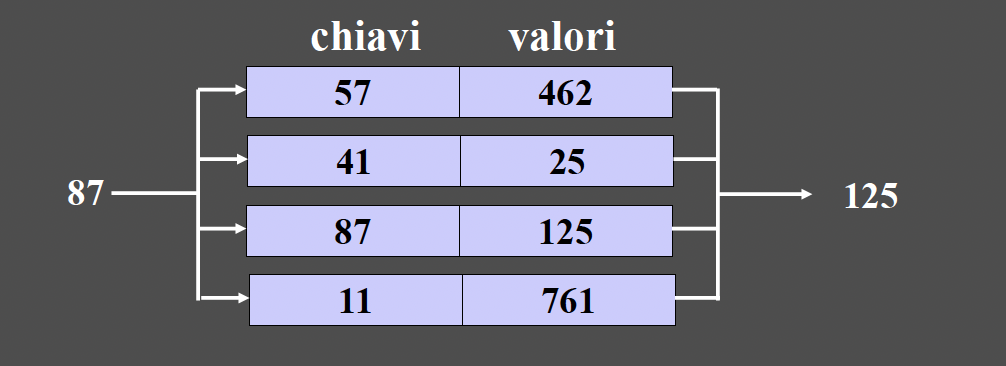
\includegraphics[width=0.50\linewidth]{images/chiave-valorePTB.png} \caption{chiave-valorePTB} \label{fig:9.9} \end{figure}

La TLB contiene una porzione della PT, costituita da coppie chiave–valore sotto forma di numero di pagina (chiave) e relativo frame (valore). Quando viene generato un indirizzo logico, il numero di pagina viene fornito alla TLB per ottenere il frame associato.

\cor{Hit Ratio nella TLB}{
    Il termine \emph{Hit Ratio} indica la percentuale di successi (hit) nella ricerca del numero di pagina nella TLB. Un maggiore hit ratio implica una minore degradazione delle prestazioni.
}

\ex{Calcolo delle prestazioni con e senza TLB}{
    Supponiamo: 1) un TLB perfetto, ossia accedere al TLB non costa tempo; 2) 10 nanosec per accedere alla RAM una volta tradotto l’indirizzo logico in fisico; 3) \emph{hit ratio} pari all'80\%. Il tempo medio di accesso in RAM sarà:
    
    \[
    10 \, \text{nsec} \times 0,80 + (10 + 10) \, \text{nsec} \times 0,20 = 12 \, \text{nsec}
    \]

    Il che comporta una degradazione delle prestazioni del 20\%.

    Se il TLB avesse invece un \emph{hit ratio} del 99\%, il tempo medio di accesso alla memoria sarebbe:

    \[
    10 \, \text{nsec} \times 0{,}99 + (10 + 10) \, \text{nsec} \times 0{,}01 = 10{,}1 \, \text{nsec}
    \]

    Questo porterebbe a una degradazione delle prestazioni di appena l'1\%.

    Se, invece, consideriamo che il TLB abbia un tempo di accesso maggiore di zero, diciamo all'incirca 1 nsec (cioè un decimo del tempo di accesso in RAM), con un \emph{hit ratio} del 99\% il tempo medio di accesso alla memoria sarebbe:

    \[
    (10 + 1) \, \text{nsec} \times 0{,}99 + (10 + 10) \, \text{nsec} \times 0{,}01 = 11{,}09 \, \text{nsec}
    \]

    In questo caso la degradazione delle prestazioni sarebbe di quasi l'11\%.

    Quando si verifica un \emph{miss} nella TLB, la coppia pagina-frame mancante viene recuperata attraverso la PT in RAM e copiata nella TLB. Questo permette che i successivi riferimenti alla stessa pagina usino la copia memorizzata nella TLB, riducendo il tempo di accesso.

    Se il TLB è pieno, una delle sue \emph{entry} deve essere sovrascritta, solitamente scegliendo l'elemento meno recentemente utilizzato (Least Recently Used, LRU) o selezionandone uno casuale.

    \nt{
    Al \emph{context switch} il TLB deve essere svuotato; verrà successivamente ripopolato con le coppie pagina-frame del nuovo processo in esecuzione.
    }

}

\subsection{Pagine condivise}
Quando due processi eseguono lo stesso codice, mantenere in memoria principale (MP) due copie identiche del codice non solo è inutile, ma spreca anche spazio in RAM. La paginazione facilita la condivisione del codice, poiché permette di memorizzare una sola copia di codice, condivisa tra i processi. Questo è possibile perché il codice, essendo \emph{non modificabile} durante l'esecuzione, viene definito come \emph{codice puro} o \emph{rientrante}.

\nt{
Una pagina condivisa può essere utilizzata per contenere codice di librerie dinamiche che diversi processi possono usare contemporaneamente, riducendo ulteriormente lo spazio richiesto in MP per il codice eseguito da più processi.
}

\begin{figure}[h] \centering 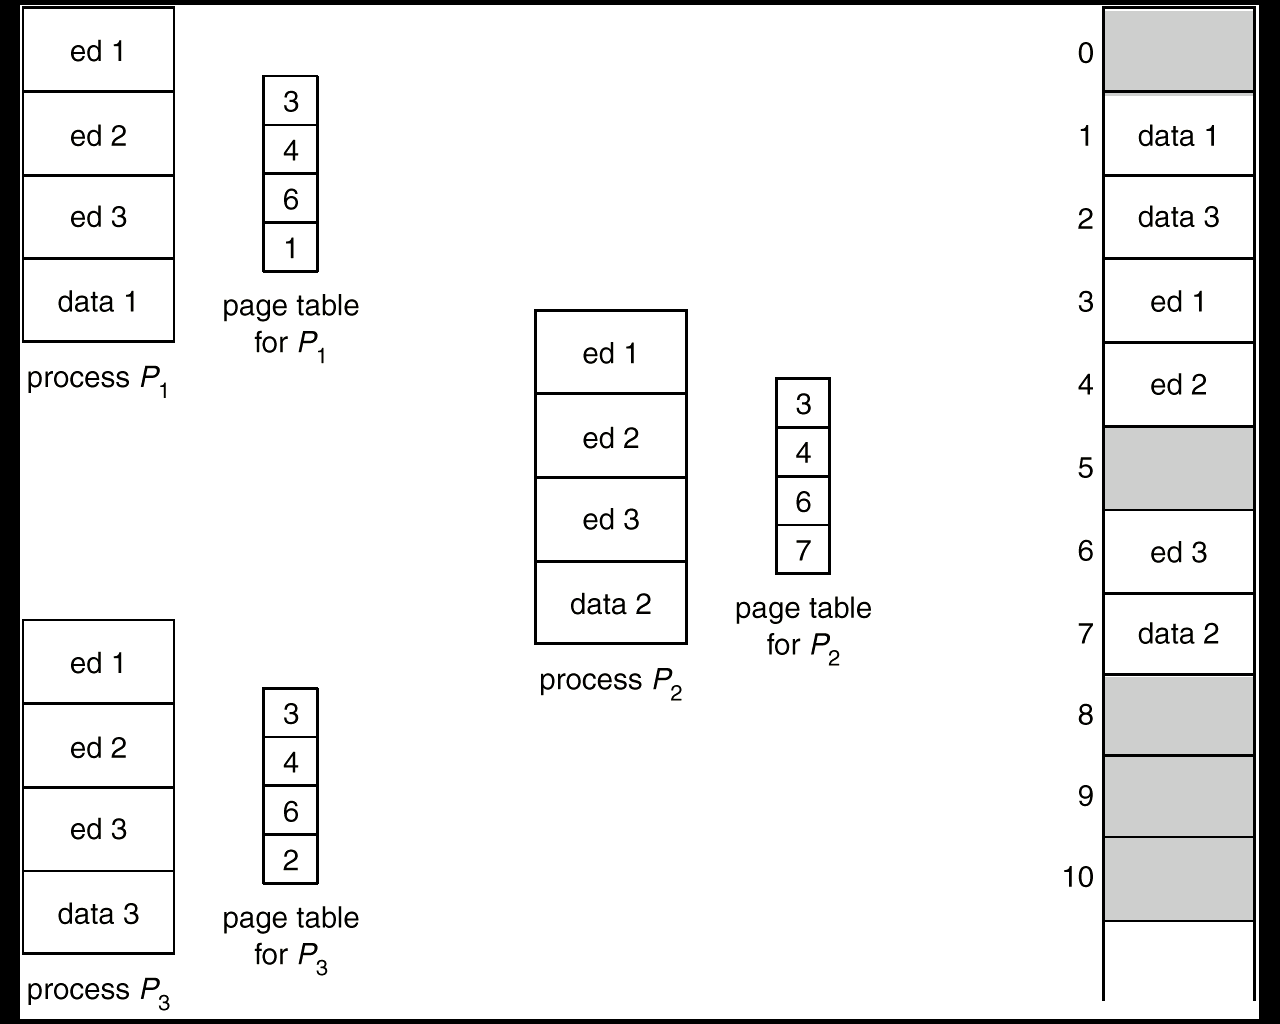
\includegraphics[width=0.45\linewidth]{images/shared_code_paginatedEnv.png} \caption{shared_code_paginatedEnv.png} \label{fig:9.9} \end{figure}

\section{Paginazione a più livelli}

Nei moderni calcolatori, lo spazio di indirizzi logici può ormai raggiungere anche \(2^{64}\) byte. Per un sistema con \(2^{32}\) byte di spazio logico e pagine da 4 Kbyte (\(2^{12}\) byte), la \emph{Page Table} (PT) può avere fino a un milione (\(2^{20}\)) di entry. Se ogni entry occupa 4 byte, la PT del processo occuperà quindi 4 Mbyte, richiedendo ben 1024 frame per essere completamente contenuta in memoria principale (MP).

\qs{} {
Considerando questi numeri, è possibile ipotizzare la dimensione massima dello spazio di indirizzamento fisico del sistema?
}

Assumendo uno spazio logico di \(2^{32}\) byte, pagine da 4 Kbyte (\(2^{12}\) byte), e una dimensione di 4 byte per ogni entry della PT, si ha che ogni entry della PT deve contenere il numero di un frame del sistema. Con 32 bit a disposizione, possiamo numerare fino a \(2^{32}\) frame (dal frame 0 al frame \(2^{32}-1\)). Dunque, lo spazio di indirizzamento fisico del sistema può contenere al massimo \(2^{32}\) frame e avere una dimensione massima di \(2^{32} \times 2^{12} = 2^{44}\) byte.

\nt{
L'uso della paginazione consente di evitare la necessità di allocare grandi aree contigue di memoria principale, ma può succedere che la PT del processo attivo sia comunque molto grande, creando problemi di allocazione.
}

Una possibile soluzione consiste nell'implementare una \emph{paginazione a due livelli}, che suddivide la PT in pagine memorizzate in frame non adiacenti in MP. In questo caso, la PT vera e propria (ora chiamata \emph{PT interna}) richiede una \emph{PT esterna}, che indica in quali frame sono memorizzate le pagine della PT interna.

\ex{Esempio di paginazione a due livelli}{
Consideriamo una macchina con 32 bit di spazio di indirizzamento logico e fisico, e con pagine/frame da 4 Kbyte. In questo caso, un indirizzo logico sarà composto da:
\begin{itemize}
    \item 20 bit per il numero della pagina 
    \item 12 bit per l'offset all'interno della pagina.
\end{itemize}

Il numero di pagina \(p\), espresso su 20 bit, sarà quindi ulteriormente suddiviso in:
\begin{itemize}
    \item 10 bit più significativi (\(p_1\)): entry della PT esterna, che punta al frame \(F_1\) contenente una porzione della PT interna.
    \item 10 bit intermedi (\(p_2\)): offset nel frame \(F_1\).
\end{itemize}

Pertanto, l'indirizzo logico sarà strutturato come segue:

\[
\text{p} = \text{p}_1 \ \text{p}_2 \ \text{d}
\]
dove:
\begin{itemize}
    \item \(p_1\): 10 bit per la pagina esterna
    \item \(p_2\): 10 bit per la pagina interna
    \item \(d\): 12 bit per l'offset all'interno della pagina.
\end{itemize}
}
\begin{figure}[h] \centering 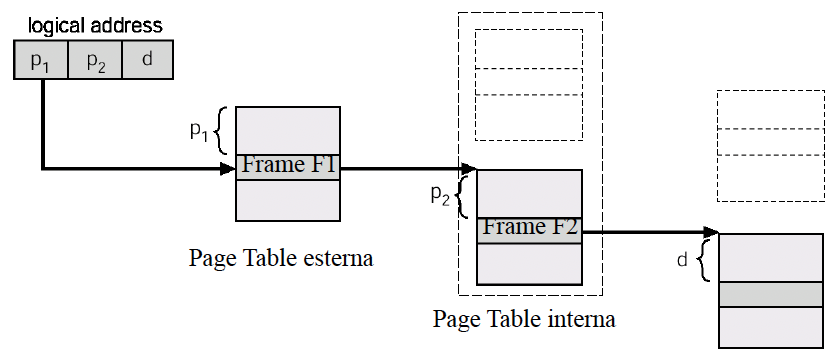
\includegraphics[width=0.50\linewidth]{images/traduzione_indirizzi_paginazione2Livelli.png} \caption{traduzione_indirizzi_paginazione2Livelli.png} \label{fig:9.16} \end{figure}

\ex{Esempio di calcolo dell'indirizzo fisico}{
Per comprendere il funzionamento della paginazione a due livelli in termini numerici, consideriamo un sistema in cui ogni entry delle PT occupa 4 byte (anche se tecnicamente sarebbero sufficienti 20 bit, poiché il numero massimo di frame è limitato). Prendiamo in esame la PT più grande, denominata \emph{PT interna}, che contiene \(2^{20}\) entry e quindi ha una dimensione di \(4 \times 2^{20}\) byte, richiedendo esattamente \(2^{10} = 1024\) frame.

La PT interna è quindi memorizzata in 1024 frame non contigui. Per tracciare la loro allocazione, il sistema operativo costruisce una \emph{PT esterna}, che occupa esattamente un frame (poiché ciascuna delle sue 1024 entry occupa 4 byte).

I passi per tradurre un indirizzo logico \(V\) di 32 bit in un indirizzo fisico sono i seguenti:
\begin{itemize}
    \item I 10 bit più significativi di \(V\), indicati come \(p_1\), servono per individuare una delle 1024 entry nella PT esterna, che funziona come un array di 1024 entry da 4 byte ciascuna.
    \item In questa entry, viene recuperato il numero del frame \(F_1\) che contiene una delle pagine della PT interna.
    \item Utilizzando i 10 bit intermedi di \(V\) (\(p_2\)), accediamo a una delle 1024 entry del frame \(F_1\). Questa entry contiene il numero del frame \(F_2\) che memorizza la pagina dell'indirizzo logico \(V\) (definito ora da \(p_1 p_2\)).
    \item Infine, aggiungendo l'offset \(d\) a \(F_2\), otteniamo l'indirizzo fisico finale.
\end{itemize}
}
\begin{figure}[h] \centering 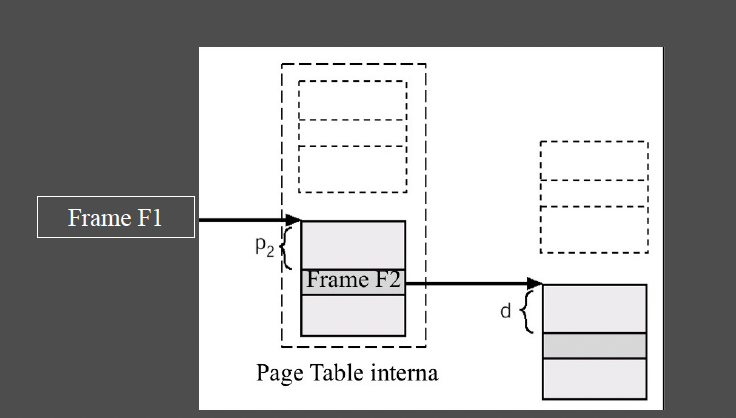
\includegraphics[width=0.50\linewidth]{images/ex_paginazione2Livelli.png} \caption{ex_paginazione2Livelli.png} \label{fig:9.17} \end{figure}


\section{Paginazione a due livelli}
La \textbf{paginazione a due livelli} è stata utilizzata, ad esempio, nei vecchi processori Pentium (lo vedremo successivamente come esempio pratico). Altre architetture, come la \textbf{VAX} di Digital Equipment Corporation (DEC), implementavano una \emph{PT esterna} composta da soli 4 elementi.

\qs{Gestione dello spazio logico su 64 bit}{
Che cosa accade con uno spazio di indirizzamento logico di 64 bit?\\
\textbf{Dimostrazione:} Con pagine da 4 Kbyte e 4 byte per entry nelle PT, la PT esterna può arrivare a occupare \(2^{44}\) byte. (Provate a verificare questo valore!)
}

Consideriamo ora la \textbf{PT interna} più grande con un indirizzamento logico a 64 bit:
\begin{itemize}
    \item Tale PT richiede \( \frac{2^{64}}{2^{12}} = 2^{52}\) entry, occupando dunque \(2^{52} \times 2^2 = 2^{54}\) byte.
    \item Questo corrisponde a \(\frac{2^{54}}{2^{12}} = 2^{42}\) frame.
    \item La PT esterna necessiterà quindi di \(2^{42}\) entry, ognuna da 4 byte, raggiungendo una dimensione di \(2^{42} \times 2^2 = 2^{44}\) byte.
\end{itemize}

\nt{
Con un indirizzamento logico a 64 bit, anche la PT esterna diventa così grande da necessitare una paginazione ulteriore. Questo problema non si limita alle architetture a 64 bit; anche alcune architetture a 32 bit implementavano paginazioni su più livelli:
}

\begin{itemize}
    \item \emph{SPARC} (SUN Microsystems) a 32 bit: utilizzava una paginazione a 3 livelli.
    \item CPU a 32 bit \emph{Motorola 68030}: implementava uno schema di paginazione a 4 livelli.
\end{itemize}

\clm{Overhead della paginazione su architetture a 64 bit}{}{
In sistemi a 64 bit, nemmeno 4 livelli di paginazione risultano sufficienti. Per esempio, l'architettura \emph{UltraSPARC} richiede fino a 7 livelli di paginazione. Se una pagina non è disponibile nel \emph{TLB}, la traduzione da indirizzo logico a fisico può richiedere l'attraversamento di 7 livelli di pagine in RAM, causando un notevole overhead.
}


\subsection{Page Table Invertita (IPT)}
Una soluzione alternativa adottata in alcune architetture a 64 bit è la \textbf{Tabella delle Pagine Invertita (IPT)}, la cui gestione presenta caratteristiche diverse rispetto alla paginazione tradizionale.

\begin{itemize}
    \item Una \emph{IPT} descrive l’occupazione dei frame nella memoria fisica. Al contrario delle \emph{PT}, esiste una sola \emph{IPT} per tutto il sistema (invece di una per ciascun processo), riducendo così lo spreco di memoria.
    \item La dimensione dell’\emph{IPT} dipende esclusivamente dalla dimensione della memoria primaria: ogni entry rappresenta un frame specifico, e il numero di entry totali equivale al numero di frame.
    \item L’indice di ogni entry dell’\emph{IPT} corrisponde al numero di un frame in memoria principale.
\end{itemize}

Ogni entry dell'\emph{IPT} è costituita da una coppia di valori:
\[
\langle \text{process-id}, \text{page-number} \rangle
\]
dove:
\begin{itemize}
    \item \emph{process-id} identifica il processo proprietario della pagina.
    \item \emph{page-number} indica il numero della pagina contenuta nel frame rappresentato da quella entry.
\end{itemize}

\begin{quote}
Ogni indirizzo logico generato dalla CPU è quindi una tripla:
\[
\langle \text{process-id}, \text{page-number}, \text{offset} \rangle
\]
Per generare l'indirizzo fisico, si cerca nella \emph{IPT} la coppia \(\langle \text{process-id}, \text{page-number} \rangle\). Se viene trovata nella \(i\)-esima entry, l'indirizzo fisico sarà \(\langle i, \text{offset} \rangle\).
\end{quote}

\clm{Vantaggi e svantaggi dell’IPT}{}{
Utilizzare una \emph{IPT} permette di risparmiare spazio, ma può aumentare il tempo di traduzione degli indirizzi logici in fisici, in quanto:
\begin{itemize}
    \item Per ottenere l’indirizzo fisico, è necessario scorrere la \emph{IPT} alla ricerca della entry contenente la coppia \(\langle \text{process-id}, \text{page-number} \rangle\), il che può richiedere centinaia o migliaia di accessi alla memoria principale (MP) se la \emph{IPT} è memorizzata in RAM.
    \item Tuttavia, l’uso di \emph{memorie associative} per contenere tutta o parte dell’\emph{IPT} consente la traduzione della maggior parte degli indirizzi senza un significativo impatto sulle prestazioni.
\end{itemize}
}

\section{Il supporto alla paginazione nei vecchi processori Intel}
La paginazione può, in teoria, essere implementata senza supporto hardware, ma un aiuto dall'hardware è fondamentale se si vogliono evitare significative degradazioni delle prestazioni. Oltre al supporto essenziale fornito dal \emph{Translation Lookaside Buffer (TLB)}, tutti i processori moderni offrono una gamma di facilitazioni per una gestione efficiente dei riferimenti in memoria.

Un esempio classico è rappresentato dalla famiglia dei vecchi processori Intel Pentium (ad esempio, Pentium 3 e 4). 

A scelta del sistema operativo che gira sul processore, è possibile utilizzare pagine da 4 Kbyte o da 4 Mbyte. Nel caso di pagine da 4 Kbyte, il processore adotta uno schema di paginazione a due livelli. La traduzione degli indirizzi da logici a fisici avviene nel modo consueto attraverso l'unità di paginazione:


\section{Conclusioni}
// TODO: :D
\afterpage{}
\chapter{Memoria virtuale}

\section{Introduzione}
I metodi di gestione della Memoria Primaria (MP) cercano di mantenere in RAM il maggior numero possibile di processi per aumentare il livello di multiprogrammazione. Tuttavia, per una data quantità di RAM disponibile, il numero di processi che possono risiedere in MP dipende dalla loro dimensione.

\dfn{Memoria Virtuale (MV)}{
La \emph{Memoria Virtuale (MV)} è un insieme di tecniche che permette l'esecuzione di processi in cui codice e/o dati non sono completamente caricati in Memoria Primaria. La MV funziona poiché i programmi non necessitano di essere interamente presenti in MP per poter essere eseguiti. 
}

\ex{Esempi di utilizzo della Memoria Virtuale}{
- Il codice per la gestione delle condizioni di errore potrebbe non essere mai usato durante l’esecuzione di un programma.
- Array, liste e tabelle sono spesso dichiarate di dimensioni superiori a quanto effettivamente richiesto.
- Alcune opzioni di programma sono raramente utilizzate.
- Le librerie dinamiche vengono caricate in RAM solo se e quando effettivamente richieste.
}

L’idea alla base della Memoria Virtuale è la seguente:
\begin{itemize}
    \item Carichiamo in MP solo le parti di un programma che devono effettivamente essere eseguite e solo quando è necessario.
    \item Carichiamo in MP solo la porzione di strutture dati che sono utilizzate in una determinata fase di esecuzione.
\end{itemize}

\clm{Vantaggi della Memoria Virtuale}{}{
La Memoria Virtuale permette di eseguire programmi che superano la dimensione della MP. Formalmente:
\begin{itemize}
    \item È possibile eseguire un processo che utilizza uno spazio di indirizzamento logico superiore allo spazio fisico disponibile.
    \item È possibile avere in esecuzione contemporaneamente più processi che, sommati, occupano più spazio della MP disponibile.
    \item Ne consegue un aumento della multiprogrammazione e quindi del \emph{throughput} della CPU.
    \item I programmi possono iniziare l’esecuzione più velocemente, poiché non è necessario caricarli interamente in memoria primaria.
\end{itemize}
}

Naturalmente, vi sono anche degli \emph{inconvenienti} legati all'uso della Memoria Virtuale:
\begin{itemize}
    \item Si genera un aumento del traffico tra la RAM e l’hard disk.
    \item L'esecuzione di un singolo programma potrebbe richiedere più tempo rispetto a uno scenario senza MV.
    \item In situazioni particolari, le prestazioni complessive del sistema possono degradare drasticamente, fenomeno noto come \emph{thrashing}.
\end{itemize}

\section{Paginazione su richiesta (Demand Paging)}
L'idea di base della Memoria Virtuale è quella di \emph{portare una pagina in MP solo nel momento del primo indirizzamento di una locazione} (un dato, un'istruzione) appartenente alla pagina stessa.
Quando la CPU esegue un'istruzione che indirizza una locazione di RAM in una pagina diversa da quella contenente l'istruzione in esecuzione, e la pagina non è in MP, si dice che il processo ha generato un \emph{page fault}. In questo caso, il Sistema Operativo (SO) deve:
\begin{enumerate}
    \item sospendere il processo,
    \item portare in memoria la pagina mancante,
    \item una volta disponibile, riprendere l'esecuzione del processo dal punto in cui era stato interrotto.
\end{enumerate}
\subsection*{Passaggi per la gestione del page fault}
Più in dettaglio, quando manca la pagina riferita:
\begin{itemize}
    \item Il processo viene tolto dalla CPU e messo in uno stato di \emph{waiting for page}.
    \item Un modulo del SO detto \emph{pager} inizia il caricamento della pagina mancante dalla Memoria Secondaria (MS) in un frame libero della Memoria Primaria (MP).
    \item Nel frattempo, la CPU viene assegnata a un altro processo.
    \item Quando la pagina è caricata in MP, il processo corrispondente viene rimesso in coda di \emph{Ready}: riprenderà l'esecuzione dall'istruzione che aveva causato il problema quando sarà scelto dallo scheduler.
\end{itemize}
\nt{Vedere Code di Scheduling, nel diagramma di accodamento del capitolo 3, il caso wait for an interrpt lo possiamo anche associare al page fault. \ref{fig:ready_queue}}
\subsection*{Come viene rilevata l'assenza di una pagina in MP}
La CPU determina la presenza di una pagina in RAM attraverso un \emph{bit di validità} associato a ogni entry della Page Table (PT). Questo bit indica se la pagina associata è effettivamente in MP:
\begin{itemize}
    \item Se si tenta di accedere a una pagina non in MP, il suo bit di validità sarà impostato a 0, e viene generata una \emph{trap} detta \emph{page fault}, attivando il meccanismo descritto.
    \item Quando la pagina viene caricata in MP, il bit di validità viene impostato a 1 e la PT aggiornata; a questo punto, il processo può riprendere dall'istruzione che aveva causato il page fault.
\end{itemize}
\subsection*{Pure Demand Paging}
Un processo può persino iniziare senza alcuna delle sue pagine in MP. Al primo indirizzamento da parte del Program Counter (PC), che è inizializzato dal SO, si genera un \emph{page fault} perché il PC punta a una pagina non in MP del processo. Questo approccio è detto \emph{Pure Demand Paging}.

\nt{In alternativa, il SO può caricare in MP almeno la pagina contenente la prima istruzione da eseguire.}
\begin{figure}[h] \centering 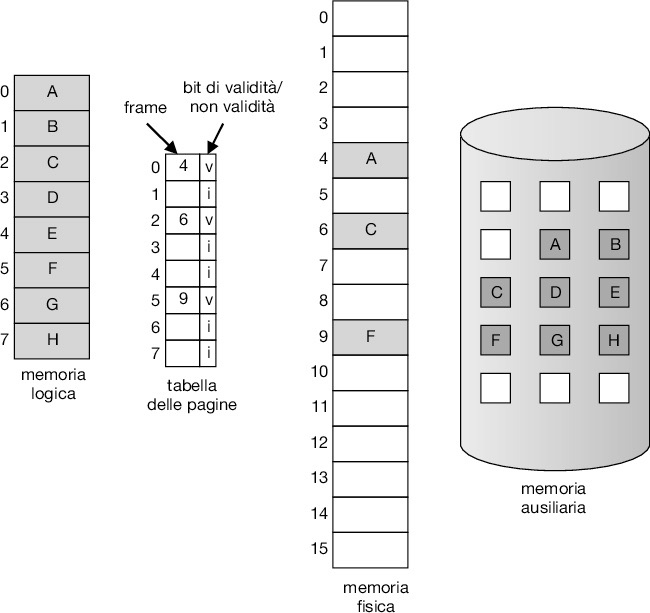
\includegraphics[width=0.25\linewidth]{images/table_of_pages_notAllInRam.png} \caption{Tabella delle pagine non presente totalmente in RAM} \label{fig:10.4} \end{figure}
\begin{figure}[h] \centering 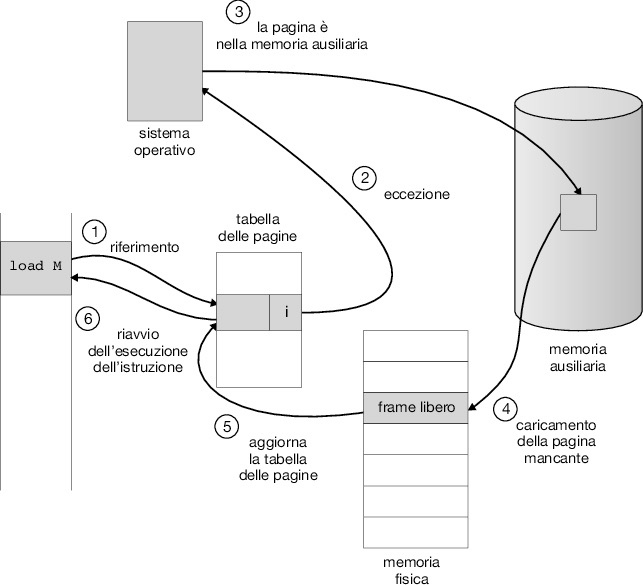
\includegraphics[width=0.25\linewidth]{images/page_fault_gestion.png} \caption{Gestione del Page Fault} \label{fig:10.5} \end{figure}

\section{Demand Paging}
\nt{
    Un processo può essere avviato senza che alcuna delle sue pagine sia inizialmente in Memoria Primaria (MP). Alla prima istruzione indirizzata dal Program Counter (PC), inizializzato dal Sistema Operativo (SO), si genera un \emph{page fault}, poiché il PC punta a un indirizzo di una pagina del processo non presente in MP. Questo schema è chiamato \emph{Pure Demand Paging}.
}

In alternativa, il SO può caricare preventivamente in MP almeno la pagina contenente la prima istruzione da eseguire.

\section*{Supporto Hardware per la Memoria Virtuale}

\nt{
    Per implementare la memoria virtuale è necessario un supporto hardware specifico:
    \begin{itemize}
        \item La tabella delle pagine deve includere un \emph{bit di validità} che l’hardware può testare per generare il \emph{page fault}.
        \item Le istruzioni devono essere ri-eseguibili in caso di \emph{page fault} oppure, alternativamente, l’hardware della CPU deve controllare la presenza in MP di tutti gli operandi prima di eseguire l'istruzione.
    \end{itemize}
}

\nt{
    Sebbene la paginazione possa essere aggiunta a qualsiasi sistema, la \emph{paginazione su richiesta} e, più in generale, la \emph{memoria virtuale}, richiedono un supporto hardware specifico.
}

\section*{Tempo di Accesso Effettivo}

Supponiamo di dover leggere un dato in MP:
\begin{itemize}
    \item \emph{ma} = tempo di accesso in MP se il dato è presente (es. 100-200 nanosecondi)
    \item \emph{p} = probabilità di un page fault
    \item \emph{eat} (effective access time) = 
    \[
    \text{eat} = [(1 - p) \times ma] + [p \times \text{tempo di gestione del page fault}]
    \]
\end{itemize}

\clm{Passi per la gestione di un page fault}{}{
    L’elenco completo dei passi necessari a gestire un page fault è descritto nel testo, ma le tre operazioni principali sono:
    \begin{enumerate}
        \item \textbf{Gestione del page fault}: richiede da 1 a 100 μsec.
        \item \textbf{Recupero della pagina mancante dalla Memoria Secondaria (MS)}: circa 8 millisecondi. Questo valore può variare a seconda del sistema, ma, se la memoria secondaria è su Hard Disk, l’ordine di grandezza è comunque di qualche millisecondo.
        \item \textbf{Riavvio del processo}: richiede da 1 a 100 μsec.
    \end{enumerate}
    \nt{I tempi per i punti 1 e 3 sono trascurabili rispetto al punto 2.}
}

\section*{Calcolo del Tempo di Accesso Effettivo}

Assumendo \textit{ma} = 200 nanosecondi, otteniamo (valori espressi in nanosecondi):
\[
\text{eat} = (1 - p) \times 200 + p \times 8.000.000 = 200 + p \times 7.999.800
\]

\ex{Calcolo con probabilità di page fault}{ 
    Se consideriamo \( p = 0.001 \) (un page fault ogni 1000 accessi), allora:
    \[
    \text{eat} = 200 + 0.001 \times 7.999.800 = 8.199,8 \text{ (circa 8,2 microsecondi)}
    \]
    \nt{In questo caso, l’esecuzione rallenta di oltre 40 volte!}
}

\qs{Degrado massimo del 10\%}{
    Per avere un degrado massimo del 10\%, la probabilità \( p \) deve rispettare la seguente disuguaglianza:
    \[
    \text{eat} = 220 > 200 + 8 \times 10^6 \times p
    \]
    \[
    20 > 8 \times 10^6 \times p
    \]
    \[
    p < 2,5 \times 10^{-6}
    \]
    Questo significa che non ci dovrebbero essere più di un page fault ogni 400.000 accessi in memoria.
}

\qs{400.000 accessi: sono molti o pochi?}{
    Se un processo esegue circa un milione di istruzioni, quanti accessi in RAM genera approssimativamente?
    \nt {
        1 milione di istruzioni = 1 milione di accessi in RAM (ogni istruzione richiede almeno un accesso in RAM).
        Alcune istruzioni possono richiedere più accessi in RAM, ma 1 milione è un buon punto di partenza.
    }
}

\nt{
    Il numero di page fault deve essere estremamente basso per evitare un aumento inaccettabile del tempo medio di esecuzione dei processi. Se il numero di page fault è elevato, il \textit{throughput} del sistema peggiora invece di migliorare.
}

\nt{
    È possibile intervenire anche sul tempo di gestione del page fault. Ad esempio:
    \begin{itemize}
        \item Usare pagine di grandi dimensioni, che possono ridurre il numero medio di page fault. (Perché?);
        \item Ottimizzare l'accesso alla Memoria Secondaria, anche se questa strategia presenta limiti, poiché implica comunque l’uso di hard disk. Si veda anche il capitolo 11, che tratta delle memorie a stato solido.
    \end{itemize}
}


\subsection{L'area di swap}


\dfn{Memoria Virtuale e Area di Swap}{
    Per funzionare, la memoria virtuale necessita di una porzione dedicata dell'Hard Disk, detta \textit{area di swap}.
}

\nt{
    Al momento dell'installazione del sistema operativo (SO), viene riservata una porzione del disco come area di swap ad uso esclusivo del SO. Questa area è gestita con meccanismi più semplici ed efficienti rispetto a quelli del file system:
    \begin{itemize}
        \item Le pagine dei processi non vengono salvate all'interno di file, evitando così l'uso dei file descriptor;
        \item Spesso, vengono utilizzati blocchi più grandi, con allocazione contigua, per migliorare le prestazioni di accesso (questo concetto sarà più chiaro nella parte sulla gestione della memoria secondaria).
    \end{itemize}
}

\clm{Utilizzo dell'Area di Swap}{}{
    Un modo semplice di usare l'area di swap consiste nel copiare l'eseguibile intero di un processo nell'area di swap all'avvio del processo:
    \begin{itemize}
        \item Il tempo di avvio del processo aumenta;
        \item Sono necessarie aree di swap di grandi dimensioni;
        \item Tuttavia, la gestione dei page fault è più veloce, poiché il recupero delle pagine è più rapido una volta che queste sono già nell'area di swap, senza passare attraverso il file system.
    \end{itemize}
}

\clm{Uso Alternativo dell'Area di Swap}{}{
    In alternativa, le pagine dell’eseguibile o di eventuali file di dati possono essere lette direttamente dal file system:
    \begin{itemize}
        \item Utile quando occorre limitare le dimensioni dell'area di swap;
        \item L’avvio dei processi è più veloce;
        \item L'esecuzione può risultare più lenta rispetto all'uso della swap.
    \end{itemize}
}

Notiamo che l’area di swap sembra meno utile se viene utilizzata solo per ospitare gli eseguibili e gli eventuali dati in input prima di avviare i processi. 
Funzione Principale dell'Area di Swap
L’area di swap viene utilizzata soprattutto per:
\begin{itemize}
    \item Liberare spazio in memoria primaria (MP) per ospitare pagine mancanti, caricate in RAM in risposta a un page fault.
\end{itemize}


\nt{
    In effetti, se ci fosse sempre un frame libero, una pagina verrebbe caricata in MP solo la prima volta che viene indirizzata. Tuttavia, l'idea principale della memoria virtuale è di:
    \begin{itemize}
        \item Permettere l'esecuzione di un processo più grande della memoria primaria disponibile.
        \item Consentire l'esecuzione simultanea di processi che, nel complesso, richiedono più spazio di quello disponibile in RAM.
    \end{itemize}
}

Si consideri la situazione in cui due processi occupano più spazio di quello disponibile in memoria principale (cfr. Fig. 10.9).
\begin{figure}[h] \centering 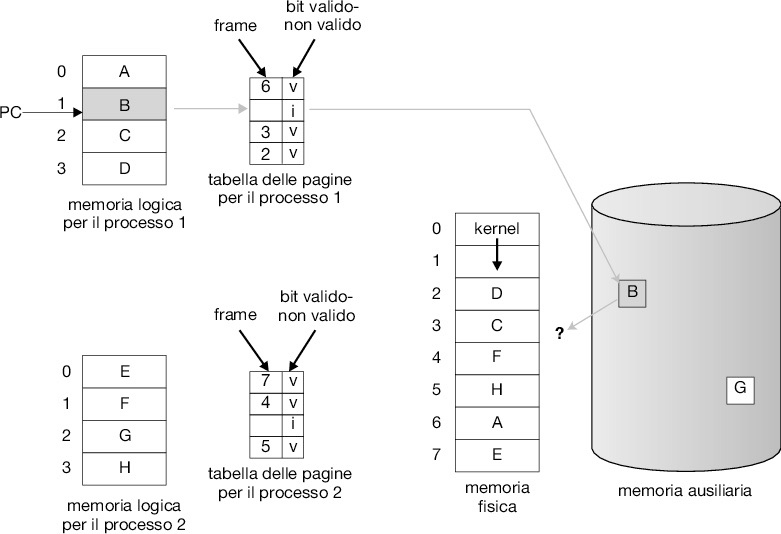
\includegraphics[width=0.5\linewidth]{images/swap_disegno.png} \caption{Swap 10.9} \label{fig:10.9} \end{figure}
Dunque, se si verifica un page fault e tutti i frame della RAM sono occupati, occorre liberarne uno rimuovendo la
agina che ospita, che prende il nome di \textbf{pagina vittima}.\\
Se la pagina vittima contiene dati modificati o fa parte dello stack o della heap di un processo, la pagina va salvata nell’area di swap, in modo che possa essere recuperata quando il processo a cui appartiene vi farà riferimento.\\
Le pagine di codice non devono essere salvate, tanto ce n’è comunque una copia nel file system, ma se erano state copiate inizialmente nell’area di swap potranno poi essere recuperate più velocemente se riferite di nuovo.\\


\section{Sostituzione delle pagine}
\qs{Cosa succede se si verifica un page fault e non c'è alcun frame libero in RAM?}{
    In questo caso, il sistema operativo esegue i seguenti passi:
    \begin{itemize}
        \item Seleziona una pagina "vittima" da rimuovere.
        \item Salva la pagina vittima nell'area di swap (se necessario).
        \item Carica la pagina mancante nel frame liberato.
    \end{itemize}
}

\nt{
Questa procedura è simile al concetto di \textit{swapping} di processi interi. Tuttavia, con la memoria virtuale, il sistema sposta tra RAM e hard disk solo frammenti di processo, ossia una pagina alla volta.
}

\nt{
Se la pagina vittima non è stata modificata da quando è stata caricata in RAM, si può evitare di salvarla nuovamente su disco, poiché ne esiste già una copia in memoria secondaria.
}

Se la pagina vittima è stata modificata, il tempo di gestione del page fault raddoppia poiché è necessario sia salvarla che caricare la nuova pagina. Un \textit{dirty bit} associato a ciascuna entry della tabella delle pagine (PT) può semplificare il processo: il \textit{dirty bit} viene settato a 1 dall’hardware della CPU la prima volta che la pagina viene modificata in RAM. In questo modo, solo le pagine vittima con il \textit{dirty bit} a 1 devono essere salvate in memoria secondaria.

\clm{Modifica e salvataggio delle pagine in memoria virtuale}{}{
    Solo le pagine di dati (stack e heap) possono essere modificate e, quindi, avere il \textit{dirty bit} a 1. Le pagine di codice, essendo accedute solo in lettura, non necessitano di essere salvate nell'area di swap se scelte come pagine vittima. Inoltre, se il codice era stato inizialmente copiato nell'area di swap, riportare le pagine di codice in RAM è più rapido rispetto al caricamento dall'eseguibile nel file system.
}

\nt{
La gestione della sostituzione delle pagine è fondamentale per consentire l'esecuzione di programmi più grandi della memoria primaria disponibile. Tuttavia, ciò comporta due problemi rilevanti:
\begin{itemize}
    \item \textbf{Scelta della pagina da sostituire}: Quale pagina scegliere come vittima?
    \item \textbf{Allocazione dei frame}: Quanti frame assegnare a ciascun processo? (aspetto che verrà discusso in seguito)
\end{itemize}
Il metodo utilizzato per risolvere questi problemi influisce notevolmente sulle prestazioni di esecuzione dei processi.
}

\begin{figure}[h] \centering 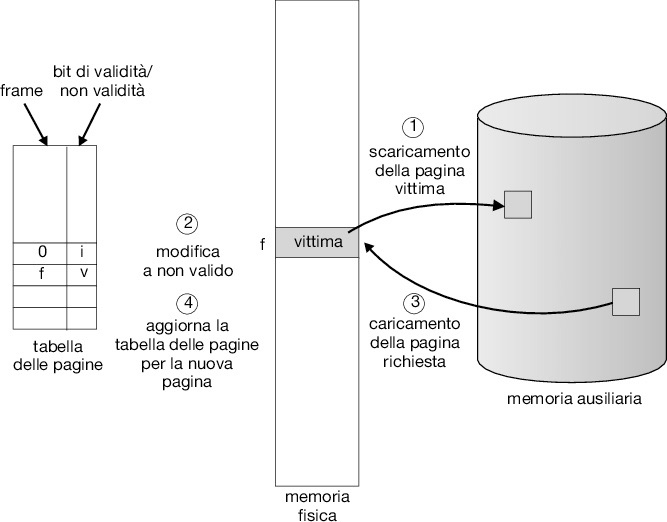
\includegraphics[width=0.50\linewidth]{images/sostituzione_di_pagina.png} \caption{Sostituzione di pagina} \label{fig:10.10} \end{figure}

\subsection{Algoritmi di sostituzione delle pagine}
Se una pagina vittima appena rimossa viene nuovamente indirizzata dal processo a cui appartiene, si verifica un \textit{page fault} e la pagina deve essere ricaricata in memoria principale. In questo caso, parte del lavoro viene sprecato.\\
Al contrario, se la pagina vittima scelta non verrà mai più utilizzata, non sarà necessario ricaricarla in memoria, ottimizzando l'uso della memoria primaria.\\

\clm{Obiettivo degli algoritmi di sostituzione delle pagine}{}{
    Un buon algoritmo di sostituzione minimizza il numero di \textit{page fault}. In letteratura, questi algoritmi sono spesso chiamati \textit{algoritmi di rimpiazzamento delle pagine}.
}

\qs{Come possiamo valutare l'efficacia di diversi algoritmi di sostituzione delle pagine?}{
    Si può valutare l'efficacia tramite sequenze di riferimenti in memoria principale:
    \begin{itemize}
        \item \textbf{generate casualmente}, oppure
        \item \textbf{generate dall'esecuzione di programmi reali}.
    \end{itemize}
    Non interessa l’indirizzo esatto dell'istruzione, ma solo il numero della pagina indirizzata, ignorando quindi l’offset.
}

\ex{Esempio di sequenza di riferimento}{
    Supponiamo che la sequenza di riferimento sia:
    \[
    10, 7, 4, 5, 6, 1, 10, 4, \dots
    \]
    Durante l’esecuzione, la CPU ha generato una sequenza di indirizzi logici che indirizzano le pagine in quest'ordine.
}

\qs{Quanti \textit{page fault} genera questa sequenza di riferimento?}{
    Supponiamo di avere a disposizione un solo frame in memoria. Con questa ipotesi, la sequenza provoca 8 \textit{page fault}.
    
    Consideriamo invece la seguente sequenza:
    \[
    10, 7, 7, 7, 4, 5, 5, 5, 5, 6, 1, 10, 10, 10, 10, 4
    \]
    Anche questa sequenza causa 8 \textit{page fault}, poiché i riferimenti consecutivi alla stessa pagina non generano nuovi \textit{page fault} dopo che la pagina è stata caricata in memoria primaria.
}

\nt{
Pertanto, le sequenze:
\[
10, 7, 4, 5, 6, 1, 10, 4
\]
e
\[
10, 7, 7, 7, 4, 5, 5, 5, 5, 6, 1, 10, 10, 10, 10, 4
\]
sono equivalenti per quanto riguarda la valutazione della bontà di un algoritmo di sostituzione.
}

\nt{
Il numero di \textit{page fault} generati da una sequenza per un dato algoritmo di sostituzione dipende anche dal numero di frame disponibili. Intuitivamente, all’aumentare dei frame disponibili, il numero di \textit{page fault} tende a ridursi — ma come vedremo, ciò non accade sempre!
}
\begin{figure}[h] \centering 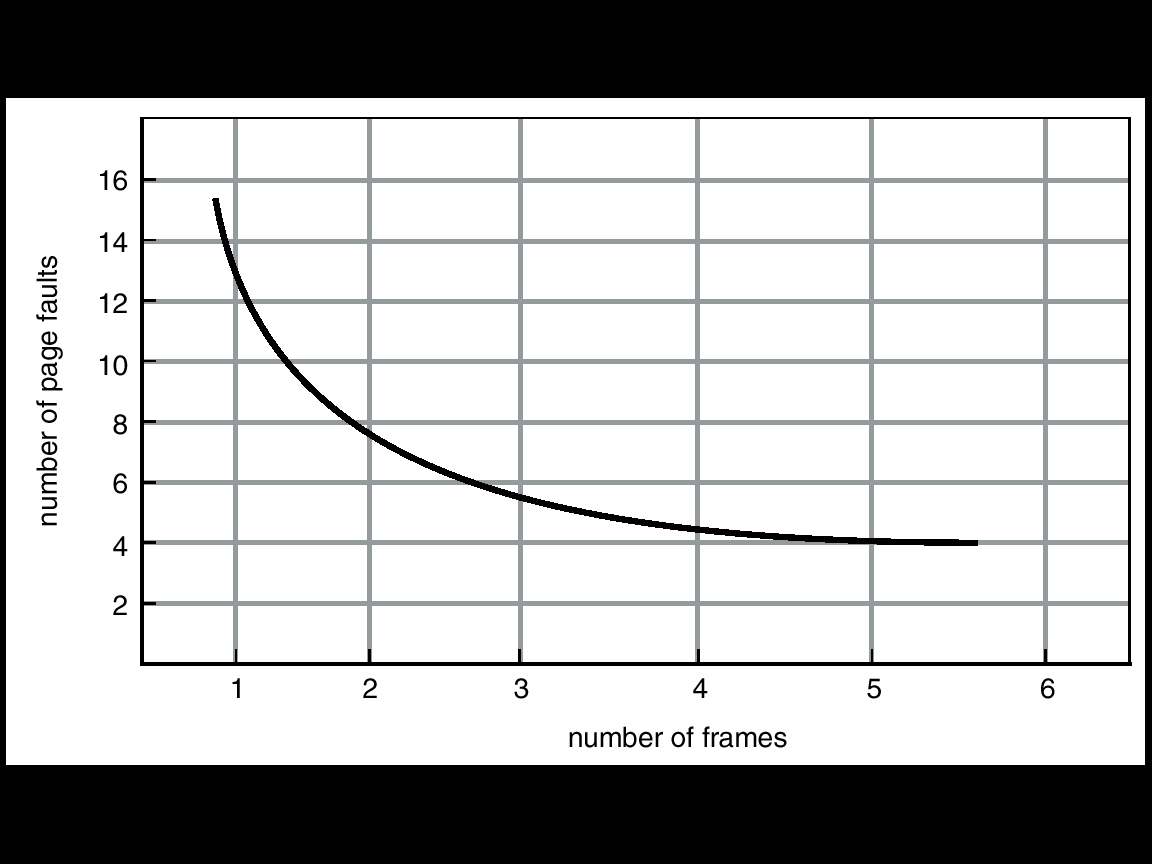
\includegraphics[width=0.50\linewidth]{images/page_faultGraph.png} \caption{Grafico dei page fault} \label{fig:5.4} \end{figure}

\subsection{Sostituzione delle pagine secondo l’ordine d’arrivo (FIFO)}
Nel seguito, assumeremo che a ogni processo venga assegnato un numero prestabilito di frame e che la scelta della pagina vittima avvenga esclusivamente tra le pagine del processo stesso. Questa politica prende il nome di sostituzione \textbf{locale} delle pagine.\\
Assumiamo inoltre uno schema di \textit{paginazione su richiesta puro}: quando un processo inizia, nessuna delle sue pagine è in RAM, e quindi il primo riferimento a una pagina qualsiasi genera un \textit{page fault}.\\

\dfn{Algoritmo FIFO}{
    L’algoritmo \textbf{FIFO} (First In, First Out) sceglie come pagina vittima quella presente da più tempo in memoria principale. Questo approccio è semplice da implementare ma non garantisce sempre buone prestazioni:
    \begin{itemize}
        \item Se la pagina vittima contiene codice di inizializzazione usato solo all'inizio, allora la rimozione va bene, poiché la pagina non verrà più utilizzata.
        \item Tuttavia, se la pagina contiene una variabile usata per tutta l’esecuzione del codice o una procedura richiamata frequentemente, la rimozione potrebbe rivelarsi inefficiente.
    \end{itemize}
}

\ex{Esempio di FIFO}{
    Consideriamo la sequenza di riferimenti:
    \[
    7, 0, 1, 2, 0, 3, 0, 4, 2, 3, 0, 3, 2, 1, 2, 0, 1, 7, 0, 1
    \]
    Con 3 frame disponibili, questa sequenza produce 15 \textit{page fault} (vedi Fig. 10.12).
}
\begin{figure}[h] \centering 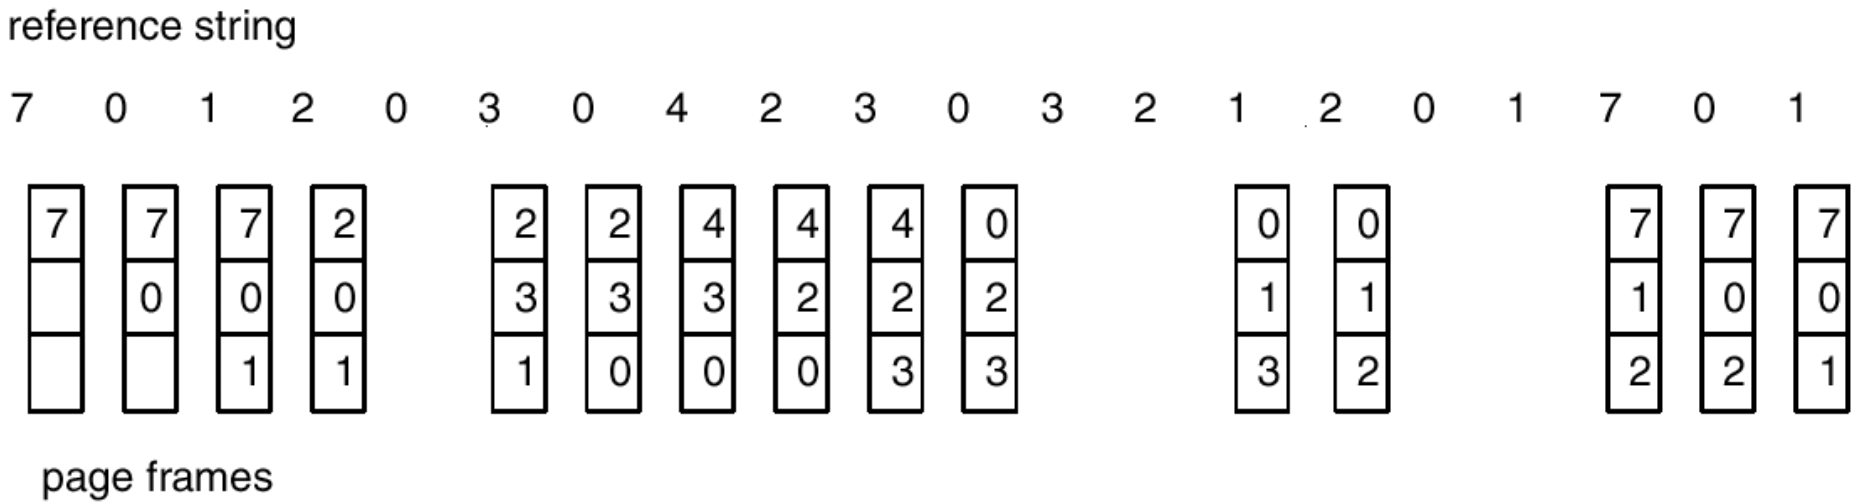
\includegraphics[width=0.50\linewidth]{images/fifo_page_fault.png} \caption{10.12} \label{fig:10.12} \end{figure}

\nt{
L'algoritmo FIFO è affetto dalla cosiddetta \textit{Anomalia di Belady}: in alcuni casi, aumentando il numero di frame, il numero di \textit{page fault} può paradossalmente aumentare!
}

\ex{Anomalia di Belady}{
    Consideriamo la seguente stringa di riferimento:
    \[
    1, 2, 3, 4, 1, 2, 5, 1, 2, 3, 4, 5
    \]
    In alcuni casi, aumentando il numero di frame, il numero di \textit{page fault} prodotti può aumentare (vedi Fig. 10.13). È importante notare che questo fenomeno si verifica solo per alcune specifiche sequenze di riferimento.
}

\begin{figure}[h] \centering 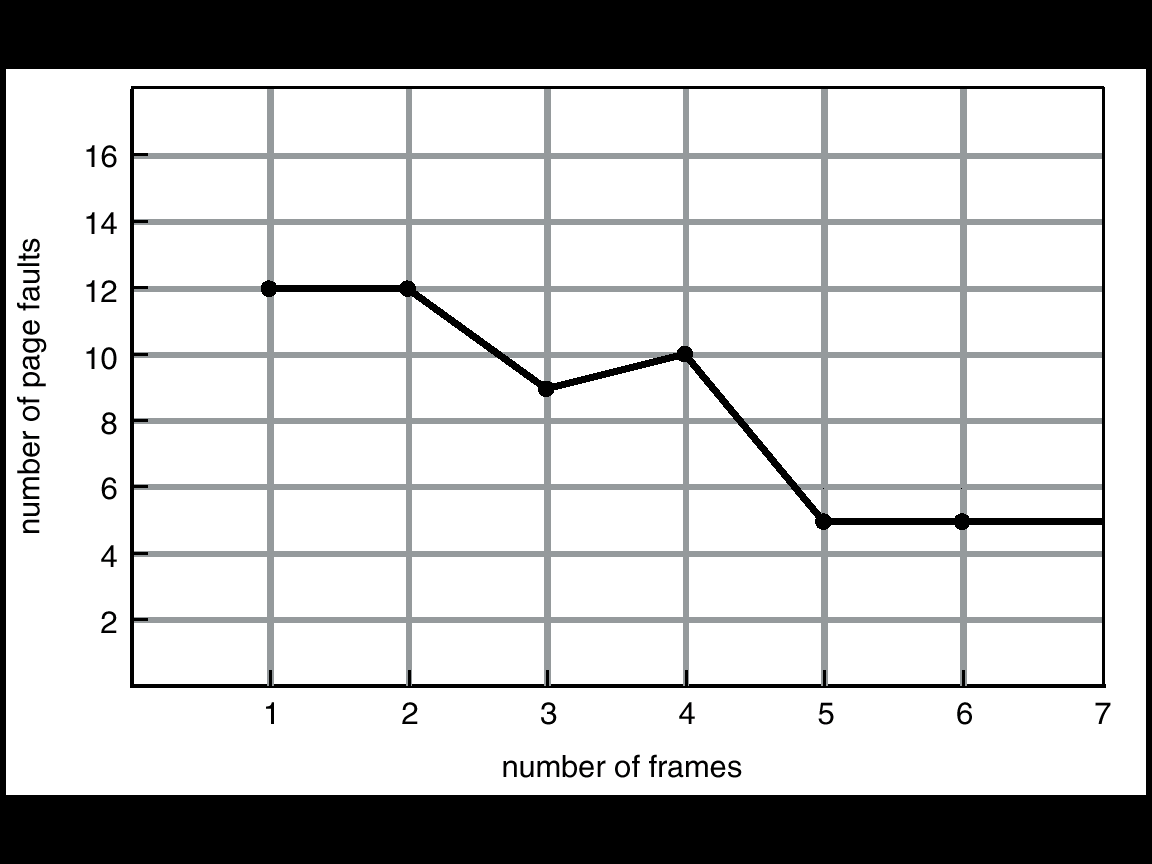
\includegraphics[width=0.33\linewidth]{images/belady_anomaly.png} \caption{10.13} \label{fig:10.13} \end{figure}

\dfn{Algoritmo OPT (o MIN)}{
    L’algoritmo \textbf{OPT}, o \textbf{MIN}, seleziona come vittima la pagina che verrà utilizzata più avanti nel tempo rispetto a tutte le altre pagine attualmente in memoria. Questo algoritmo garantisce il numero minimo di \textit{page fault} per un dato numero di frame, evitando l'anomalia di Belady.
    
    Tuttavia, \textbf{OPT non è implementabile} in un sistema reale, poiché richiederebbe una conoscenza anticipata dell’uso delle pagine. Viene usato solo come termine di paragone per valutare le prestazioni di altri algoritmi.
}

\ex{Esempio di OPT}{
    Utilizzando l'algoritmo OPT con 3 frame, la sequenza:
    \[
    7, 0, 1, 2, 0, 3, 0, 4, 2, 3, 0, 3, 2, 1, 2, 0, 1, 7, 0, 1
    \]
    produce 9 \textit{page fault} (vedi Fig. 10.14).
}

\subsection{Algoritmo LRU (Least Recently Used)}
\nt{
L’algoritmo OPT è ideale perché sceglie come pagina vittima quella che non verrà più utilizzata nel futuro, ma ovviamente non è implementabile. Un tentativo di approssimazione di questo comportamento è l’algoritmo \textbf{LRU} (Least Recently Used), che seleziona come vittima la pagina che non è stata usata da più tempo.
}

\dfn{Algoritmo LRU}{
    L'algoritmo \textbf{LRU} non soffre dell'anomalia di Belady e si avvicina molto a OPT, ma ha il difetto di essere difficile da implementare in modo efficiente. In pratica, LRU guarda al passato (anziché al futuro) per determinare quale pagina rimuovere. Questo approccio funziona bene nella maggior parte dei casi, ma è più complesso da implementare.
}

\ex{Esempio di LRU}{
    Consideriamo la seguente sequenza di riferimenti:
    \[
    7, 0, 1, 2, 0, 3, 0, 4, 2, 3, 0, 3, 2, 1, 2, 0, 1, 7, 0, 1
    \]
    Con 3 frame disponibili, l'algoritmo LRU produce 12 \textit{page fault} (vedi Fig. 10.15).
}
\begin{figure}[h] \centering 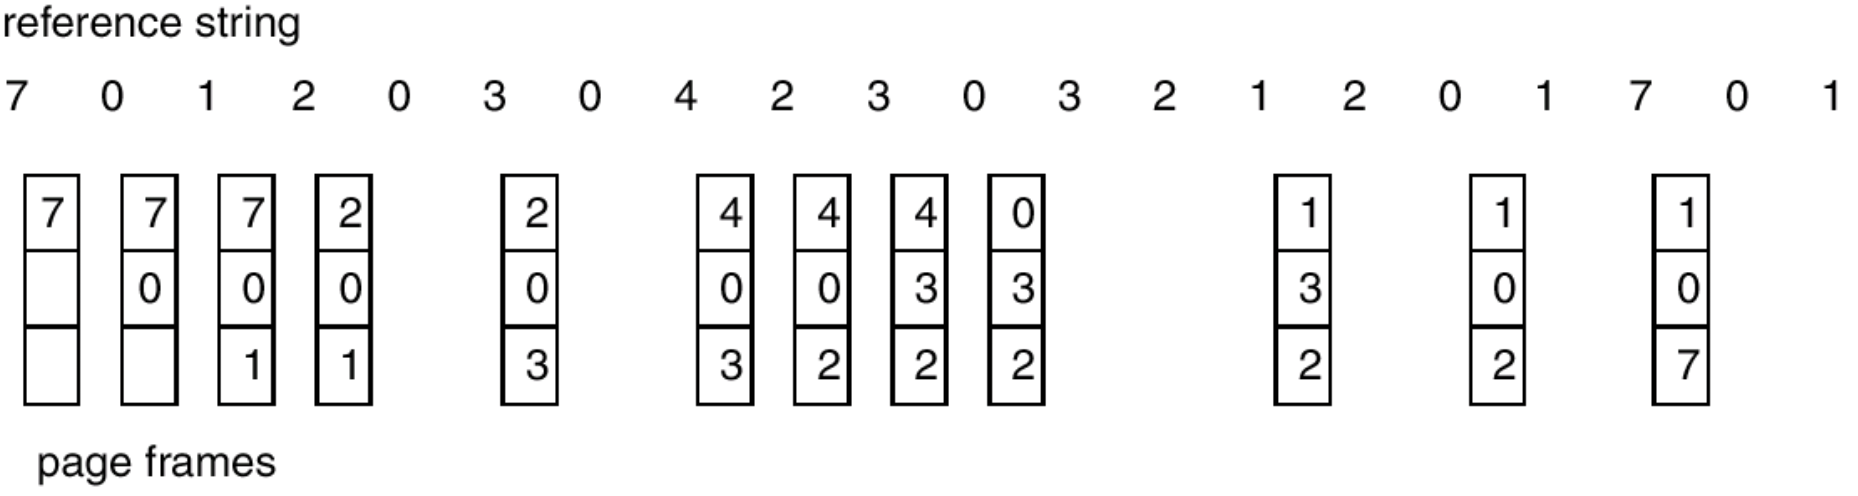
\includegraphics[width=0.50\linewidth]{images/lru_pages_alg.png} \caption{10.15} \label{fig:10.15} \end{figure}
L’implementazione dell'algoritmo LRU richiederebbe un supporto hardware da parte della CPU che, purtroppo, non è disponibile nelle architetture moderne. Tuttavia, esistono approcci che utilizzano un supporto hardware più semplice per approssimare LRU in modo accettabile.

\dfn{Reference Bit}{
    Molti processori forniscono un \textit{reference bit}, un bit associato a ciascuna pagina nella Page Table di un processo. Quando un processo inizia, tutti i reference bit delle sue pagine sono inizializzati a 0 dal sistema. 
    \begin{itemize}
        \item Quando una pagina viene indirizzata (sia in lettura che in scrittura), l'hardware imposta a 1 il reference bit di quella pagina.
        \item In questo modo, possiamo sapere quali pagine sono state utilizzate di recente, anche se non sappiamo l'ordine esatto di accesso.
    \end{itemize}
}

\subsubsection{Algoritmo LRU Seconda Chance}
Partendo da un algoritmo FIFO, in caso di \textit{page fault} il sistema operativo esamina la pagina che è entrata per prima in RAM. Se il reference bit di questa pagina è 0, essa viene scelta come pagina vittima. Se invece il reference bit è 1, la pagina riceve una "seconda chance": il suo reference bit viene azzerato e viene trattata come se fosse appena entrata in memoria.

\dfn{Algoritmo della Seconda Chance}{
    L'algoritmo della seconda chance funziona come segue:
    \begin{itemize}
        \item Se il reference bit di una pagina è 0, la pagina viene selezionata come vittima.
        \item Se il reference bit è 1, il bit viene azzerato e la pagina viene spostata in fondo alla coda FIFO.
    \end{itemize}
    Se in una sequenza di sostituzioni tutte le pagine hanno il reference bit impostato a 1, l'algoritmo riprende a esaminare la prima pagina della coda (quella entrata per prima in RAM) e la seleziona come vittima, tornando di fatto a un algoritmo FIFO.
}
Se una pagina viene riferita frequentemente, il suo reference bit rimarrà a 1 per la maggior parte del tempo, riducendo la probabilità che venga selezionata come vittima. Questo algoritmo è una buona approssimazione di LRU ed è decisamente più efficiente di una gestione completa di LRU in hardware.\\
Se “next victim” non viene riferita prima di una seconda chiamata dell’algoritmo, il suo reference bit resta a 0, quindi non è stata riferita di recente, e diviene quindi una buona candidata alla sostituzione.\\

\begin{figure}[h] \centering 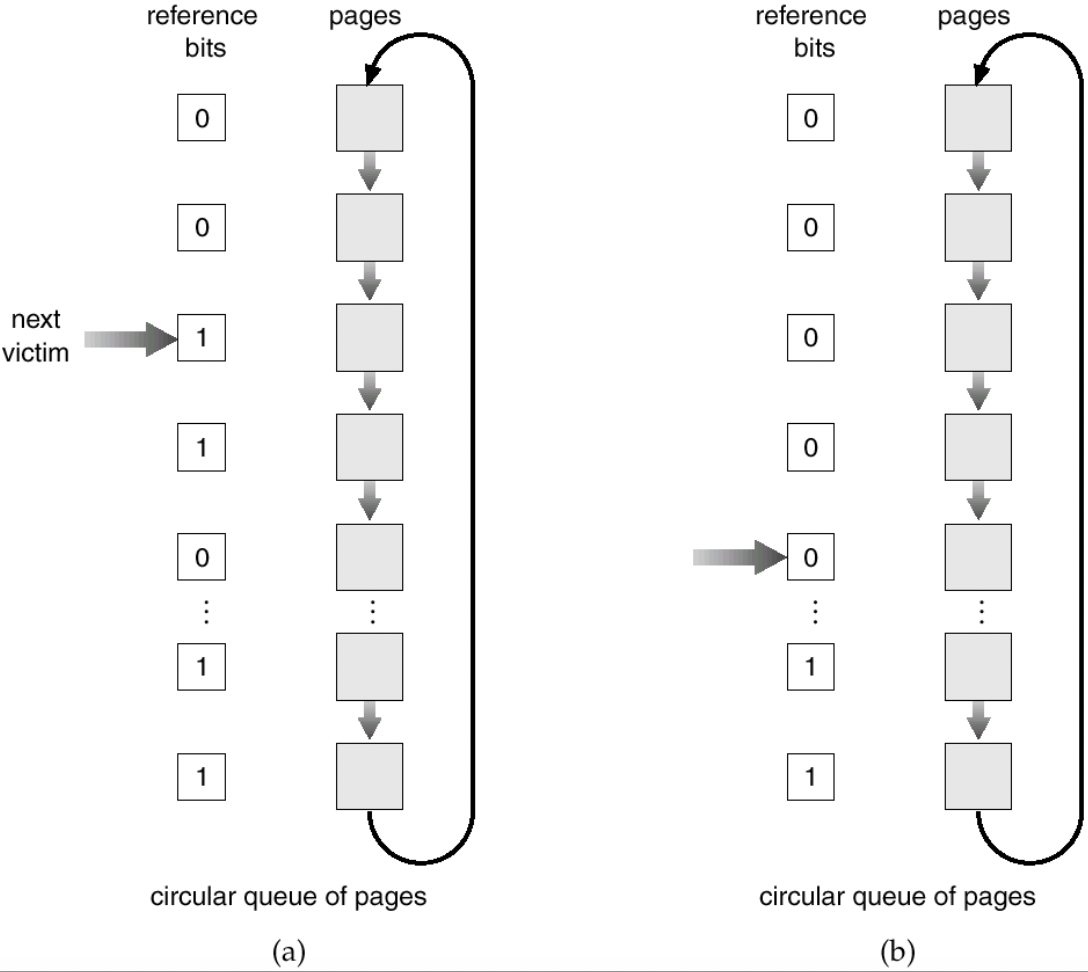
\includegraphics[width=0.25\linewidth]{images/second_chanceQueue.png} \caption{10.17} \label{fig:10.17} \end{figure}

\subsection{Algoritmo Seconda Chance con Dirty Bit} 
Quando l'hardware fornisce sia il \textit{reference bit} che il \textit{dirty bit}, le pagine possono essere classificate in quattro gruppi, ognuno dei quali ha una priorità diversa per essere sostituito:

\dfn{Classificazione delle Pagine}{
    Le pagine sono raggruppate in base a due bit: il \textit{reference bit} e il \textit{dirty bit}.
    \begin{itemize}
        \item \textbf{(0, 0)}: La pagina non è stata utilizzata di recente e non è stata modificata. È la migliore da rimpiazzare.
        \item \textbf{(1, 0)}: La pagina è stata utilizzata di recente, ma non è stata modificata. È una buona candidata, ma meno preferibile rispetto a quella (0, 0).
        \item \textbf{(0, 1)}: La pagina non è stata utilizzata di recente, ma è stata modificata. È meno buona da sostituire, in quanto dovrà essere salvata in memoria secondaria per non perdere le modifiche.
        \item \textbf{(1, 1)}: La pagina è stata utilizzata di recente e modificata. È la peggiore da sostituire, poiché richiede di essere salvata in memoria secondaria prima di essere rimossa.
    \end{itemize}
}
Il principio di sostituzione applicato in questo algoritmo è simile a quello della "Seconda Chance". In questo caso, si seleziona come vittima la prima pagina che appartiene alla classe migliore non vuota (quella con il valore \textbf{(0, 0)} se disponibile, poi \textbf{(1, 0)}, e così via).

\dfn{Algoritmo di Sostituzione con Reference e Dirty Bit}{
    L'algoritmo, che si basa su questa classificazione delle pagine, è utilizzato in molti sistemi operativi Unix e in macOS. La scelta della pagina da rimpiazzare dipende dallo stato combinato dei bit di riferimento e di modifica, con la preferenza per le pagine meno utilizzate e non modificate.
}

\section{Allocazione dei Frame}
In un sistema multiprogrammato, la distribuzione dei frame disponibili tra i processi può essere gestita in vari modi:

\dfn{Strategie di Distribuzione dei Frame}{
    \begin{itemize}
        \item \textbf{Allocazione uniforme}: Ogni processo riceve lo stesso numero di frame. Ad esempio, se ci sono $n$ frame e $p$ processi, ogni processo ottiene $n/p$ frame.
        \item \textbf{Allocazione proporzionale}: I frame vengono distribuiti in base alle dimensioni di ogni processo. Ad esempio, se i processi sono di dimensioni diverse, i processi più grandi riceveranno più frame.
        \item \textbf{Allocazione proporzionale in base alla priorità}: La distribuzione dei frame tiene conto della priorità dei processi. I processi con priorità più alta ricevono più frame.
        \item \textbf{Allocazione con riserva di frame}: Alcuni frame devono essere tenuti liberi per consentire l'ingresso di nuovi processi nel sistema.
    \end{itemize}
}

\dfn{Esempio di Allocazione Proporzionale}{
    Se abbiamo 11 frame disponibili e i processi P1, P2 e P3 hanno dimensioni rispettive di 4, 6 e 12 pagine, la distribuzione dei frame sarà:
    \begin{itemize}
        \item P1: 2 frame,
        \item P2: 3 frame,
        \item P3: 6 frame.
    \end{itemize}
}
Nel caso dell'allocazione proporzionale in base alla priorità, il numero di frame assegnati a ciascun processo dipenderà dalla priorità relativa dei processi (e in alcuni casi dalle loro dimensioni).\\

\dfn{Allocazione dei Frame e Grado di Multiprogrammazione}{
    \nt{
    Qualunque schema di allocazione venga scelto, il numero di frame assegnato a ciascun processo cambierà in funzione del grado di multiprogrammazione. 
    }
}

\dfn{Strategie di Selezione della Vittima per la Rimozione}{
    In caso di page fault, bisogna scegliere quale pagina rimuovere dalla memoria principale:
    \begin{itemize}
        \item \textbf{Allocazione globale}: La vittima è scelta fra tutte le pagine in memoria principale, esclusi i frame utilizzati dal sistema operativo. Questo approccio potrebbe rimuovere una pagina di un altro processo rispetto a quello che ha causato il page fault.
        \item \textbf{Allocazione locale}: La vittima è scelta fra le pagine del processo che ha causato il page fault, mantenendo costante il numero di frame allocato a ciascun processo.
    \end{itemize}
}

\wc{Problemi}{
\textbf{Problemi dell'Allocazione Globale}: La strategia globale rende il turnaround di un processo fortemente dipendente dal comportamento degli altri processi, con un elevato rischio di variazione nelle prestazioni da un'esecuzione all'altra. 

\textbf{Problemi dell'Allocazione Locale}: Se un processo riceve troppi frame, ciò può ridurre il throughput complessivo del sistema, poiché gli altri processi avranno meno frame disponibili e genereranno più page fault.
}

\nt {
Si è visto sperimentalmente che l’allocazione globale fornisce in genere un throughput maggiore e riesce a gestire la multiprogrammazione in maniera più flessibile.\\
L’allocazione globale è di solito preferita per sistemi time sharing, in cui molti utenti possono usare contemporaneamente il sistema.\\
I sistemi Windows usano l’allocazione locale, mentre Linux e Solaris usano l’allocazione globale delle pagine.\\
}

\subsection{Thrashing (attività di paginazione degenere)}
\nt{
Consideriamo un sistema in cui, in un dato momento, ogni processo ha a disposizione un numero ridotto di frame, cioè ogni processo ha in memoria principale (MP) un numero di pagine inferiore rispetto al numero totale di pagine di cui è composto. Supponiamo anche di adottare una allocazione globale dei frame. Va sottolineato che il problema del \textbf{thrashing} si può verificare anche nel caso di allocazione locale dei frame. 
}

\dfn{Probabilità di Page Fault}{
    Con poche pagine in RAM per processo, la probabilità che ogni processo generi un page fault è alta. In seguito a un page fault, una pagina vittima viene rimossa dalla memoria principale (MP), probabilmente da un altro processo. 

    Questo altro processo, a sua volta, avrà ancora meno pagine in memoria, aumentando ulteriormente la probabilità che anche esso generi un page fault a breve. Si innesca così un circolo vizioso in cui:
    \begin{itemize}
        \item Ogni processo genera continuamente page fault,
        \item I frame vengono "rubati" tra i vari processi,
        \item La probabilità di page fault aumenta continuamente.
    \end{itemize}
}

\dfn{Thrashing}{
    Questo fenomeno è noto come \textbf{thrashing}, che si verifica quando il sistema tenta di aumentare eccessivamente il grado di multiprogrammazione, ossia cercando di eseguire più processi contemporaneamente per sfruttare al massimo la CPU e incrementare il throughput del sistema. 

    Tuttavia, oltre una certa soglia, i processi passano più tempo a gestire i page fault generati che ad eseguire realmente il loro lavoro. Di conseguenza, la \textit{utilizzazione della CPU} diminuisce drasticamente e il \textit{throughput} del sistema crolla. 
}

\dfn{Relazione tra Grado di Multiprogrammazione e Thrashing}{
    Il grado di multiprogrammazione è direttamente legato al rischio di thrashing. Aumentando il numero di processi che cercano di essere eseguiti contemporaneamente, cresce anche la probabilità che ognuno di essi abbia pochi frame disponibili. Questo può portare a una situazione in cui il sistema è sopraffatto dalla gestione dei page fault, riducendo di fatto l'efficienza complessiva. 

    La relazione tra grado di multiprogrammazione e throughput diventa inversamente proporzionale oltre una certa soglia, con l'aumento della multiprogrammazione che inizialmente porta a un miglioramento delle prestazioni, ma che successivamente provoca un forte degrado delle stesse a causa del thrashing.
}

\begin{figure}[h] \centering 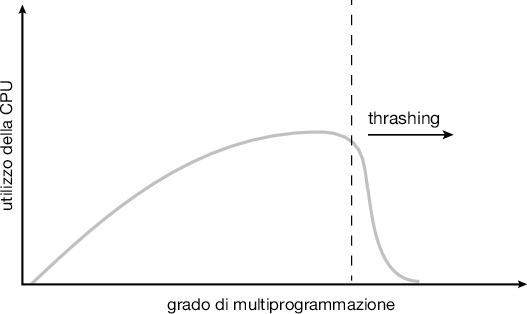
\includegraphics[width=0.55\linewidth]{images/tharsing_multiporgGraph.png} \caption{10.20} \label{fig:10.20} \end{figure}

\subsection{Cause del Thrashing}
Se il livello di utilizzo della CPU di un sistema è troppo basso, lo si può alzare aumentando in grado di permettendo a più utenti di connettersi, e/o di lanciare un maggior numero di processi. In questo modo però, i nuovi processi incominciano a sottrarre pagine ai processi già presenti, per “farsi un po' di spazio”. Fino ad un certo punto l’aumento di processi è ben tollerato dal sistema, poiché ciascun processo ha comunque una quantità sufficiente di frame a disposizione da poter girare senza generare troppi page fault. Ma se si esagera, ci si può avvicinare alla soglia del thrashing: molti processi incominciano a generare dei page fault e, come conseguenza, vengono tolti dalla RQ e messi in una coda di wait in attesa della pagina mancante. Risultato? La RQ si svuota, e il livello di utilizzo della CPU scende. Beh, ma se la CPU è sotto-utilizzata, si può lanciare qualche altro processo, o permettere a qualche altro utente di collegarsi... E la situazione non fa che peggiorare!.\\
Nei moderni sistemi time-sharing, il ciclo perverso è spesso innescato dagli utenti, che lanciano altri programmi senza attendere la fine di quelli già in esecuzione, sperando così di aumentare la percentuale del tempo di CPU globale che riescono ad usare a loro vantaggio.\\
In definitiva quindi, il thrashing è una sorta di “ingolfamento” del sistema: vogliamo sfruttarlo al meglio “iniettando” più e più processi nel sistema, fino ad arrivare ad un punto in cui i processi si ostacolano a vicenda.\\
La soluzione giusta sarebbe di diminuire il grado di multiprogrammazione temporaneamente, in modo che i processi non rimossi dalla MP abbiano il tempo di terminare correttamente prima di far (ri)partire gli altri.\\


\subsection{Come combattere il Thrashing}
In definitiva, quindi, il \textit{thrashing} rappresenta una sorta di “ingolfamento” del sistema: si tenta di sfruttare al massimo le risorse “iniettando” più processi possibili, ma si finisce per raggiungere un punto in cui i processi si ostacolano a vicenda.

\nt{
    La soluzione ottimale consiste nel ridurre temporaneamente il grado di multiprogrammazione. Così facendo, i processi ancora presenti in memoria possono completare correttamente la loro esecuzione, prima di permettere l'avvio (o il riavvio) di altri processi.
}

\clm{Frequenza accettabile dei page fault}{}{
    È possibile stabilire, ad esempio in base ad osservazioni sperimentali, un livello “accettabile” di frequenza di page fault, per raggiungere le prestazioni desiderate:
    \begin{itemize}
        \item \textbf{Se la frequenza osservata è troppo bassa}, si possono rimuovere alcuni frame dai processi e aumentare il grado di multiprogrammazione.
        \item \textbf{Se la frequenza osservata è troppo alta}, occorre diminuire il grado di multiprogrammazione e redistribuire i frame liberati tra i processi ancora attivi.
    \end{itemize}
}

\nt{
    Il \textit{thrashing} può essere prevenuto monitorando attentamente la frequenza dei page fault (come illustrato in figura 10.23).
}

\begin{figure}[h] \centering 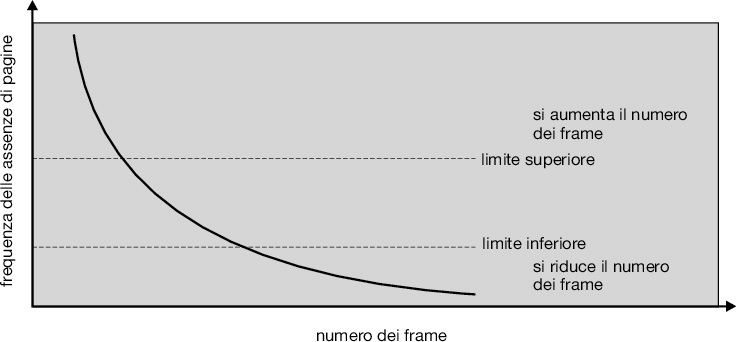
\includegraphics[width=0.50\linewidth]{images/frequenctOfPageFault.png} \caption{Frequenza dei page fault} \label{fig:10.23} \end{figure}

Adottare una politica di sostituzione locale può contribuire a ridurre il rischio di thrashing, poiché i processi non possono sottrarsi le pagine tra loro. Se un singolo processo entra in thrashing, non danneggia gli altri, sebbene possa utilizzare intensivamente le risorse di I/O su disco.

Tuttavia, se si assegnano troppi pochi frame a ciascun processo per aumentare eccessivamente il grado di multiprogrammazione, esiste il rischio che tutti i processi entrino in thrashing.

\cor{Prevenzione ottimale del thrashing}{
    La migliore prevenzione del thrashing è dotare il sistema di una quantità sufficiente di memoria principale.
}

\section{Dimensioni delle pagine}
Sono sempre potenze di $2$; ma quanto dovrebbero essere grandi? 

\begin{itemize}
    \item \textbf{Pagine piccole} implicano:
    \begin{itemize}
        \item Tabelle delle pagine (PT) più grandi;
        \item meno frammentazione interna;
        \item peggiori prestazioni nell’uso dell'HD, poiché il \textit{seek} e la latenza del disco sono costanti (si vedrà meglio nel Capitolo 11);
        \item in generale, un maggior numero di page fault (immaginiamo pagine di un solo byte in pure demand paging).
    \end{itemize}
    
    \item \textbf{Pagine grandi} presentano le considerazioni opposte.
\end{itemize}

A causa della diminuzione del costo della RAM e dell’aumento degli spazi di indirizzamento fisico disponibili, la tendenza è quella di usare pagine sempre più grandi. Negli anni ’80, $4$ Kbyte era considerata la dimensione massima accettabile di una pagina, mentre oggi tale valore è normale, e spesso anche superato. 

\nt{
    L'aumento costante della quantità di RAM nei sistemi moderni ha fatto sì che, nel tempo, il problema del \textit{thrashing} e, più in generale, le problematiche legate alla memoria virtuale abbiano un impatto minore sulle prestazioni complessive dei sistemi.
}

\subsection{Struttura dei programmi}
Il modo in cui i programmi utilizzano i dati influisce significativamente sul numero di page fault generati.

\begin{itemize}
    \item Ad esempio, gli \textbf{array bidimensionali} sono allocati per riga: se scriviamo codice che accede agli elementi per colonna, aumentiamo il rischio di page fault. Supponiamo che una pagina contenga esattamente una riga dell'array; cosa accade se è allocato un solo frame per contenere una parte dell’array?

    \item Le \textbf{tabelle hash} possono offrire prestazioni scarse con la memoria virtuale, poiché anche dati concettualmente contigui vengono memorizzati in modo sparpagliato.
\end{itemize}

Consideriamo l'array bidimensionale:

\[
\texttt{char A[1024][1024];}
\]

Ogni riga è memorizzata in una pagina, e all'array è assegnato un solo frame (di $1024$ byte) in RAM. L’array è memorizzato per righe:
\[
\texttt{A[0][0], A[0][1], A[0][2], \ldots, A[0][1023], A[1][0], \ldots}
\]

\begin{itemize}
    \item \textbf{Programma 1}: 
    \begin{verbatim}
        for (j = 0; j < 1024; j++)
            for (i = 0; i < 1024; i++) A[i][j] = '0';
    \end{verbatim}
    
    \item \textbf{Programma 2}:
    \begin{verbatim}
        for (i = 0; i < 1024; i++)
            for (j = 0; j < 1024; j++) A[i][j] = '0';
    \end{verbatim}
\end{itemize}

\qs{}{
    Quale programma genera meno page fault? E quanti?
    \newline
    Quale programma genera più page fault? E quanti?
}

\nt{
    Il \textbf{Programma 1} genera più fault, perchè accede prima colonna per colonna, $(1024*1024)$ page fault.\\
    Il \textbf{Programma 2} genera meno fault, perchè accede prima riga per riga, $(1024)$ page fault.
}

\section{Gestione nei Sistemi Operativi}
\subsection{Windows}
In Windows 10 viene implementata la \textit{demand paging with clustering}: quando una pagina viene caricata in memoria, vengono caricate anche alcune pagine adiacenti, che si presume possano essere usate a breve.

Alla creazione di un processo, vengono assegnati a quest'ultimo due numeri:
\begin{itemize}
    \item \textbf{Insieme di lavoro minimo}: il numero minimo di pagine che il sistema operativo garantisce di allocare in RAM per quel processo (di solito, 50);
    \item \textbf{Insieme di lavoro massimo}: il numero massimo di pagine che il sistema operativo allocherà in RAM per quel processo (di solito, 345).
\end{itemize}

Il sistema operativo mantiene anche una lista di \textbf{frame liberi}, con un numero minimo di frame da mantenere liberi in lista.

\begin{itemize}
    \item Se un processo $P$ genera un page fault e non ha ancora raggiunto il suo insieme di lavoro massimo, la pagina mancante viene portata in RAM e assegnata a un frame libero.
    \item Se invece $P$ ha raggiunto il suo insieme di lavoro massimo, viene scelta una \textbf{pagina vittima} tra quelle di $P$, quindi viene applicata una politica di sostituzione locale delle pagine.
\end{itemize}

Se il numero di frame liberi in RAM scende al di sotto del limite minimo, viene avviata una procedura per liberare spazio:
\begin{itemize}
    \item Ciascun processo che ha in RAM un numero di pagine superiore al proprio insieme di lavoro minimo vedrà rimosse dalla RAM tutte le pagine in eccesso.
    \item Nei sistemi con processore Intel, per decidere quali pagine rimuovere viene utilizzato l’\textbf{algoritmo della seconda chance}.
\end{itemize}

\subsection{Solaris}
\nt{
    Solaris utilizza una normale \textit{paginazione su richiesta}, assegnando un frame libero in caso di page fault. Un parametro, \texttt{lostfree}, associato all'elenco dei frame liberi e pari di solito a $1/64$ del numero di frame in cui è suddivisa la RAM, indica il numero minimo di frame liberi desiderati.
}

Ogni $1/4$ di secondo, il sistema operativo controlla se il numero di frame liberi è inferiore a \texttt{lostfree}. In tal caso, viene attivato il processo \textbf{pageout}, che funziona in due fasi applicando una variante dell'algoritmo della seconda chance:

\begin{itemize}
    \item \textbf{Prima fase}: \texttt{pageout} scorre tutte le pagine allocate in RAM azzerando il bit di riferimento di ciascuna.
    \item \textbf{Seconda fase}: scorre di nuovo tutte le pagine e quelle con bit di riferimento ancora a $0$ vengono considerate riutilizzabili. Le pagine con \textit{dirty bit} a $1$ vengono salvate prima di essere effettivamente riutilizzate.
\end{itemize}

Se un processo accede a una pagina marcata come "riutilizzabile" e in attesa di essere salvata, la pagina viene semplicemente riassegnata a quel processo.

Il tempo tra le due scansioni effettuate da \texttt{pageout} può variare in base ai parametri del sistema operativo, ma è generalmente dell'ordine di alcuni secondi.

\begin{itemize}
    \item Se \texttt{pageout} non riesce a mantenere la quantità di frame liberi a un livello accettabile (stabilito dai parametri di sistema), potrebbe indicare che si sta verificando il fenomeno del \textbf{thrashing}.
    \item In tal caso, il sistema operativo può decidere di rimuovere tutte le pagine di un processo, scegliendo tra quelli che sono rimasti inattivi per il tempo più lungo.
\end{itemize}

\afterpage{}
\chapter{Memoria di massa}
\section{Disco Rigido}
\subsection{Struttura}
\dfn{Hard Disk (HD)}{Un HD è composto da una serie di piatti o “dischi” sovrapposti, con un diametro che varia tra i 4,5 e i 9 cm.}

\begin{itemize}
    \item Ogni piatto è suddiviso in una serie di tracce circolari concentriche.
    \item Ogni traccia è suddivisa in una serie di settori.
    \item L’insieme delle tracce posizionate nello stesso punto sui vari piatti prende il nome di \textit{cilindro}.
    \item Un “braccio del disco” sostiene una testina di lettura/scrittura per ogni piatto: le testine si muovono tutte simultaneamente e si posizionano sui vari settori del piatto corrispondente (simile al braccio di un giradischi).
\end{itemize}

\nt{
    I settori del disco rappresentano l’unità minima di memorizzazione delle informazioni. Storicamente, ogni settore aveva una dimensione standard di 512 byte; tuttavia, dal 2010 molti produttori hanno aumentato la dimensione fino a 4 KB per settore. Ogni settore memorizza un blocco di dati.
}

\begin{itemize}
    \item I piatti dell'HD ruotano sincronicamente attorno al loro asse, raggiungendo velocità tra 5400 e 15000 RPM (\textit{rounds per minute}), corrispondenti a circa 250 giri al secondo.
    \item Ogni piatto ha associata una testina di lettura/scrittura dei settori, che opera a pochi micron dalla superficie del piatto.
\end{itemize}

\qs{Perché il tempo di accesso a un settore varia?}{
    Una testina può leggere o scrivere su un settore solo quando questo si trova esattamente sotto la testina. Pertanto, il tempo di accesso a un settore dipende principalmente da due componenti:
    \begin{itemize}
        \item \textit{Seek time} (tempo di posizionamento): il tempo necessario affinché la testina raggiunga la traccia contenente il settore desiderato.
        \item \textit{Rotational latency} (latenza rotazionale): il tempo che occorre affinché la rotazione del piatto allinei il settore esatto sotto la testina.
    \end{itemize}
}

\nt{
    A causa della presenza di elementi meccanici, i tempi di accesso sono dell’ordine di alcuni millisecondi.
}

\subsection{Mappatura degli indirizzi}
\dfn{Modello Logico di HD}{
    Un HD può essere logicamente visto come un array unidimensionale di blocchi logici, ciascuno di 512 (o più recentemente 4096) byte: questa è la più piccola unità di trasferimento dati.
}

\begin{itemize}
    \item Ogni settore corrisponde a un blocco logico.
    \item L’array unidimensionale di blocchi logici viene mappato sequenzialmente nei settori del disco:
    \begin{itemize}
        \item Il \textit{settore 0} è il primo settore della traccia più esterna del primo piatto (solitamente in posizione superiore o inferiore nella pila dei piatti).
        \item Successivamente, i settori vengono numerati consecutivamente lungo la traccia fino a raggiungere i settori delle tracce più interne. La numerazione prosegue in modo analogo nei restanti piatti.
    \end{itemize}
\end{itemize}

La mappatura tra blocco logico e settore del disco risulta più complessa di quanto sembri, a causa di due fattori principali:

\begin{itemize}
    \item \textbf{Difetti di fabbricazione:} I dischi possono avere settori difettosi. Tali settori vengono nascosti attraverso il meccanismo di mappatura, che associa blocchi logici a settori funzionanti del disco.
    \item \textbf{Differenze di lunghezza delle tracce:} Non tutte le tracce hanno la stessa lunghezza. 
    \begin{itemize}
        \item Le tracce più lontane dal centro del disco sono più lunghe rispetto a quelle interne e possono contenere fino al 40\% di settori in più.
    \end{itemize}
\end{itemize}

\subsection{Scheduling dei dischi rigidi}

Il sistema operativo (SO) riceve frequentemente richieste di accesso al disco da parte dei processi e deve ottimizzare il trasferimento dei dati per migliorare le prestazioni complessive di accesso al disco.

\nt{
    Il SO non può influenzare la \textit{latenza rotazionale} del disco, che in media corrisponde a metà del tempo necessario per completare una rotazione. Tuttavia, può ridurre il \textit{seek time medio} complessivo ordinando in maniera strategica le richieste in coda, minimizzando così il movimento delle testine.
}

\subsubsection{Algoritmi di scheduling delle richieste I/O}

Esistono diversi algoritmi per gestire lo scheduling delle richieste di I/O del disco. Consideriamo come esempio la seguente sequenza di richieste di accesso, comprese tra la traccia 0 e la traccia 199:

\[
\{ 98, 183, 37, 122, 14, 124, 65, 67 \}
\]

\nt{
    Le tracce potrebbero trovarsi su piatti diversi, dato che tutti i piatti ruotano insieme e le testine si muovono simultaneamente. Tuttavia, per semplicità possiamo supporre l’esistenza di un unico piatto e che la testina sia inizialmente posizionata sulla traccia (o cilindro) numero 53.
}

\begin{figure}[h] \centering 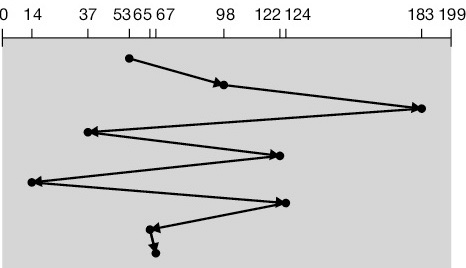
\includegraphics[width=0.25\linewidth]{images/scheduling_hdd_98.png}
\caption{Coda delle richieste: 98, 183, 37, 122, 14, 124, 65, 67 In tutto la testina attraversa 640 tracce. Invece che “122 - 14124” era meglio fare “122 - 124 - 14” }
\end{figure}

\subsubsection{C-SCAN (Circular-SCAN)}
Fornisce un tempo di attesa per le varie richieste più uniforme di altri algoritmi, anche se non riesce a garantire un tempo medio di attesa minimo.\\
La testina si muove da un estremo all’altro del piatto, servendo le richieste.\\
Quando raggiunge l’estremità del piatto, torna immediatamente all’inizio senza servire richieste.\\
In pratica, \textbf{tratta i settori/cilindri come una lista circolare.}\\

\begin{figure}[h] \centering \includegraphics[width=0.25\linewidth]{images/scheduling_hdd_cscan.png}
    \caption{Coda delle richieste: 98, 183, 37, 122, 14, 124, 65, 67 La testina attraversa 183 tracce + 200 tracce per tornare indietro, ma questo ritorno richiede poco tempo, perché la
    testina non deve mai fermarsi e ripartire}
\end{figure}

\nt{Questo è l'algoritmo di scheduling più utilizzato nei sistemi operativi moderni.}


\section{Formattazione del disco}
Prima di poter essere utilizzato, un disco rigido deve essere sottoposto a un processo di \textit{formattazione}, che avviene in due fasi principali:

\begin{itemize}
    \item Questa operazione viene solitamente effettuata dal costruttore dell’HD e ha lo scopo di:
    \begin{itemize}
        \item Associare un numero univoco a ogni settore.
        \item Allocare uno spazio per un codice di correzione degli errori (ECC), utilizzato durante ogni operazione di I/O su quel settore.
    \end{itemize}
    \item Durante questa fase è possibile definire la dimensione dei blocchi fisici, ad esempio 512 byte o 4096 byte per settore.
\end{itemize}

\subsubsection{Formattazione logica}

\begin{itemize}
    \item Questo processo, gestito dal sistema operativo, è necessario per creare e organizzare il File System.
    \item Il sistema operativo esegue le seguenti operazioni:
    \begin{itemize}
        \item Creazione della lista dei blocchi liberi secondo lo schema adottato.
        \item Creazione di una directory iniziale, punto di partenza per l’intera struttura del File System.
        \item Riservazione di aree specifiche per la gestione diretta da parte del SO:
        \begin{itemize}
            \item \textbf{Boot Block:} il blocco di avviamento.
            \item \textbf{Aree per gli attributi dei file:} ad esempio, gli \textit{index-node} in Unix o la MFT (\textit{Master File Table}) in Windows.
        \end{itemize}
    \end{itemize}
\end{itemize}

\subsection{Il Boot Block}

\begin{itemize}
    \item Contiene il codice necessario per avviare il sistema operativo.
    \item All’accensione, un piccolo programma residente in ROM istruisce il \textit{disk controller} a trasferire il contenuto del Boot Block nella RAM.
    \item Una volta trasferito, il controllo passa al codice del Boot Block, che avvia l’intero sistema operativo caricandolo dal disco stesso.
\end{itemize}

\section{Gestione dell'area di SWAP}
Durante la formattazione logica del disco rigido, il sistema operativo riserva uno spazio per l'\textit{area di Swap}, che funge da memoria virtuale utilizzata per lo scambio di pagine o segmenti tra RAM e memoria secondaria.

\subsection{Gestione dell'area di Swap}

\begin{itemize}
    \item \textbf{Swap come file:} 
    \begin{itemize}
        \item Nel caso più semplice, l’area di Swap può essere un file di grandi dimensioni all’interno del File System.
        \item Nei sistemi Windows, lo \textit{swap file} è denominato \texttt{pagefile.sys}. 
        \item Gli utenti possono regolarne la dimensione, ad esempio riducendola in presenza di una grande quantità di RAM, per recuperare spazio sul disco rigido.
    \end{itemize}

    \item \textbf{Swap come partizione dedicata:}
    \begin{itemize}
        \item Una porzione specifica del disco rigido, chiamata \textit{partizione di Swap}, può essere riservata esclusivamente a questo scopo.
        \item Questa partizione è gestita diversamente rispetto a un normale File System, adottando strategie di allocazione ottimizzate per la velocità di accesso.
        \item Ad esempio, i blocchi possono essere allocati in modo contiguo per evitare la ricerca di blocchi liberi, riducendo così il tempo necessario per lo scambio.
    \end{itemize}
\end{itemize}

\subsubsection{Dimensionamento dell'area di Swap}

\nt{
    È fondamentale dimensionare adeguatamente l’area di Swap per garantire che il sistema operativo trovi rapidamente uno spazio libero per lo scambio di pagine e segmenti.
}

\begin{itemize}
    \item \textbf{Consigli per il dimensionamento:}
    \begin{itemize}
        \item In Solaris, si raccomanda di dimensionare l’area di Swap in base alla differenza tra lo spazio di indirizzamento logico e quello fisico.
        \item In Linux, si suggerisce di utilizzare un’area di Swap pari al doppio della RAM disponibile.
    \end{itemize}
    
    \item \textbf{Sistemi con più dischi:}
    \begin{itemize}
        \item In configurazioni multi-disco, è possibile creare un’area di Swap per ciascun disco.
        \item Ciò consente di sfruttare le aree di Swap in parallelo, bilanciando il carico di lavoro e migliorando le prestazioni.
    \end{itemize}
\end{itemize}


\section{Sistemi RAID}
Gli hard disk (HD) e i dischi a stato solido (SSD) sono dispositivi notevolmente più lenti rispetto al processore e alla memoria primaria. Inoltre, il guasto di un disco rigido rappresenta un rischio significativo: in assenza di un back-up, i dati memorizzati possono essere irrimediabilmente persi o, nel migliore dei casi, non disponibili durante i tempi di riparazione.

\subsection{Introduzione ai sistemi RAID}

\dfn{RAID (Redundant Array of Independent Disks)}{
    È un sistema di configurazione della memoria secondaria progettato per migliorare sia le prestazioni sia l'affidabilità degli hard disk. 
}

\begin{itemize}
    \item RAID si rivela utile in ogni settore, ma è essenziale in contesti critici dove il servizio non può mai interrompersi, come nel settore finanziario e bancario.
    \item Il concetto di RAID fu introdotto nel 1988 da Patterson, Gibson e Katz, con l'acronimo iniziale \textit{Redundant Array of Inexpensive Disks}, successivamente ridefinito come \textit{Redundant Array of Independent Disks}.
    \item La controparte dei sistemi RAID è rappresentata da dispositivi SLED (\textit{Single Large Expensive Disk}).
\end{itemize}

\subsection{Caratteristiche principali di un sistema RAID}

\begin{itemize}
    \item Un sistema RAID è costituito da un insieme di dischi (detto \textit{disk array}) che viene visto dal sistema operativo come un singolo dispositivo di memorizzazione, più veloce e affidabile di un SLED.
    \item La gestione dei dischi è demandata al \textit{controller del RAID}, che si occupa di distribuire i dati secondo criteri specifici, senza necessità di modifiche al sistema operativo. 
    \item Questo vantaggio semplifica notevolmente la vita degli amministratori di sistema (\textit{system administrators}).
\end{itemize}

\subsection{Idee principali alla base di RAID}

Le due idee fondamentali di un sistema RAID sono:
\begin{enumerate}
    \item \textbf{Distribuzione dei dati:} L'informazione è suddivisa su più dischi per parallelizzare parte delle operazioni di accesso e migliorare le prestazioni.
    \item \textbf{Ridondanza dei dati:} L'informazione è duplicata su più dischi. In caso di guasto di un disco, il sistema può continuare a funzionare, recuperando i dati dal disco di backup.
\end{enumerate}

\subsection{Livelli di RAID}

Differenti schemi di implementazione delle idee sopra descritte hanno portato alla definizione di vari livelli RAID, numerati da 0 a 6. 
\nt{
    Da qui in poi, ci si discosta parzialmente dalla trattazione del libro di testo.
}
\subsection{RAID di Livello 0}

\nt{
    I sistemi RAID di livello 0, pur essendo inclusi nella famiglia RAID, non offrono ridondanza dei dati, quindi non aumentano l'affidabilità del sistema.
}

\dfn{RAID Livello 0}{
    Un'architettura RAID in cui il disco virtuale (cioè l'insieme di blocchi logici consecutivi visti dal sistema operativo) viene suddiviso in \textit{strip} (strisce) di $k$ blocchi consecutivi ciascuna. Questa tecnica, chiamata \textbf{striping}, distribuisce i dati su più dischi per migliorare le prestazioni.
}

\begin{itemize}
    \item Ogni \textit{strip} è identificata da un numero e contiene $k$ blocchi consecutivi.
    \begin{itemize}
        \item Lo strip 0 contiene i blocchi da $0$ a $k-1$.
        \item Lo strip 1 contiene i blocchi da $k$ a $2k-1$.
    \end{itemize}
    \item Gli strip sono distribuiti sui dischi disponibili secondo la formula:
    \[
    \text{numero-strip} \mod \text{dischi-nel-sistema}
    \]
    \item Ad esempio, in un sistema con 4 dischi:
    \begin{itemize}
        \item Il disco 0 conterrà gli strip 0, 4, 8, ...
        \item Il disco 1 conterrà gli strip 1, 5, 9, ...
    \end{itemize}
    \item Se $k=1$, ogni strip contiene un singolo blocco. In questo caso:
    \begin{itemize}
        \item Il blocco 0 sarà sul primo settore del primo disco.
        \item Il blocco 1 sarà sul primo settore del secondo disco.
        \item Il blocco 4 sarà sul secondo settore del primo disco, e così via.
    \end{itemize}
\end{itemize}

\ex{Esempio di richiesta su un RAID Livello 0}{
    Supponiamo che il sistema operativo richieda la lettura di dati contenuti negli strip 4, 5, 6 e 7. 
    \begin{itemize}
        \item Il controller RAID suddividerà la richiesta in quattro letture parallele, una per ciascun disco.
        \item Su un singolo disco SLED, invece, tutti i settori dei quattro strip dovrebbero essere letti in sequenza.
    \end{itemize}
    Di conseguenza, l'operazione sarà completata più rapidamente con il RAID 0.
}

\clm{Prestazioni e limiti del RAID Livello 0}{}{
    \begin{itemize}
        \item \textbf{Miglioramenti delle prestazioni:} Un RAID di livello 0 è particolarmente efficiente quando le richieste coinvolgono molti strip consecutivi, e il sistema è composto da un elevato numero di dischi.
        \item \textbf{Limitazioni:}
        \begin{itemize}
            \item Richieste che riguardano un singolo strip non ottengono alcun miglioramento rispetto a un disco SLED.
            \item L'affidabilità del sistema è inferiore a quella di un singolo disco SLED, poiché il \textit{Mean Time To Failure} (MTTF) complessivo diminuisce con l'aumento del numero di dischi.
        \end{itemize}
        \item \textbf{Applicazioni tipiche:} Il RAID 0 è utilizzato in applicazioni che richiedono alte prestazioni ma non necessitano di particolare affidabilità, come lo streaming audio e video.
    \end{itemize}
}
\begin{figure}[h] \centering \includegraphics[width=0.50\linewidth]{images/raid_livelloZero.png} \caption{Raid Livello Zero} \label{fig:2-23a} \end{figure}


% %---------------------------------------


\afterpage{\blankpage}
\setcounter{chapter}{98}
\chapter{Esercizi}
\section{Capitolo 5}
\subsection{1}
% Requires: \usepackage{amsmath}
\begin{table}[h]
    \centering
    \begin{tabular}{c c c}
        \underline{Processo} & Durata & priorità \\
        $P_1$ & 10 & 3 \\
        $P_2$ & 1 & 1 \\
        $P_3$ & 2 & 3 \\
        $P_4$ & 1 & 4 \\
        $P_5$ & 5 & 2 \\
    \end{tabular}
    \caption{Processi con durata e priorità}
    \label{tab:processi}
\end{table}
\textbf{FCFS}:
\[
\begin{array}{|c|c|c|c|c|}
  \hline
  \mathbf{P_1} & \mathbf{P_2} & \mathbf{P_3} & \mathbf{P_4} & \mathbf{P_5} \\
  \hline
\end{array}
\]
\textbf{SJF}:
\[\begin{array}{|c|c|c|c|c|}
  \hline
  \mathbf{P_2} & \mathbf{P_4} & \mathbf{P_3} & \mathbf{P_5} & \mathbf{P_1} \\
  \hline
\end{array}\]


\end{document}